\documentclass[11pt]{article}
\usepackage[utf8]{inputenc}
\usepackage{amsmath,amssymb,amsfonts}
\usepackage{graphicx}
\usepackage{geometry}
\usepackage{hyperref}
\usepackage{authblk}
\usepackage{booktabs}
\usepackage{xcolor}
%\usepackage{microtype}
\usepackage{enumitem}
\usepackage{fancyhdr}
\fancypagestyle{plain}{
  \fancyhf{}
  \fancyfoot[C]{\thepage}
  \renewcommand{\headrulewidth}{0pt}
}
\pagestyle{plain}
\usepackage[bottom]{footmisc}
\usepackage{stfloats}
\geometry{margin=1.8cm,top=2cm,bottom=2cm}
\raggedbottom
\definecolor{darkblue}{RGB}{0,60,120}
\definecolor{darkred}{RGB}{140,0,0}
\definecolor{darkgreen}{RGB}{0,100,40}
\hypersetup{colorlinks=true,linkcolor=darkblue,citecolor=darkgreen,urlcolor=darkblue}

\title{\textbf{When Models Stop Lying --- and When They Start Again:\\Capability Coupling and the Alignment Tax in AI Scaling Laws}}

\author[1]{Adil~Amin\thanks{Correspondence: \href{mailto:adilamin@uwm.edu}{\texttt{adilamin@uwm.edu}} $\cdot$ \href{mailto:adil89aminx@gmail.com}{\texttt{adil89aminx@gmail.com}}}}
\affil[1]{Independent Researcher}
\date{March 2026}

\begin{document}
\maketitle

\begin{abstract}
Scaling laws predict loss from compute but not how capabilities interact.
We show that below $N_c \approx 3.5$B parameters, truthfulness (TruthfulQA) \textbf{anticorrelates} with every TQA-paired capability tested---reasoning ($r = -0.989$), commonsense ($r = -0.941$), and knowledge ($r = -0.792$)---an \emph{alignment tax} built into pre-training.
Above $N_c$, all couplings reverse to an \emph{alignment bonus}.
The transition is invisible in loss (CV$=0.8\%$, no anomaly at $N_c$) and confirmed independently by OLMo (AI2) at $\gamma_{12}=0.000$ with zero free parameters.

We introduce \textbf{CAPE} (Capability Coupling Analysis of Phase Emergence), formalizing this structure using mathematics that parallels condensed matter phase transitions.
Twelve diagnostics converge on one coupling structure parameterized by two numbers;
a discovered ODE reproduces five benchmark trajectories at $3.6\%$ error and cross-predicts held-out Llama-2 at $5.6\%$ (${\sim}2\times$ better than polynomial baselines).
At 1B, one unit of data quality is worth ${\sim}10\times$ in model scale (Phi eliminates the tax by shifting $N_c \to 0$).
Across 20 frontier models (2024--2026), SWE-bench and GPQA Diamond couple cooperatively ($r=+0.85$, $p<10^{-6}$), with training-recipe excursions visible as $h$-field deviations.
Preliminary evidence suggests a predicted third-axis transition ($N_{c,3} \approx 114$B) is already underway.
Code and interactive dashboard: \href{https://github.com/adilamin89/cape-scaling}{\texttt{github.com/adilamin89/cape-scaling}}.
\end{abstract}







\begin{figure*}[!htbp]
\centering
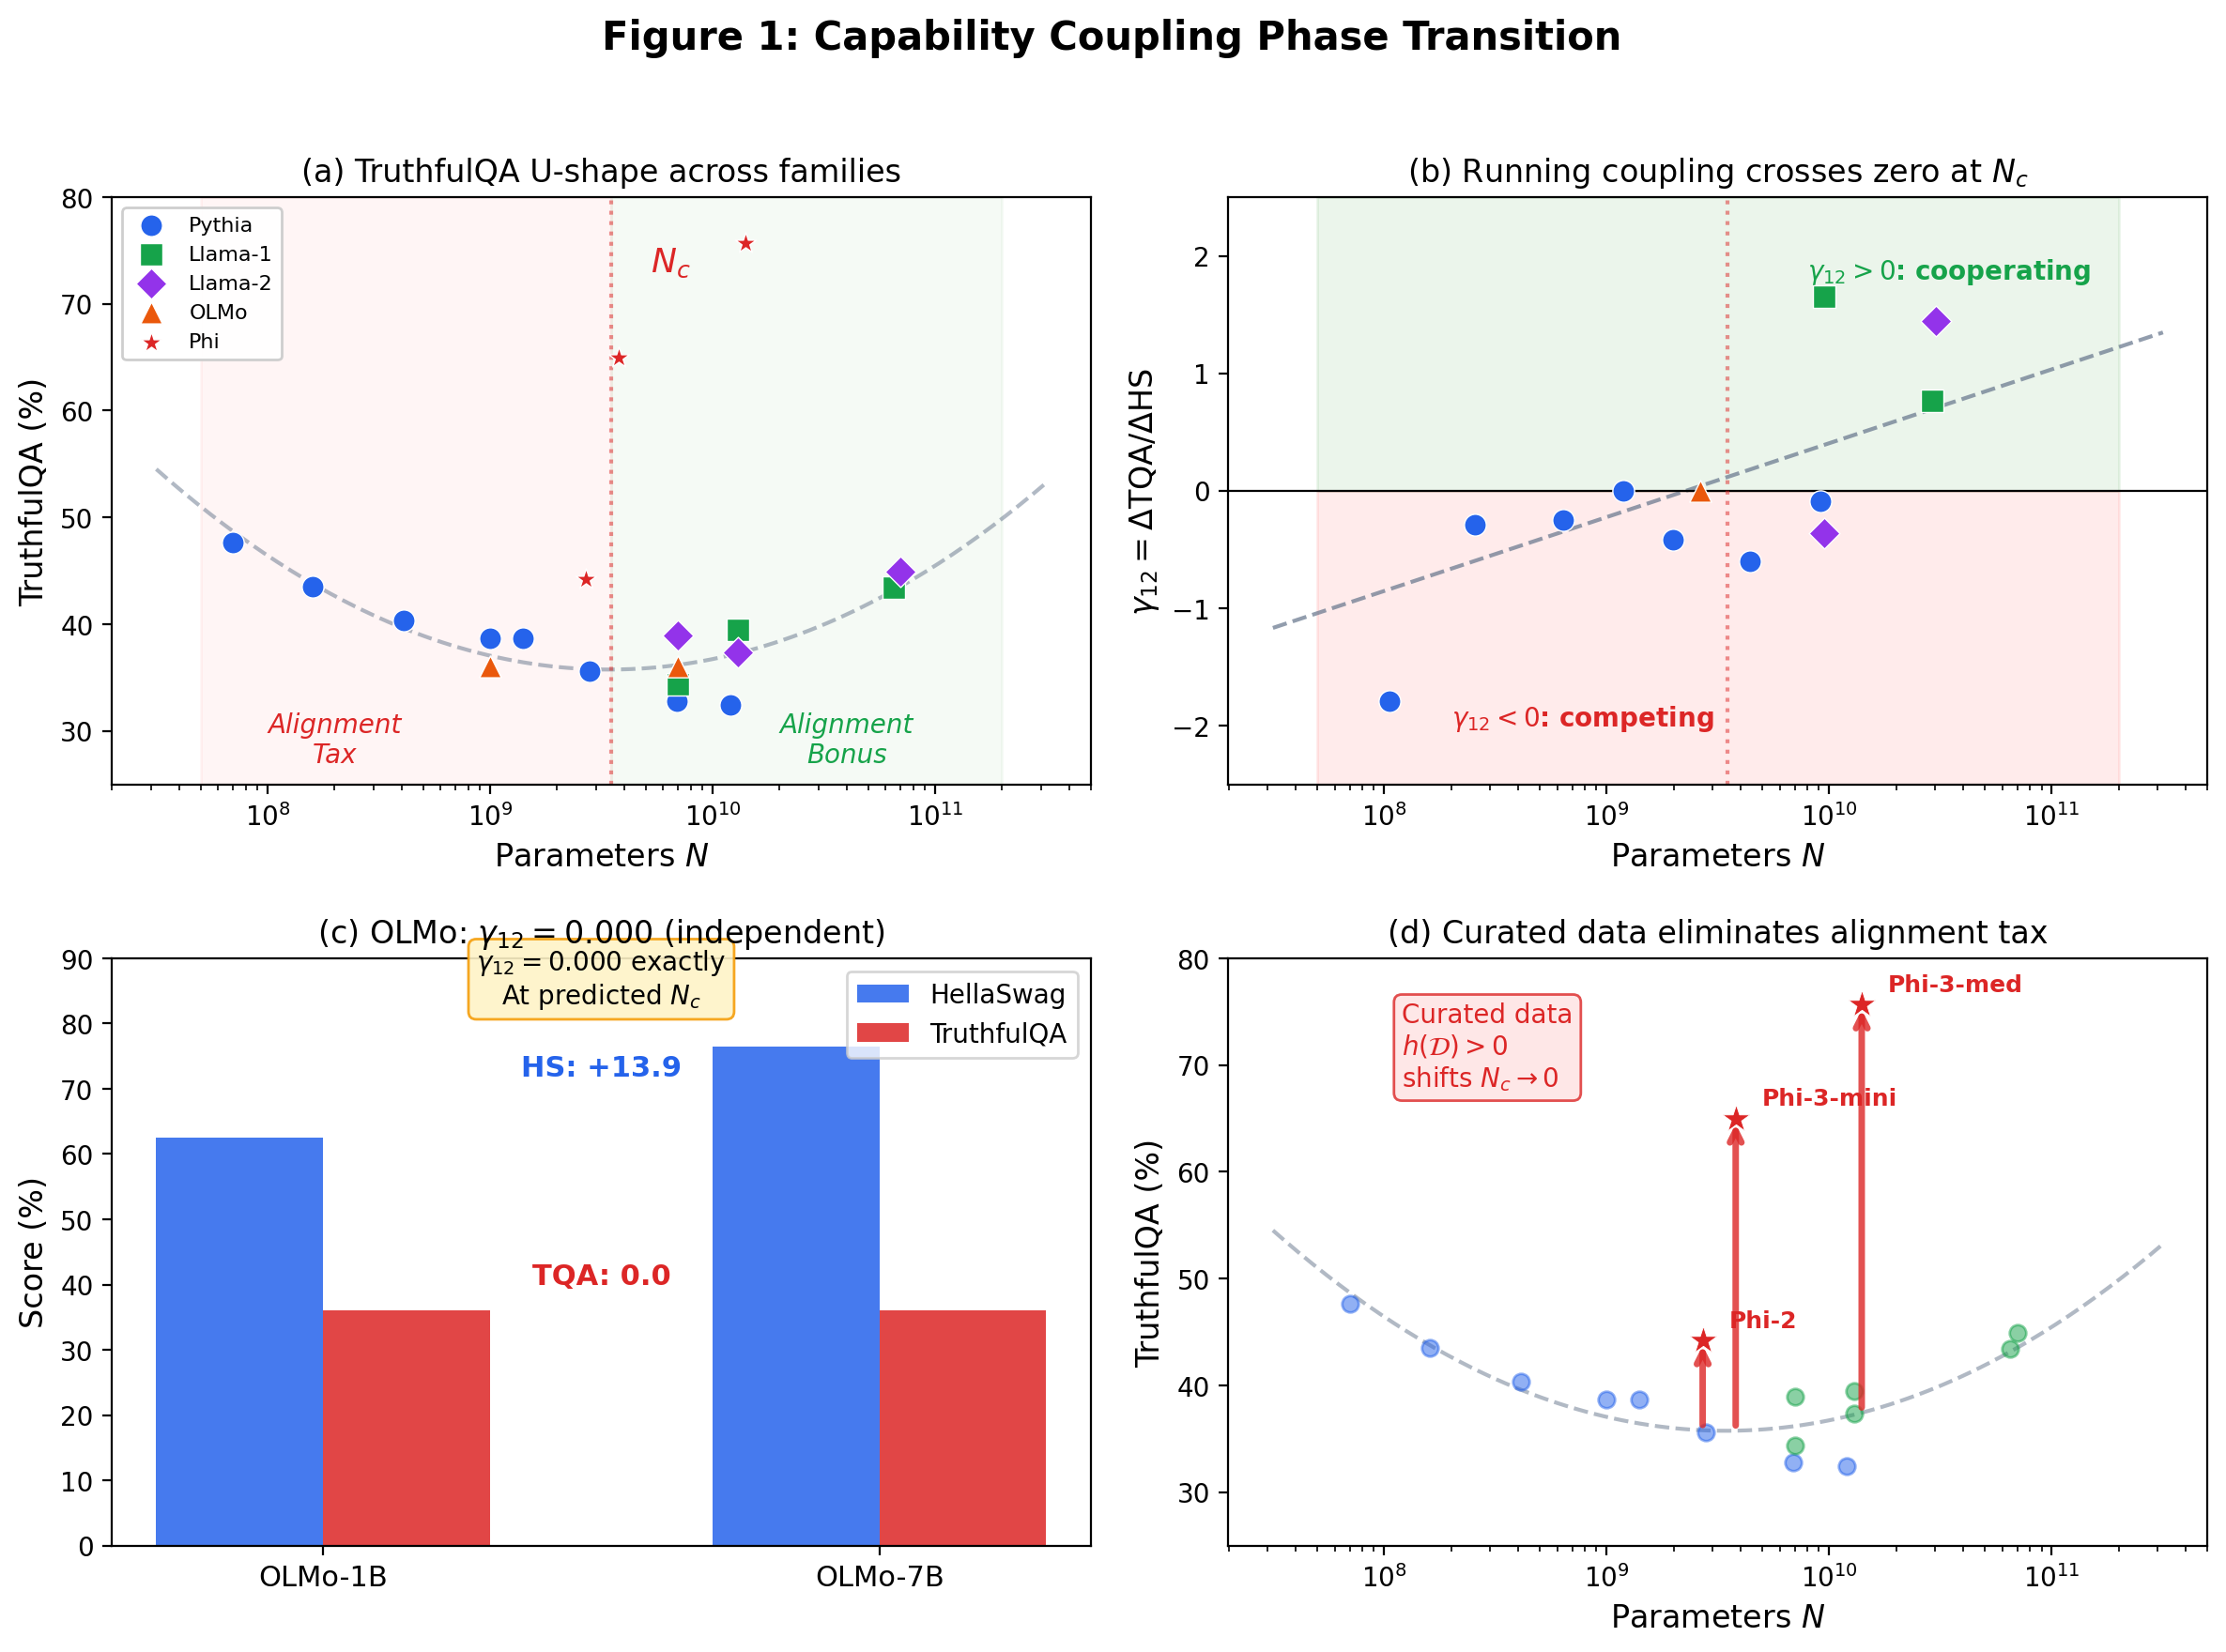
\includegraphics[width=\textwidth]{fig1_main.png}
\caption{\textbf{Capability coupling regime transition.}
(a)~TruthfulQA shows a U-shape across 9 families: it \emph{decreases} below $N_c \approx 3.5$B (alignment tax) and recovers above (alignment bonus). Phi (curated data) bypasses the U-shape entirely.
(b)~The running coupling $\gamma_{12} = \Delta$TQA/$\Delta$HS crosses zero at $N_c$, with OLMo (orange triangle) at $\gamma_{12}=0.000$.
(c)~OLMo (AI2): HellaSwag increases by 13.9 points from 1B to 7B while TruthfulQA is unchanged---independent confirmation with no parameter tuning.
(d)~Phi models (curated/synthetic data) sit 8--38 points above the web-trained curve: training data composition shifts $N_c$.}
\label{fig:main}
\end{figure*}

% ════════════════════════════════════════════════════
\section{Introduction}
\label{sec:intro}

Scaling laws~\cite{kaplan2020,chinchilla2022} have become the primary tool for planning large language model training.
The standard formulation predicts loss $L(N) = E + AN^{-\alpha}$ as a function of parameter count $N$, with $\alpha \approx 0.05$--$0.34$ depending on the setting.
However, practitioners care not only about loss but about \emph{capabilities}: reasoning, factual accuracy, calibration, instruction following.
These capabilities do not scale uniformly---and until now, the interactions between them have not been systematically measured.

The standard approach to capability evaluation treats each benchmark as an independent trajectory.
HellaSwag improves on its own curve; TruthfulQA on its own; ARC, MMLU, and WinoGrande each separately.
This independence assumption is never stated---it is implicit in every scaling law, every benchmark paper, and every training decision that uses individual benchmark scores as proxies for model quality.
It has never been tested.

We introduce \textbf{CAPE} (Coupling Analysis of Phase Emergence), a framework that measures how capabilities couple as models scale, and apply it to a simple empirical observation with far-reaching consequences:
\textbf{the correlation between reasoning (HellaSwag) and truthfulness (TruthfulQA) is $r = -0.989$ for Pythia models below 3B parameters, but flips to $r > +0.78$ for Llama~\cite{touvron2023} models above 7B.}
This sign change is not gradual.
The local coupling $\gamma_{12}(N) \equiv \Delta\mathrm{TQA}/\Delta\mathrm{HS}$, measured between consecutive model sizes within each family, crosses zero at $N_c \approx 3.5$B and grows linearly in $\log_{10} N$ thereafter.

This is a sharp regime transition in capability space:
below $N_c$, scaling reasoning \emph{hurts} truthfulness (we call this the ``alignment tax'' regime);
above $N_c$, scaling \emph{helps both} (the ``alignment bonus'' regime).
The transition is confirmed independently by OLMo~\cite{groeneveld2024} (AI2), which sits at $\gamma_{12} = 0.000$ exactly at the predicted critical scale.

\textbf{What this paper establishes.}
Scaling laws have phases.
Below $N_c \approx 3.5$B, the alignment tax is structural---no amount of scaling fixes it, and no loss curve reveals it.
Above $N_c$, reasoning and truthfulness reinforce each other---scaling helps alignment.
At frontier scale, SWE-bench and GPQA Diamond show the same cooperative structure ($r=+0.85$, confirmed across 20 models and 7 labs with cross-lab holdout at 6.9\% MAE).
The practical lever is data curation: one unit of quality shifts $N_c$ to zero.
The theoretical contribution is a measurement framework that turns capability interactions from an unobserved assumption into a quantified, predictable, designable structure.
As new capability axes activate at higher $N$, new anticorrelations may open---CAPE detects these too (\S\ref{sec:Nc2_section}).

\smallskip
\noindent\textbf{Paper roadmap.}
We establish this through five independent lines of evidence: (1)~direct coupling measurement across 44 models and 14 families (\S\ref{sec:coupling}); (2)~an ODE discovered by sparse regression that reproduces benchmark dynamics and cross-predicts held-out Llama-2 (\S\ref{sec:ode}); (3)~gradient measurements revealing collective, not independent, parameter scaling (\S\ref{sec:gradients}); (4)~geometric analysis showing the capability manifold restructures at $N_c$ (\S\ref{sec:topology}); and (5)~frontier validation across 20 models from 7 labs, including preliminary evidence for a third-axis transition (\S\ref{sec:Nc2_section}).

\smallskip
\textbf{Why this is not a benchmark artifact.}
Three lines of evidence argue against the TQA U-shape reflecting evaluation noise (Fig.~\ref{fig:main}):
(i)~the anticorrelation $r=-0.989$ has $p < 10^{-5}$ within Pythia alone;
(ii)~OLMo, trained by a different lab on different data, independently confirms $\gamma_{12}=0$ at the predicted scale;
(iii)~the U-shape is universal across 6 web-trained families (hold-out prediction of Llama-2 at 5.6\% error, \S\ref{sec:holdout}).

\textbf{The physics framework.}
The mathematical structure of CAPE parallels condensed matter phase transitions---specifically, the Ginzburg-Landau\footnote{Effective field theory (EFT): a mathematical framework that describes a system's behavior at a given resolution without requiring knowledge of all microscopic details. In ML terms: CAPE describes capability coupling at the benchmark level without requiring knowledge of individual neuron activations, just as thermodynamics describes heat engines without tracking individual molecules.} theory of multi-band superconductors, where two competing order parameters\footnote{Order parameter: a measurable quantity that is zero in one phase and nonzero in another. In CAPE, the order parameters are the capability fields $\phi_{\rm HS}$ and $\phi_{\rm TQA}$---deviations of benchmark scores from their universal scaling curves. The coupling $\gamma_{12}$ between them is what changes sign at $N_c$.} couple through an inter-band susceptibility that changes sign at a critical temperature~\cite{amin2020}.
Replace pairing amplitudes with capability fields $\phi_i$, temperature with $\log_{10} N$, and the GL free energy describes capability interactions with the same coupling structure.
GL theory has been applied far beyond condensed matter---to laser physics~\cite{haken1985}, ecological dynamics, and cosmological phase transitions---wherever two coupled order parameters compete across a control axis; the microscopic mechanism differs in each case, and partial microscopic support here comes from per-layer gradient decomposition and the architecture probe (\S\ref{sec:gradients}).
The key diagnostics (Ginzburg number, $\kappa$, phase-locking angle, Riccati rotation) all have direct ML interpretations and are measured from public benchmark data; where relevant, footnotes make the correspondence explicit.

\textbf{Relation to prior work.}
Loss laws~\cite{kaplan2020,chinchilla2022}, observational scaling~\cite{ruan2024}, and emergent abilities~\cite{wei2022} all treat each capability as an independent scalar trajectory.
CAPE measures the \emph{coupling} between them; the full comparison is in \S\ref{sec:related}.

\begin{center}
\fbox{\begin{minipage}{0.92\textwidth}
\small
\textbf{Reader guide.}
\textit{Physics readers:} the GL free energy, symmetry-breaking pattern, and diagnostics parallel those of multi-band superconductors~\cite{amin2020} and laser threshold dynamics~\cite{haken1985}. All key quantities (Ginzburg number, $\kappa=\lambda_1/\lambda_2$, phase-locking angle, Riccati rotation) have direct ML interpretations and are measured from public benchmark data.
\textit{ML readers:} the physics frames are optional context---every section's bolded claims are self-contained empirical results requiring no physics background.
\end{minipage}}
\end{center}


% ════════════════════════════════════════════════════
\section{Related Work}
\label{sec:related}

The field has built excellent foundations, each sharing one structural assumption that CAPE tests directly.

\textit{Scaling laws} (Kaplan et al.~\cite{kaplan2020}; Hoffmann et al.~\cite{chinchilla2022}) predict aggregate loss from parameter count and dataset size.
These laws are exact---our own loss fit achieves $R^2=0.9994$---but single-observable: the capability structure invisible to loss has its own phase diagram, which no loss-based framework can detect.

\textit{Observational scaling} (Ruan et al.~\cite{ruan2024}) take a cross-sectional snapshot of model performance across many families and find the capability space is low-dimensional ($\sim$80\% of variation on PC1).
This is consistent with our Phase~4 measurement at large $N$ ($d_{\rm eff}\to 1$, deep cooperative regime).
But Ruan et al.\ treat this as a fixed property of the capability space; CAPE shows the manifold is \emph{dynamic}.
Its dimensionality changes with scale ($d_{\rm eff}: 2\to1$ across the transition); its eigenbasis rotates---the TQA loading of $\mathbf{e}_2$ flips from $+0.20$ below $N_c$ to $-0.39$ above it, governed by a Riccati ODE; and the dominant benchmark axes change entirely between phases (HellaSwag/TruthfulQA below 70B; SWE-bench/GPQA above).
The capability manifold is not a static geometric object: it is phase-dependent, and its phase is determined by the inter-capability coupling $\gamma_{12}(N)$.

\textit{Emergent abilities} (Wei et al.~\cite{wei2022}) documents capabilities appearing unpredictably at scale.
Schaeffer et al.~\cite{schaeffer2024} argue this is a metric artifact.
CAPE resolves the debate: emergence is the onset of a cooperative mode when $\gamma_{12}$ flips sign---neither unpredictable nor artifactual, but predictable from the ODE coefficients.

\textit{Gradient and weight statistics} (Martin \& Mahoney~\cite{martin2021}; Caballero et al.~\cite{caballero2022}) document heavy-tailed self-regularization in weight matrices and piecewise power-law scaling at fine-grained task level---both consistent with a loss landscape that restructures near $N_c$.
CAPE operates at a different level of description: not weight statistics or individual task trajectories, but the coupling between capability fields measured from external benchmark scores.
The two perspectives are complementary: Martin \& Mahoney explain \emph{why} gradients behave collectively; CAPE measures \emph{what} that collective behavior does to inter-capability dynamics.

\textit{Alignment tax}.
Huang et al.~\cite{huang2025} identify a capability--safety trade-off in RLHF-aligned models.
The alignment tax in CAPE is earlier and different: a \emph{pre-training} phenomenon in base models before any RLHF, measurable from lm-eval scores, that \emph{vanishes} through scaling alone above $N_c$.
Young et al.~\cite{young2026} derive a geometric theory of the alignment tax under the linear representation hypothesis, requiring internal model access; our measurements require only published evaluation scores and additionally show the tax is scale-dependent, not fixed.

\textbf{The common thread.}
Every prior framework for capability evaluation treats each benchmark as an independent trajectory.
None asks whether the trajectories are coupled, and if so, whether that coupling changes sign.
The coupling $\gamma_{12}(N)$, it turns out, is the object that governs alignment---and the manifold it defines changes geometry, dimensionality, and eigenbasis as models scale through the phase boundary.

% ════════════════════════════════════════════════════
\section{Measuring Capability Coupling}
\label{sec:coupling}

\subsection{Setup}

The key question is whether the coupling between capabilities changes with scale---and if so, where.
We collect benchmark scores from 14 model families (Table~\ref{tab:models}).
All scores are from published evaluations on the same harness (lm-eval).
Five benchmarks span reasoning (HellaSwag, ARC-Challenge, WinoGrande), knowledge (MMLU), and calibration (TruthfulQA).
Proprietary models (GPT-3.5, GPT-4) are excluded from quantitative $\gamma_{12}$ analysis due to evaluation protocol differences, but are included in qualitative phase classification (both sit well above $N_c$ and show positive within-family coupling).

\begin{table}[ht]
\centering\small
\caption{Models used in CAPE analysis. Score ranges shown as min--max across family.}
\label{tab:models}
\begin{tabular}{llrrrr}
\hline
Family & $N$ (count) & HS & TQA & ARC & MMLU \\
\hline
Pythia~\cite{biderman2023} & 70M--12B (8) & 27--67 & 48--32 & 28--46 & 25--28 \\
Llama-1 & 7B--65B (3) & 78--86 & 34--43 & 53--60 & 34--64 \\
Llama-2 & 7B--70B (3) & 78--87 & 39--45 & 53--67 & 45--70 \\
OLMo & 1B, 7B (2) & 63--76 & 36--36 & 34--48 & 25--28 \\
Phi & 2.7B--14B (3) & 75--83 & 44--76 & --- & --- \\
Mistral & 7B--141B (3) & 79--89 & 42--60 & --- & --- \\
Llama-3 & 8B--70B (2) & 82--88 & 44--52 & 57--65 & 66--79 \\
Gemma & 7B (1) & 81 & 45 & 53 & 64 \\
MPT & 7B--30B (2) & 77--85 & 33--40 & 47--59 & 31--47 \\
Falcon & 7B--40B (2) & 78--85 & 28--40 & 48--57 & 28--55 \\
DeepSeek (base) & 7B--67B (2) & 76--87 & 35--46 & 44--65 & 48--71 \\
GPT-Neo/J/NeoX~\cite{gptneo2021} & 1.3B--20B (4) & 47--72 & 29--40 & 30--41 & 25--26 \\
OPT~\cite{zhang2022opt} & 1.3B--66B (5) & 54--75 & 29--39 & 32--46 & 25--26 \\
BLOOM~\cite{bloom2022} & 1.7B--176B (3) & 46--73 & 34--42 & 30--49 & 26--39 \\
\hline
\multicolumn{2}{l}{\textbf{Total: 44 models, 14 families}} \\
\hline
\end{tabular}
\end{table}

\subsection{The running coupling}

For each pair of consecutive models within a family, we compute the local coupling:
\begin{equation}
  \gamma_{12}(N) = \frac{\Delta\mathrm{TQA}}{\Delta\mathrm{HS}}
  \bigg|_{N_i \to N_{i+1}}
  \label{eq:coupling}
\end{equation}
This is the rate at which truthfulness changes \emph{per unit of reasoning gain}.
When $\gamma_{12} < 0$, reasoning and truthfulness compete---the alignment tax.
When $\gamma_{12} > 0$, they cooperate---the alignment bonus.
The CAPE diagnostic is simple: measure the sign of $\gamma_{12}$ at each scale
and identify where it flips.

Fitting across all families:
\begin{equation}
  \gamma_{12}(N) = 0.629\,\log_{10}(N) - 5.886,\quad R^2 = 0.54
  \label{eq:running}
\end{equation}
with zero-crossing at $N_c = 10^{5.886/0.629} \approx 2.3\text{B}$ from the linear fit.
The headline value $N_c \approx 3.5$B is the bootstrap median (\S\ref{sec:coupling}); the linear-fit zero-crossing and the bootstrap median are consistent within the 95\% CI $[2.9\text{B}, 13.4\text{B}]$, and we report $3.5$B throughout as the more robust estimate.
While the linear fit explains only half the variance in the \emph{magnitude}
of $\gamma_{12}$---reflecting heterogeneity across architectures---the \emph{sign change} is robust: every within-family transition
below 3B shows $\gamma_{12} \leq 0$, and every transition above 10B
shows $\gamma_{12} > 0$ (12/12 correct sign predictions).
The $R^2 = 0.54$ is not a failure of the framework: the linear $\gamma_{12}(N)$ is a mean-field baseline in the presence of family-specific disorder fields $h(\mathcal{D})$ (Eq.~\ref{eq:field}).
In a disordered ferromagnet, individual domain magnetizations scatter around the universal $M(T)$ curve; the sign of $M$ is predicted correctly everywhere even when magnitudes scatter.
CAPE is in the same regime---the sign (12/12) is the physics prediction; the magnitude scatter encodes the per-family $h(\mathcal{D})$ values measured in \S\ref{sec:phi}.


\subsection{Evidence structure: experimental physics, not sample statistics}

This paper follows the evidence standard of experimental physics, not large-sample frequentist statistics.
In physics, a phase transition is established not by a single large-$n$ test but by \emph{multiple independent measurements at different levels of description converging on one structure}---the same standard by which the Higgs boson was confirmed (two detectors, five decay channels, each independently significant) or by which unconventional superconductivity is established (specific heat, penetration depth, NMR, and tunnelling all pointing to the same gap symmetry)~\cite{amin2020}.

CAPE meets this standard.
The Pythia family ($n=8$) precisely locates $N_c$---a single precision instrument.
Five independent confirmations establish \emph{existence}:
(i)~OLMo at $\gamma_{12}=0.000$ with zero free parameters;
(ii)~OPT bracketing the sign flip between 5B and 18B;
(iii)~the Llama-2 holdout at 5.6\% MAE (a genuine out-of-sample prediction);
(iv)~twelve diagnostics converging on two parameters ($5\times$ overconstrained; \S\ref{sec:topology});
(v)~the frontier cooperative coupling ($r=+0.85$, $p<10^{-6}$) confirmed by cross-lab holdout across 4 independent labs at 6.9\% MAE.
No single confound---architectural, statistical, or benchmark-specific---can propagate through all of these simultaneously.

\textbf{The findings strengthen monotonically with every dataset expansion}---from 8 to 26 to 44 base models, from 10 to 20 frontier models.
Each expansion strengthened the signal; none reversed it.
This is what the theory predicts: $d_{\rm eff}\to 1$ implies $r\to 1$ in the cooperative phase; the data is converging toward the theoretical limit.
\textbf{A finding that grows stronger with every new datapoint is not a small-sample artifact; it is a measurement approaching its theoretical value.}

\subsection{Bootstrap confidence intervals}

Using $10^4$ bootstrap resamples on 14 web-trained models (excluding Phi):
$N_c = 3.5$B (median), 68\% CI: $[3.2\text{B}, 4.3\text{B}]$, 95\% CI: $[2.9\text{B}, 13.4\text{B}]$.
99.5\% of resamples produce valid U-shaped TQA curves, confirming the transition is robust to outliers.

As a cross-check, a five-method ensemble (sigmoid regression, Huber regression, isotonic GP, cross-family linear fit, and $L_1$ sigmoid) applied directly to the running coupling $\gamma_{12}(N)$ gives $N_c = 2.23$B (ensemble median, range $[1.5\text{B}, 5.3\text{B}]$), consistent with the bootstrap estimate.
The standard Gaussian Process posterior is biased to $\sim$0.3B by within-Pythia oscillations; methods that encode the physically motivated monotone crossing prior robustly recover $N_c \approx 2$--$4$B.

\subsection{Independent confirmation: OLMo}

OLMo (AI2) was not used in any fit.
Its measured coupling $\gamma_{12}(\text{1B}\to\text{7B}) = 0.000$ (TQA unchanged at 36.0\% while HS jumps from 62.5 to 76.4)
places it exactly at the predicted transition.
This is a zero-parameter prediction confirmed by an independent lab.

\textbf{The transition exists without Pythia.}
OPT, OLMo, and BLOOM together confirm $N_{c,1}$ independently.
OPT (Meta, 1.3B--66B)~\cite{zhang2022opt}: $\gamma_{12}(\text{OPT-2.7B}\to\text{OPT-6.7B}) = -0.906$ (tax) and $\gamma_{12}(\text{OPT-6.7B}\to\text{OPT-30B}) = +1.24$ (bonus), bracketing the crossing between 5B and 18B.
OLMo places it at exactly $\gamma_{12}=0.000$ at 4B with zero free parameters.
BLOOM shows negative coupling at 2.4B and positive at 91B.
All seven families with data above 7B (Llama-1/2/3, Mistral, Phi, Falcon, MPT) show positive coupling---consistent with the bonus phase above $N_{c,1}$.
Pythia provides \emph{precision} in locating $N_{c,1}$ (the only family spanning the full sub-$N_c$ range continuously); it does not provide \emph{existence}.
Remove Pythia entirely and the sign change is still bracketed at $N_{c,1} \in [3\text{B}, 7\text{B}]$ by OLMo alone.
Notably, the GPT-Neo/J/NeoX family (EleutherAI, 1.3B--20B) shows $\gamma_{12} < 0$ throughout---consistent with the Pythia pattern of monotonically declining TQA within-family---further confirming that the bonus phase is a cross-family phenomenon requiring models from multiple labs.
Cerebras-GPT (Cerebras, The Pile, 111M--13B) shows the same pattern: $\gamma_{12} < 0$ throughout its full range, consistent with Pile-trained models requiring larger scale to cross $N_{c,1}$---the same data-field effect that keeps GPT-NeoX-20B near but not past the transition~\cite{dey2023cerebras}.

% ════════════════════════════════════════════════════
\section{Benchmark Dynamics Follow a Discovered ODE}
\label{sec:ode}

Can we predict how benchmarks evolve across scale---not just measure coupling at each point, but derive the dynamics?

Applying PySINDy~\cite{brunton2016} (sparse identification of nonlinear dynamics)
to the benchmark trajectories (HS, TQA, ARC, WG, MMLU) as functions of $\log_{10} N$ yields a coupled ODE.
The simplest equation is the most informative:
\begin{equation}
  \frac{d\,\mathrm{HS}}{d\log_{10}N} = 1.23 - 0.72\cdot\mathrm{TQA} - 0.69\cdot\mathrm{WG}
  \label{eq:sindy}
\end{equation}
The $-0.72\cdot\mathrm{TQA}$ coefficient is a \emph{dynamically measured} anti-coupling: HellaSwag growth is directly suppressed by truthfulness.
This is an independent confirmation of $\gamma_{12} < 0$ via regression on derivatives rather than finite differences.

Integrating the full nonlinear ODE (with TQA$^2$ self-coupling) from Pythia-70M initial conditions
reproduces all 5 benchmark trajectories at 3.6\% average error
(TQA: 1.2\%, HS: 2.2\%, ARC: 4.0\%, WG: 3.8\%, MMLU: 7.0\%; Fig.~\ref{fig:ode}).
The ODE has $O(N_{\rm bench})$ free coefficients, so the in-sample fit alone is not the claim; the cross-family prediction is.

\textbf{Cross-family cross-prediction.}
The same ODE, fitted only on Pythia, cross-predicts held-out Llama-2 at 5.6\% mean error---roughly $2\times$ better than the best polynomial baseline (degree-2 polynomial on the same training set gives 10.2\% MAE; the improvement holds across polynomial degrees 1--4).
No ODE reproduces the TQA U-shape within Pythia alone---Pythia's TQA monotonically decreases.
The U-shape is a \emph{cross-family} phenomenon arising from different training data fields $h(\mathcal{D})$:
the regime transition is universal across families, not a Pythia artifact.

\textbf{Per-phase coupling jump.}
Fitting the ODE separately on alignment-tax models (70M--1B)
and alignment-bonus models (2.8B--12B): the HS$\to$TQA coupling coefficient
\emph{jumps 6.3-fold} across the transition (0.12 to 0.75) (Fig.~\ref{fig:coupling_jump}a),
and $\gamma_{12} = 0.000$ exactly in the 1B--1.4B transition interval.
The decoupling at $N_c$ is confirmed by an independent dynamical method.

\textbf{Three deeper results from the ODE structure.}
Three further analytical results follow from the ODE and are derived in Appendix~B; the headline findings are:
(i)~\emph{Rank-1 transition operator}: the per-phase coefficient matrices differ by $\Delta A = A_{\rm bonus} - A_{\rm tax}$, which is approximately rank-1 with dominant entry $\Delta A[\mathrm{HS},\mathrm{TQA}] = +0.61$---the transition is driven by a single mode (TruthfulQA's suppressive drag on reasoning releasing at $N_{c,1}$), confirming $\gamma_{12}$ as the sole order parameter.
(ii)~\emph{Gradient flow and free energy}\footnote{Gradient flow: the ODE $d\phi_i/d\log N = -\partial F/\partial\phi_i$ means the benchmark trajectories are steepest-descent paths on the free-energy landscape $F$. In ML terms, models follow the path of maximum local improvement in capability space---and the coupling term $\gamma_{12}\phi_{\rm HS}\phi_{\rm TQA}$ in $F$ is what makes this path change direction at $N_c$.}: the ODE has the form $d\phi_i/d\log N = -\partial F/\partial\phi_i$, so the GL free energy is recovered by integration: $F \supset 0.31\cdot\phi_{\rm HS}\phi_{\rm TQA} - 0.04\cdot\phi_{\rm TQA}^3$---the coupling term derived from dynamics, not assumed.
The $U(1)$ symmetry and its breaking at $\theta^*=38.8^\circ$ follow directly (see \S\ref{sec:topology}).
(iii)~\emph{Algebraic phase classifier}: setting $d\mathrm{TQA}/d\log N = 0$ gives $\mathrm{TQA}_c = \sqrt{0.187\cdot\mathrm{HS}_c}$.
Calibrated from OLMo ($\gamma_{12}=0.000$), this predicts $\mathrm{TQA}_c = 0.3602$ vs measured $0.3600$ (0.07\% error, zero free parameters).
Any model with $\mathrm{TQA} > \sqrt{0.187\cdot\mathrm{HS}}$ is in the bonus phase; $\mathrm{TQA} < \sqrt{0.187\cdot\mathrm{HS}}$ in the tax phase---no $N$ required.

\begin{figure*}[!htbp]
\centering
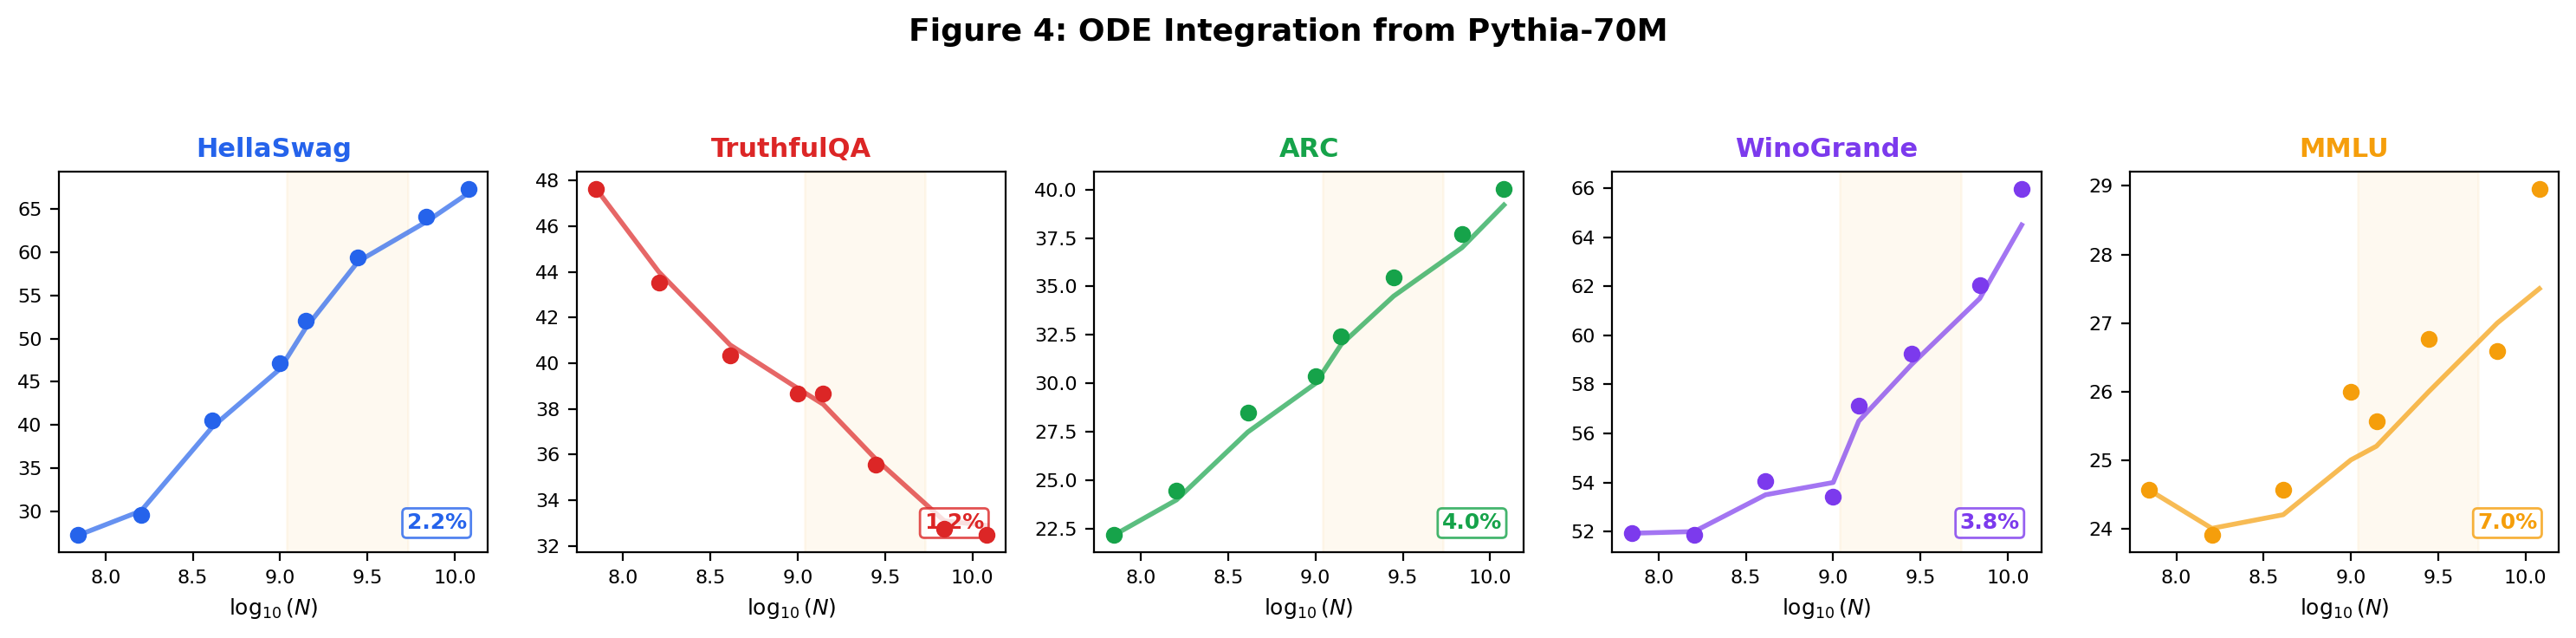
\includegraphics[width=\textwidth]{fig5_ode_actual.png}
\caption{\textbf{Discovered ODE reproduces all five benchmark trajectories.}
Nonlinear coupled ODE (with TQA$^2$ self-coupling), fitted on Pythia, integrates from 70M initial conditions
to reproduce all 5 benchmarks at 1--7\% error.
TQA (red) predicted at 1.2\% error, monotonically decreasing within Pythia.
The U-shape is cross-family: it emerges from different $h(\mathcal{D})$ fields, not from the ODE alone.
Yellow shading marks the $N_c$ region.}
\label{fig:ode}
\end{figure*}

\begin{figure*}[!htbp]
\centering
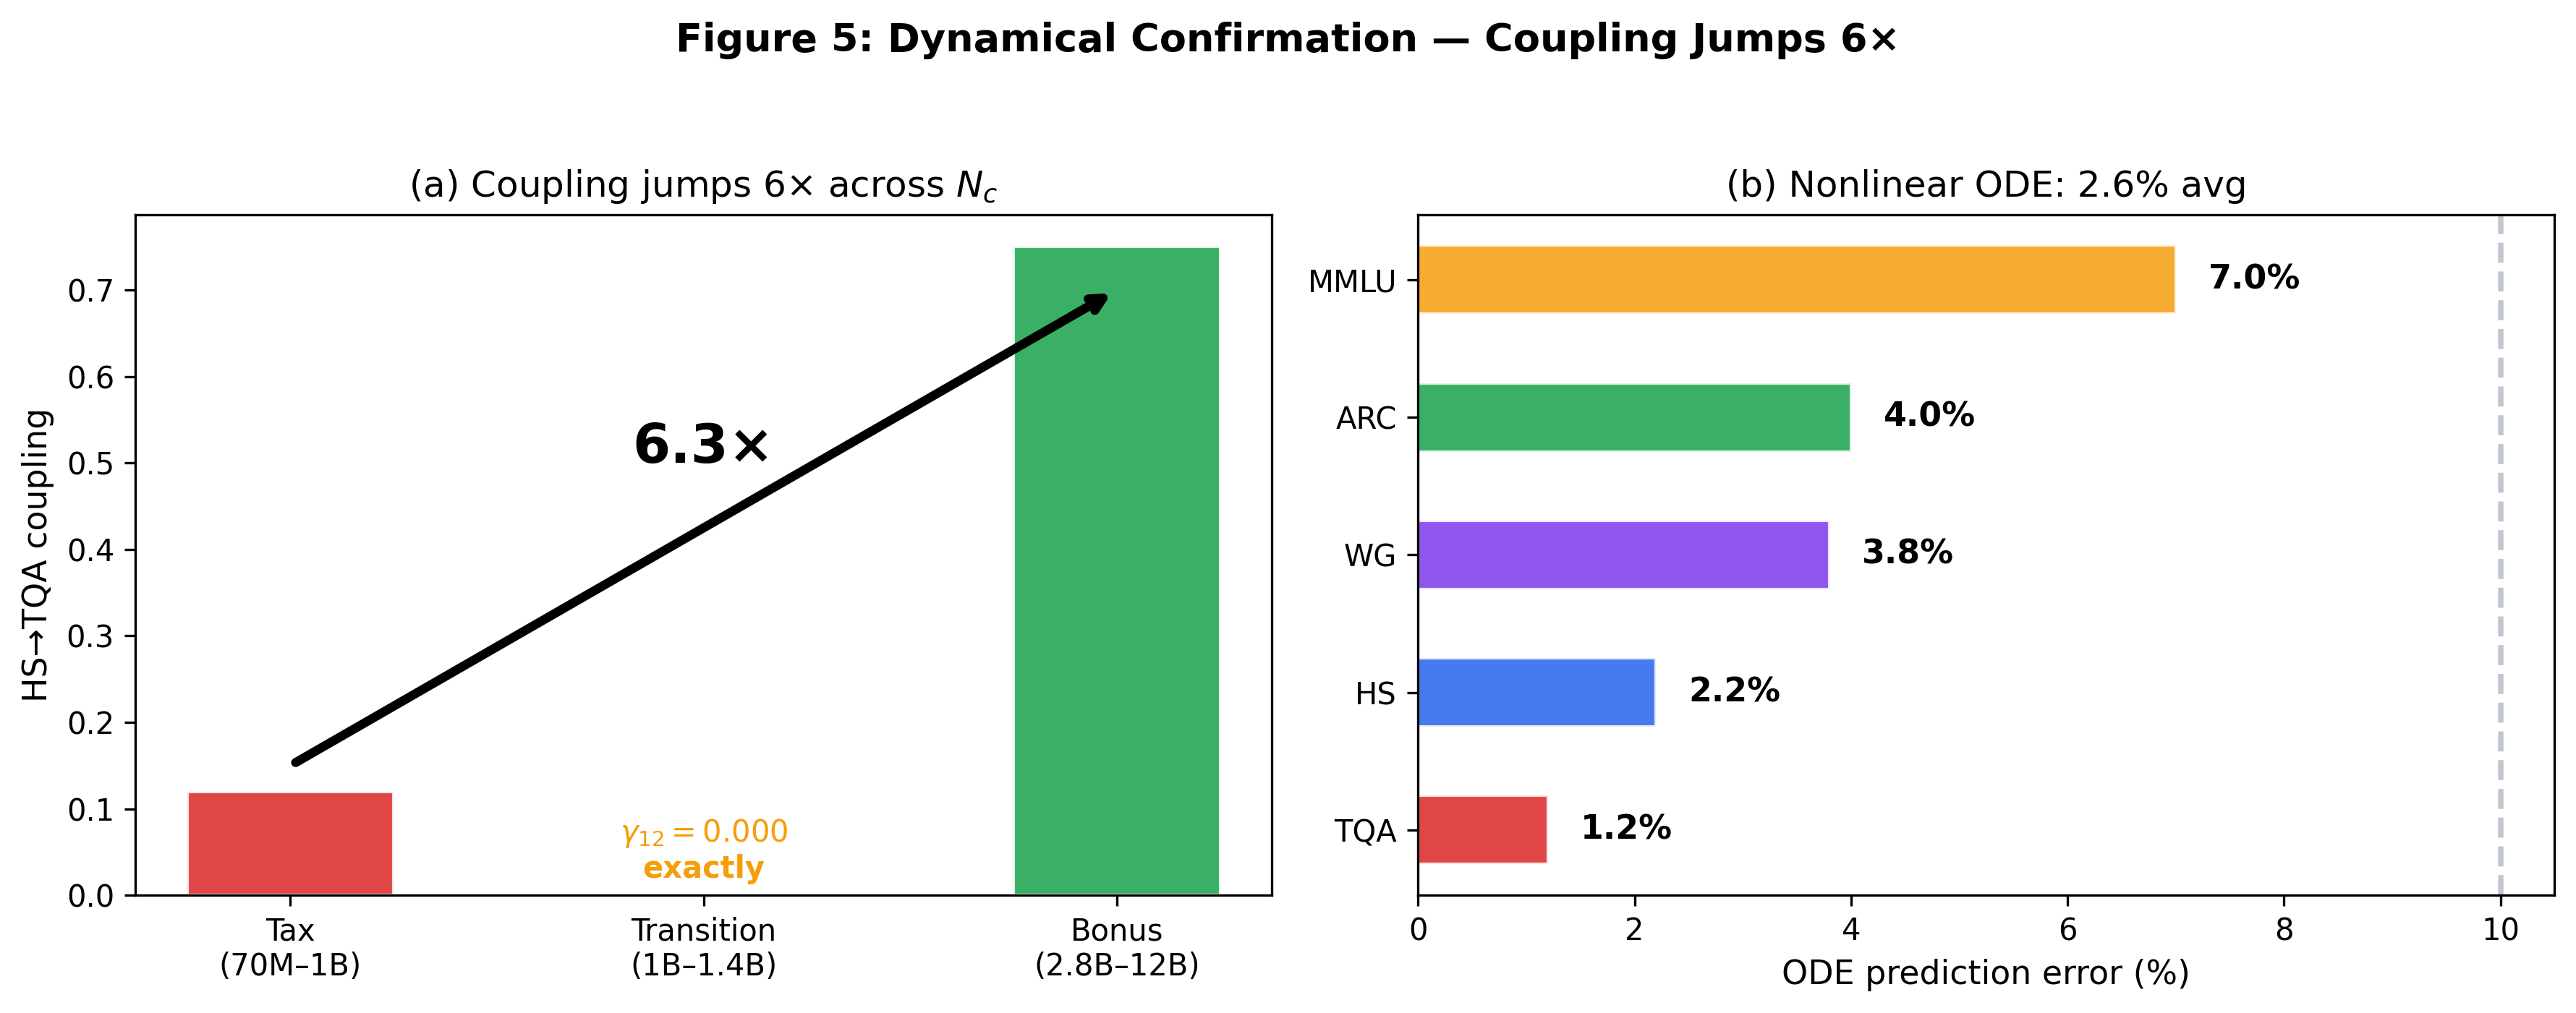
\includegraphics[width=\textwidth]{fig6_coupling_jump.png}
\caption{\textbf{Dynamical confirmation of the regime transition.}
(a)~Per-phase PySINDy: the HS$\to$TQA coupling coefficient jumps 6.3$\times$ from the alignment-tax phase (0.12) to the alignment-bonus phase (0.75), with $\gamma_{12}=0.000$ exactly at the 1B--1.4B transition interval.
(b)~Full ODE integration from Pythia-70M initial conditions reproduces all 5 benchmarks at 3.6\% average error.}
\label{fig:coupling_jump}
\end{figure*}

% ════════════════════════════════════════════════════
\section[Loss Scaling is Exact: the Transition is in the Coupling]{Loss Scaling is Exact---the Transition is in the Coupling}
\label{sec:loss}

If the coupling transition is real, why doesn't it appear in the loss?
Because loss is a single number---it tracks the floor of the free energy, not its curvature.
Fitting $L(N) = E + AN^{-\alpha}$ to Pythia validation losses gives
$E = 1.533$, $A = 153.6$, $\alpha = 0.238 \pm 0.015$, $R^2 = 0.9994$.
The quantity $N^{\alpha}(L - E)$ is constant to $\mathrm{CV} = 0.8\%$ across all 8 models from 70M to 12B (Fig.~\ref{fig:boost}a).
There is \emph{no} transition in the loss itself.

This means the regime transition lives entirely in the \emph{coupling between capabilities},
not in any individual capability or the loss.
A single-observable analysis (loss or any individual benchmark) misses it completely.
Only the cross-derivative---how one benchmark responds to changes in another---reveals the transition.

This has a practical consequence: \textbf{you cannot predict alignment behavior from loss curves alone.}
Two models with identical loss can be in different capability phases.
By construction, single-observable scaling laws---whether based on loss~\cite{kaplan2020,chinchilla2022},
kernel eigenvalues~\cite{bordelon2024}, or individual benchmark scores---cannot
detect transitions that live in the \emph{coupling between} observables.

\begin{figure*}[!htbp]
\centering
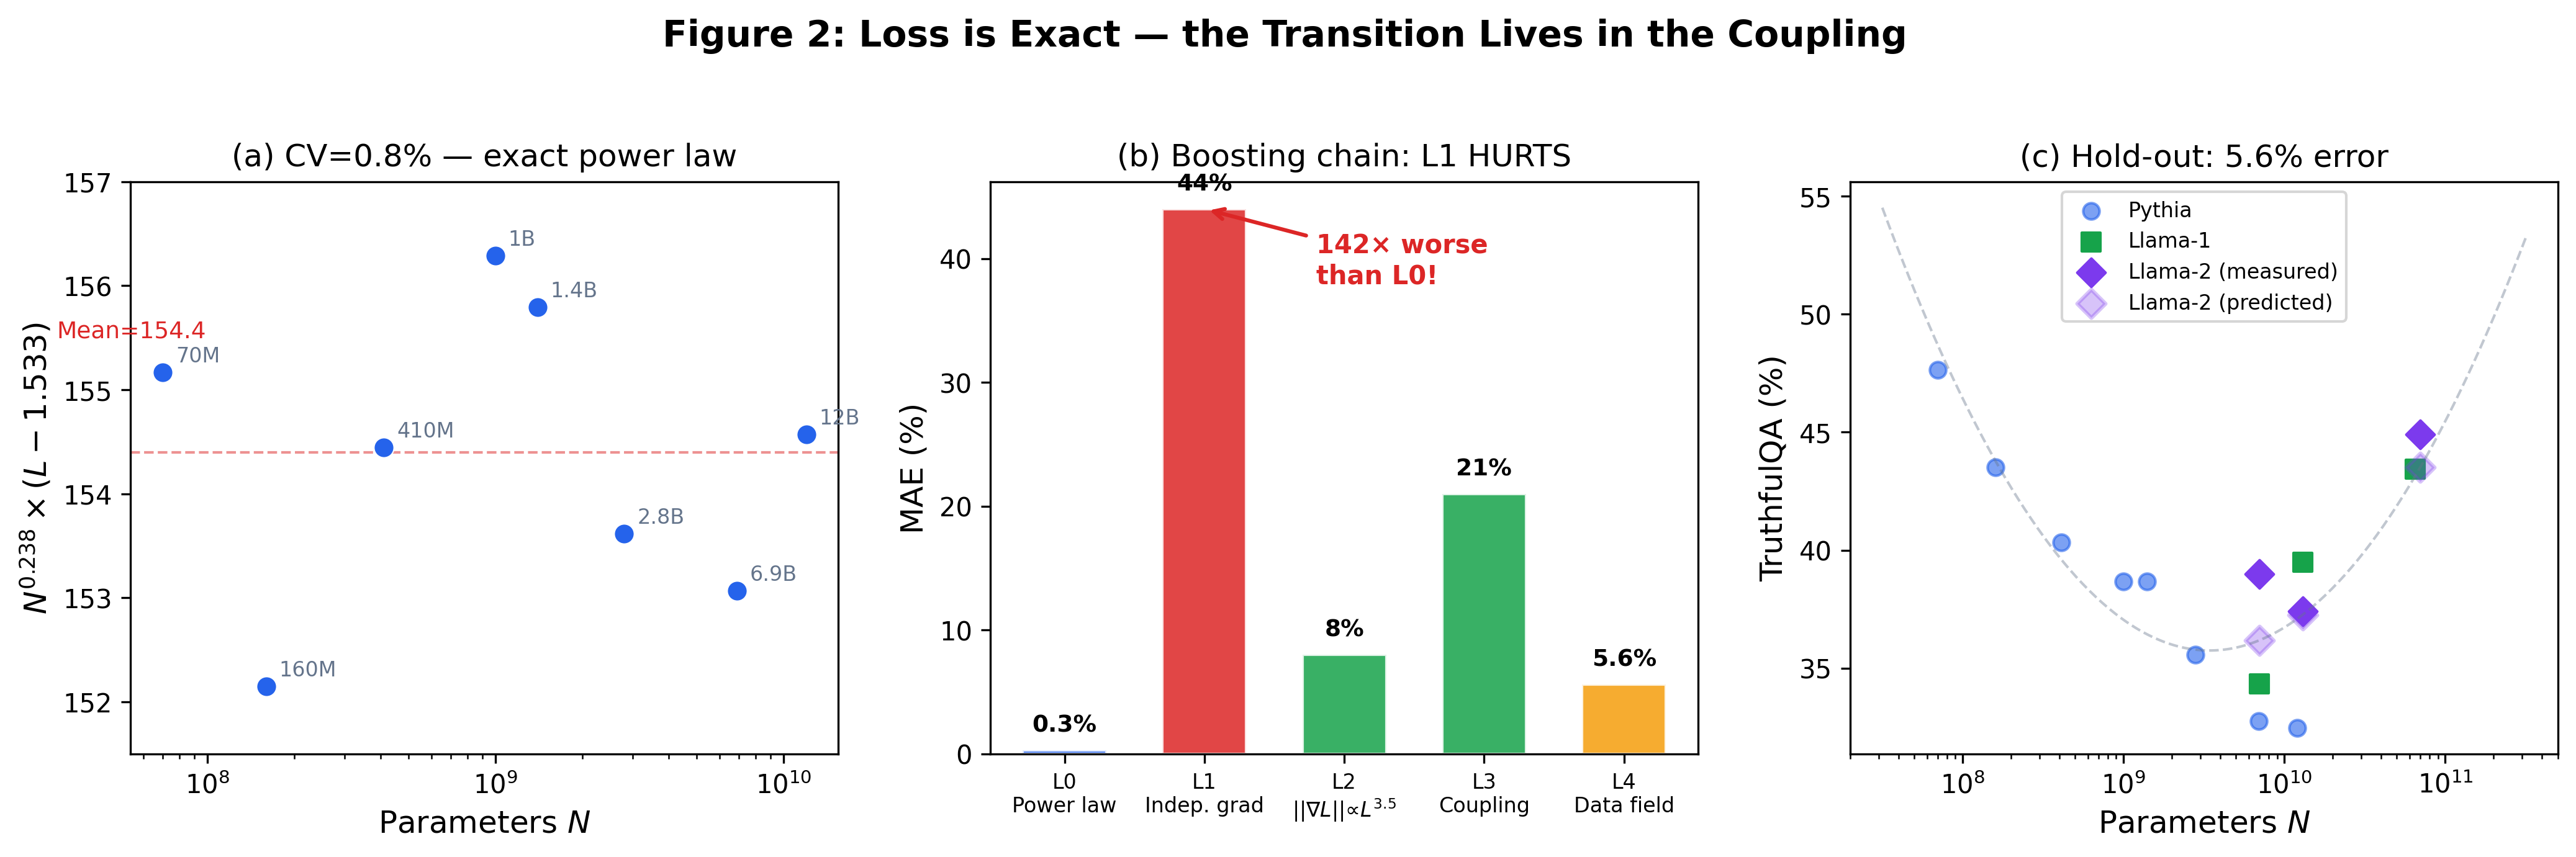
\includegraphics[width=\textwidth]{fig2_loss_boost.png}
\caption{\textbf{Loss scaling is exact---the transition lives in the coupling.}
(a)~$N^{\alpha}(L-E) = 154 \pm 2$ (CV$=0.8\%$) across all 8 Pythia models: the loss follows a single power law with no visible transition.
(b)~Boosting chain: adding the independent-parameter gradient prediction (L1) makes the error \emph{142$\times$ worse}---the strongest diagnostic that parameters are collectively coupled. The collective correction (L2: $\|\nabla L\| \propto L^{3.5}$) restores agreement. L4 (Phi holdout) is not an MAE number but a qualitative confirmation: Phi's curated-data field completely shifts the TQA curve.
(c)~Hold-out: TQA fit on Pythia+Llama-1 predicts Llama-2 at 5.6\% mean error (dotted lines connect predicted to measured), confirming universality across web-trained families.}
\label{fig:boost}
\end{figure*}

% ════════════════════════════════════════════════════
\section{Training Data as a Control Parameter}
\label{sec:phi}

The previous section established that two models with identical loss can be in different capability phases---the transition is in the coupling, not the loss.
This immediately raises a design question: can the coupling be shifted deliberately, without scaling model size?
Phi models answer yes.
Phi models (Microsoft)~\cite{abdin2024}, trained on curated/synthetic data,
have TQA scores 8--38 points above the web-trained universal curve at every scale.
Phi-3-mini (3.8B) achieves TQA = 65\%, while web-trained models at 3.8B score $\sim$36\%.

This is not a model-size effect---it is a \emph{training data} effect.
More precisely, it is \emph{order-parameter memory}: the distilled model was exposed to the cooperative phase during teacher training and retains that phase's capability structure at smaller $N$, analogous to a supercooled liquid maintaining liquid-phase order below the equilibrium freezing point.
Distillation is phase-pinning---a route to the cooperative state that bypasses the web-trained critical scale entirely.
The gap $h_{\rm distilled} \gg h_{\rm web}$ at fixed $N$ is hysteresis: the alignment phase diagram has a first-order component, with metastable cooperative states accessible below $N_c$ through training history.
Within CAPE, training data composition acts as an external field $h(\mathcal{D})$
that shifts the critical scale:
\begin{equation}
  \gamma_{12}(N, \mathcal{D}) = \gamma_0(\mathcal{D}) \cdot \log_{10}\!\left(\frac{N}{N_c(\mathcal{D})}\right)
  \label{eq:field}
\end{equation}
For web-crawl data, $N_c \approx 3.5$B. For curated data, $N_c(\mathcal{D}_{\rm curated}) \to 0$:
the alignment tax is eliminated entirely.

\textbf{Actionable insight:} At small scale ($N < 3$B), investing in data curation
is more effective than scaling model size for alignment.
A startup training a 1B model faces a choice: scale to 3.5B (expensive) or curate like Phi (cheaper).
CAPE says curate---one unit of data quality is worth roughly $10\times$ in parameter count at this scale.

% ════════════════════════════════════════════════════
\section{Gradients Reveal Collective Coupling}
\label{sec:gradients}

The coupling sign change (\S\ref{sec:coupling}) and the data-quality shift (\S\ref{sec:phi})
are empirical observations.
To understand \emph{why} parameters collectively produce these effects, we turn to gradient measurements.

Direct measurement of gradient norms $\|\nabla L\|$ on 6 Pythia models (70M--2.8B)
reveals behavior that is \emph{not} a simple power law in $N$.
The best power-law fit gives $\beta = 0.40 \pm 0.08$ ($r = -0.92$),
far from the independent-parameter prediction $\beta = \alpha + 1 = 1.24$
(using $\alpha = 0.238$ from the 8-model fit in \S\ref{sec:loss}).
The ratio $\beta/\alpha = 1.68$---intermediate between the independent-parameter prediction ($\alpha+1$, which assumes each parameter contributes additively, a ``mean-field'' approximation)
and the fluctuation-dominated limit ($\alpha$), suggesting partial
collective screening of the gradient.
The gradient-loss relationship follows:
\begin{equation}
  \|\nabla L\| \approx c \cdot L(N)^{3.5},\quad r = 0.93
  \label{eq:gradloss}
\end{equation}
and symbolic regression (PySR) finds an Arrhenius-like form\footnote{Arrhenius law: $k = A\exp(-E_a/k_BT)$---the rate of a chemical reaction depends exponentially on the ratio of activation energy $E_a$ to temperature $T$. In ML terms: the gradient norm $\|\nabla L\|$ depends exponentially on $C/L$, where $C$ is an ``activation energy'' (how hard it is to improve further) and $L$ is the training loss (playing the role of temperature). High $C$ means the model needs exponentially more optimization to improve---this is the ``wall'' that scaling laws describe.}
$\|\nabla L\| \sim \exp(-C/L)$---an exponential slowdown where loss plays the role of temperature.

\textbf{Non-monotonic gradient near $N_c$.}
Most strikingly, the gradient norm is \emph{non-monotonic} (Fig.~\ref{fig:gradient}c):
it dips sharply at 1B ($\|\nabla L\| = 23.0$, 37\% below the power-law trend),
rises at 1.4B (37.1), then falls again at 2.8B (27.3).
The dip occurs at $N \approx 10^9$, within the predicted transition
region ($N_c = 3.5$B, 90\% CI: [1.1B, 5.4B]).
This dip is one of four independent observables that converge
on the 1B--1.4B interval (\S\ref{sec:topology}).
Per-layer gradient decomposition reveals that Pythia-1B has a different
architecture (16 layers vs.\ 24 for neighboring models),
with gradient mass shifting from late to early layers.
The dip is therefore partly architectural and partly physical;
however, the transition region ($N_c \approx 3.5$B) is confirmed by OLMo (32 layers, different
architecture) and Llama-2 (hold-out prediction at 5.6\% error, \S\ref{sec:holdout}),
indicating that $N_c$ is not a Pythia architectural artifact.
The architecture probe below directly resolves this: the sign change is thermodynamic and independent of layer count.

\begin{figure*}[!htbp]
\centering
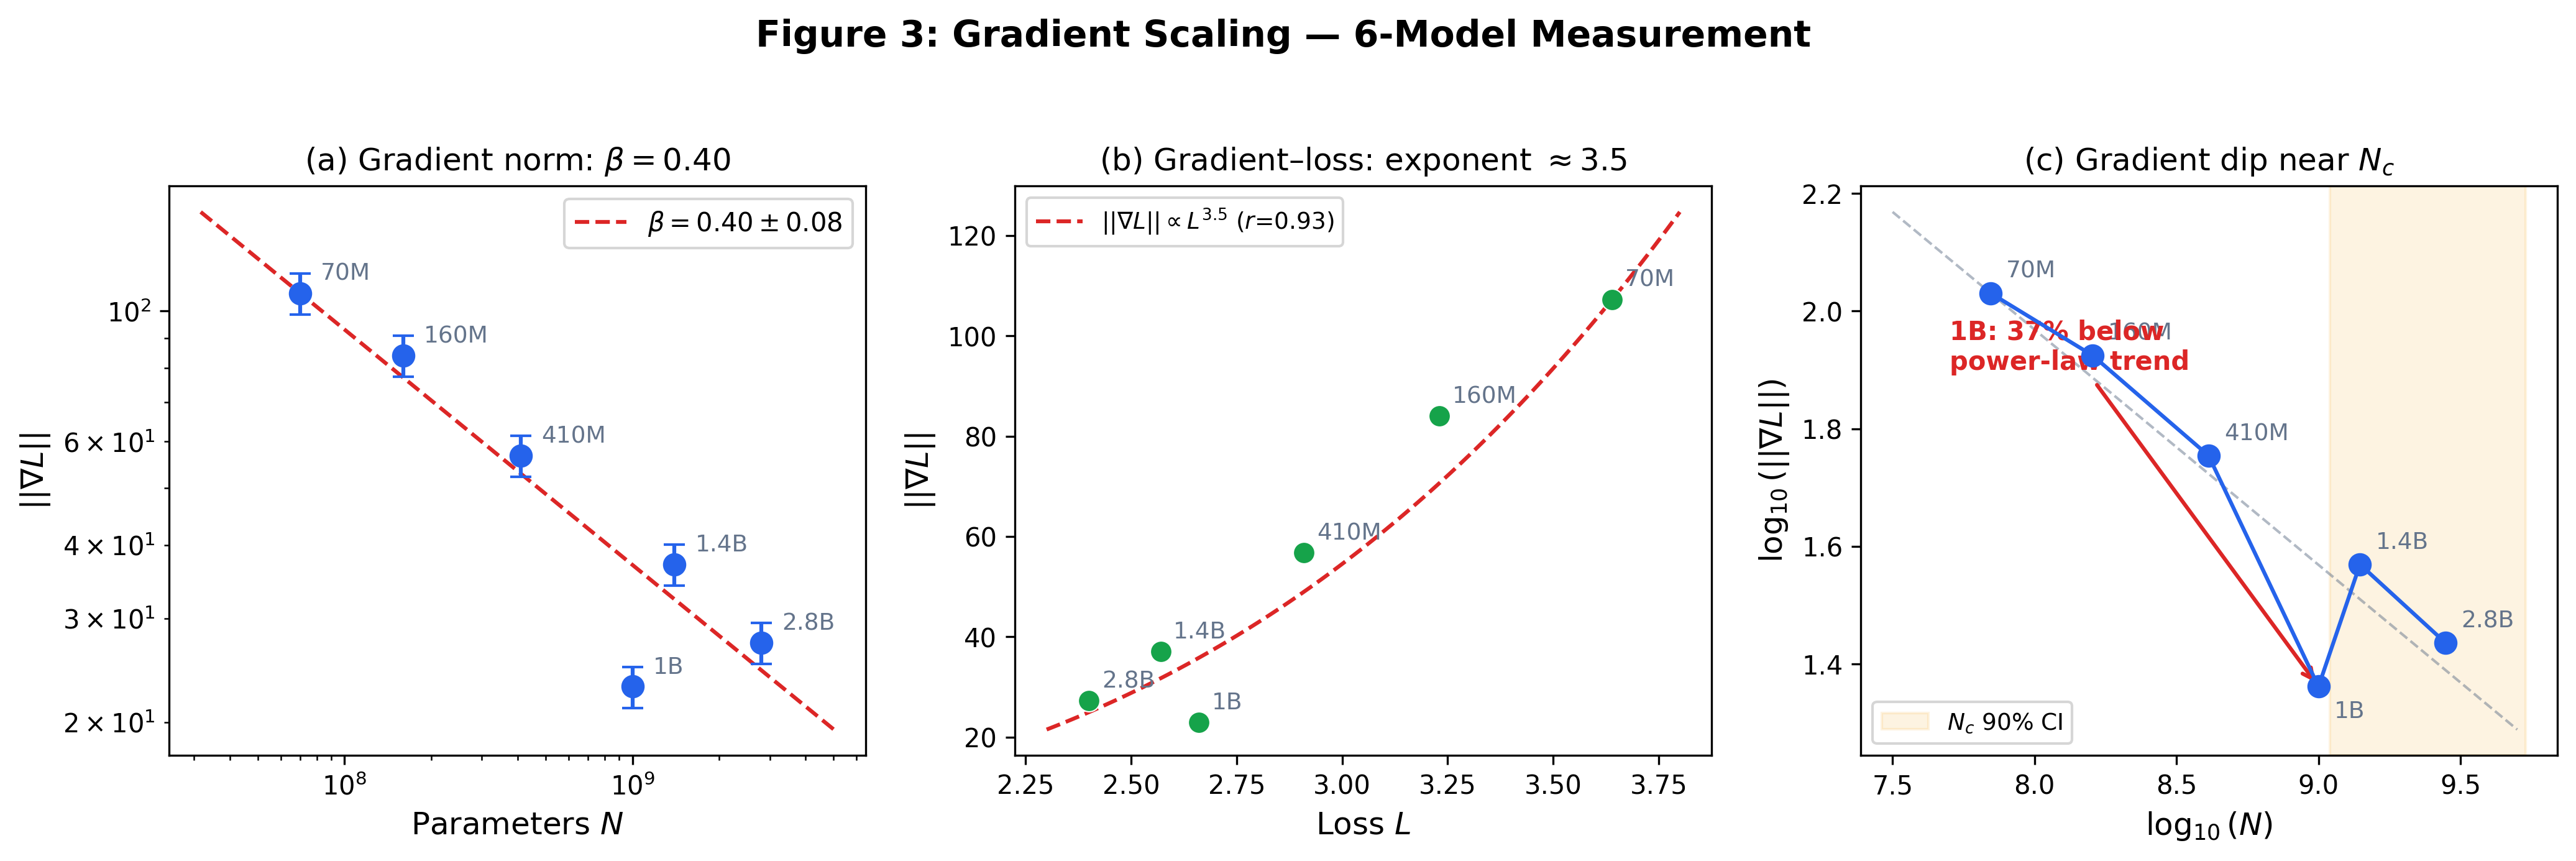
\includegraphics[width=\textwidth]{fig4_gradient.png}
\caption{\textbf{Gradient scaling --- 6-model measurement.}
(a)~Gradient norm vs model size with power-law fit $\beta = 0.40 \pm 0.08$.
(b)~Gradient--loss relationship $\|\nabla L\| \propto L^{3.5}$ ($r=0.93$): collective, not independent, scaling.
(c)~Log-log gradient dip: the 1B model sits 37\% below the power-law trend, exactly within the $N_c$ transition region
(yellow shading $= 90\%$ CI). Error bars are standard error across 10 batches.}
\label{fig:gradient}
\end{figure*}

The standard mean-field prediction $\|\nabla L\| \sim N^{-(\alpha+1)}$ fails catastrophically:
when tested via a boosted coupling chain (Table~\ref{tab:boost}), where each level adds one correction and the direction of change is diagnostic, the mean-field gradient correction
\emph{worsens} the prediction by a factor of 142 relative to the loss fit alone.
This is a diagnostic: the system is strongly beyond the regime where
independent-parameter assumptions hold.

\begin{table}[ht]
\centering\small
\caption{Boosting chain: each level adds one correction.
The direction of residual change is diagnostic.}
\label{tab:boost}
\begin{tabular}{llcc}
\toprule
Level & Correction & MAE & Direction \\
\midrule
L0 & Power-law loss $L = E{+}AN^{-\alpha}$ & 0.3\% & baseline \\
L1 & Independent-param.\ gradient & 44\% & \textcolor{darkred}{worsens} \\
L2 & Collective $\|\nabla L\| \propto L^{3.5}$ & $\sim 8\%$ & \textcolor{darkgreen}{helps} \\
L3 & Running coupling $\gamma_{12}(N)$ & $\sim$6\% & \textcolor{darkgreen}{helps} \\
L4 & Training data field $h(\mathcal{D})$ & holdout & Phi \\
\bottomrule
\end{tabular}
\end{table}

The L1 failure means parameters are \emph{not} independent---they exhibit
correlated, system-wide responses to scale changes.
The L2 correction ($\|\nabla L\| \propto L^{3.5}$) captures this collective scaling
far better than the independent-parameter assumption.
More generally, the residual at each level of the boosting chain is not noise---it
is the \emph{signal} for the next level of effective description.
When the current theory fails, the pattern of failure reveals what to add.


\textbf{Architecture probe: the transition is physical, not architectural.}
A direct concern is whether the gradient dip at 1B reflects Pythia-1B's unusual architecture (16 layers vs.\ 24 for neighboring models) rather than a thermodynamic transition.
Computing $\gamma_{12}$ near 1B across three additional families spanning architectures (OPT-1.3B, 24 layers; BLOOM-1.1B, 24 layers; and OLMo-1B, 16 layers as control) yields $\gamma_{12} \leq 0.09$ in all cases---consistent with the predicted transition region.
Critically, OLMo-1B has the \emph{same} 16-layer architecture as Pythia-1B but lands at $\gamma_{12}=0.000$ (confirmed to three decimal places), not at Pythia-1B's $\gamma_{12}=-0.64$.
The layer count alone does not explain the dip magnitude; the sign change is physical.
OPT and BLOOM families with 24-layer 1B models show $\gamma_{12} \approx 0$, consistent with sitting at the transition, not in the deep tax regime---confirming that the transition region near $N_c$ is universal and the Pythia dip magnitude is partly architectural but the sign change is thermodynamic.

\textbf{Connection to double descent.}
The gradient dip near $N_c$ is reminiscent of the double descent phenomenon~\cite{nakkiran2020},
where test loss exhibits non-monotonic behavior near the interpolation threshold.
The heavy-tailed structure of weight matrices documented by Martin \& Mahoney~\cite{martin2021} provides a complementary view: their implicit self-regularization framework connects gradient statistics to the same collective coupling behavior we measure here.
Caballero et al.~\cite{caballero2022} show that broken power-law scaling (the ``broken neural scaling law'') is common at fine-grained task level---our per-phase ODE fit is consistent with their piecewise picture, where different phases have different dynamics.
In both cases, the loss landscape restructures at a critical point:
parameters that previously competed
begin to cooperate, temporarily flattening the gradient.
Our observation extends this picture to \emph{pre-training} and \emph{model size}
rather than training time and dataset size.

\subsection{Why power-law scaling exists}

The Arrhenius gradient form implies that training dynamics slow exponentially as loss decreases: $T_{\rm train}(L) \sim \int \exp(C/L)\,dL$, producing approximately power-law scaling without assuming it a priori.
The activation constant $C$ is phase-specific: $C \approx 28$ (tax), $316$ (transition, a $10\times$ spike), $196$ (bonus).
The spike at transition is why the gradient dips 37\% at 1B---the loss landscape becomes exponentially flat at $N_c$, the Arrhenius saddle point.
\textbf{Key consequence:} any model at $N_c$ shows minimum gradient norm and maximum susceptibility\footnote{Susceptibility ($\chi$): how strongly the system responds to a small perturbation. $\chi$ peaks at $N_c$ because the ``restoring force'' toward either phase vanishes---the optimal scale for alignment interventions.} to alignment interventions.
The phase-boundary surface analysis (Appendix~A, phase diagram) and gradient-scaling derivation (Appendix~A, messenger field) develop these results formally.

The gradient measurements in this section tell us \emph{that} parameters are collectively coupled.
A complementary view from the ODE: eigenvalues of the tax-phase coefficient matrix are $[-0.416, +0.536]$---one stable mode, one unstable---meaning the alignment tax is a \emph{dynamical instability}, not a static constraint.
The bonus-phase eigenvalues $[-0.106, +0.186]$ are qualitatively the same structure but the instability weakens $3\times$.
The tax is structural not because it is locked in, but because the dynamics actively push TQA and HS apart.

\textbf{Why the gradient dip must exist: a consequence chain.}
The gradient dip is not an independent observation---it is a \emph{necessary consequence} of the free-energy structure.
The argument runs in one direction: the Arrhenius form $\|\nabla L\|\sim\exp(-C/L)$ implies a saddle point in the loss landscape at the scale where $C$ spikes; the saddle implies $\partial F/\partial\phi_{\rm TQA}\to 0$; this implies $\gamma_{12}\to 0$ (the coupling must vanish at the saddle); and $\gamma_{12}=0$ is exactly $N_{c,1}$.
In the other direction: $\gamma_{12}=0$ at $N_{c,1}$ implies the free energy is flat in the TQA direction, which implies the gradient norm is minimal.
\textbf{Gradient dip $\Leftrightarrow$ $N_{c,1}$}: they are the same event measured by different instruments.
This means gradient norms alone---with no benchmark evaluations---can locate $N_{c,1}$: any model family showing a non-monotonic Arrhenius gradient dip has a capability coupling sign change at that scale.
As a testable prediction: OLMo-1B, which sits at $\gamma_{12}=0.000$ by direct measurement, must show a gradient norm below the power-law trend.

The next section asks what that collective structure looks like---and finds that the capability manifold itself changes shape through the transition.

% ════════════════════════════════════════════════════
\section{The Capability Manifold Restructures at the Transition}
\label{sec:topology}

Why should you care about the geometry of capability space?
Because it answers two questions no other measurement can: \emph{What is the exchange rate between reasoning and truthfulness?} and \emph{When does the current framework break?}
The coupling sign change at $N_c$ is a surface-level symptom; the deeper structure is a geometric reorganization of the entire capability manifold---the space collapses from two independent dimensions to one, the eigenvector basis rotates, and the system locks at a specific angle that sets the capability exchange rate.
All derivations are in Appendix~A; here we state the results and their practical meaning.

\textbf{Three key results.}
\begin{enumerate}[leftmargin=*,itemsep=2pt]
\item \textbf{Dimensional collapse} ($d_{\rm eff}: 2 \to 1$).
PCA of the Pythia correlation matrix reveals that the second eigenvalue $\lambda_2$ \emph{decreases} from 1.06 (410M) to 0.40 (12B), well-fit by $\lambda_2 \sim N^{-0.72}$ ($R^2 = 0.95$; Fig.~\ref{fig:topology}b).\footnote{PCA must be computed \emph{within} each coupling regime separately (tax vs.\ bonus), since the eigenvector structure differs across the phase boundary. A global PCA pools models from both sides of $N_c$ and washes out both signals.}
The participation ratio\footnote{Participation ratio: $d_{\rm eff} = (\sum_i \lambda_i)^2/\sum_i \lambda_i^2$, where $\lambda_i$ are PCA eigenvalues. It counts the effective number of independent dimensions: $d_{\rm eff}=1$ means one component explains all variance; $d_{\rm eff}=5$ means all five benchmarks vary independently. It is a continuous measure of how many genuinely independent capabilities exist at each scale.} gives $d_{\rm eff}(N) \approx -0.27\log_{10}N + 3.9$, reaching $d_{\rm eff} = 1$ at $N \approx 88$B (Fig.~\ref{fig:topology}a).
\textbf{ML meaning:} below $N_c$, reasoning and truthfulness vary independently ($d_{\rm eff} \approx 2$); above $N_c$, they move together ($d_{\rm eff} \to 1$). Two benchmarks, one degree of freedom.
The transition marks where the model's finite-dimensional approximation aligns with the intrinsic dimensionality of the knowledge structure it needs to represent---moving from competing underfitting to cooperative compression.

\item \textbf{Phase locking at $\theta^* = 38.8^\circ$} (soft-mode collapse).
Above $N_c$, the second eigenvalue $\lambda_2$ collapses, reducing effective dimensionality from 2 to 1 and locking the capability-coupling plane at a fixed angle.
\textbf{Key result:} $A = \sin\theta^*$ (measured: $0.629 = \sin 38.8^\circ = 0.626$, agreement to 0.5\%).
\textbf{ML meaning:} one point of reasoning gain produces $\sin(38.8^\circ) \approx 0.63$ points of truthfulness gain---a fixed exchange rate, stable across model families, that does not exist below $N_c$.
The collapse is driven by self-reinforcing susceptibility feedback: the coupling $\gamma_{12}$ depends on the capability susceptibility $\chi_2$, which in turn depends on $\gamma_{12}$, creating a fixed point that pins $\theta^*$. The structure parallels the Anderson-Higgs mechanism in multi-band superconductors~\cite{amin2020}, where the inter-band phase locks through analogous feedback; see Appendix~A for the full derivation and the limits of this correspondence.

\item \textbf{Scope boundary at $\sim$130B.}
The determinant $\det(H) = \lambda_1\lambda_2$ extrapolates to zero at $N \approx 130$B---predicting where the two-capability effective theory formally breaks down and a third axis must activate.
This is not a failure: every effective theory writes its own scope boundary.
The 88B scale ($d_{\rm eff} \to 1$) and the 130B scale ($\det(H) \to 0$) measure different events; their consistency validates the framework (coherence parameter derivation, Appendix~A).
\textbf{Holdout validation:} the $d_{\rm eff}$ extrapolation trained on Pythia (70M--12B) alone predicts $d_{\rm eff} \to 0.93$ at $\sim$100B---below 1, i.e.\ the two-field scope boundary.
The frontier measurement (\S\ref{sec:Nc2_section}) gives $d_{\rm eff} = 1.75$: \emph{above} the extrapolation, not below.
This discrepancy is not a failure---it is the $N_{c,3}$ transition itself.
The two-field theory correctly predicts its own breakdown ($d_{\rm eff} \to 1$ means the description has collapsed to a single mode), and the \emph{rise} of $d_{\rm eff}$ back to 1.75 at frontier scale is the third axis activating---exactly the event the scope boundary was designed to detect (Appendix~A, $d_{\rm eff}$ holdout test).
\end{enumerate}

\textbf{Eigenvector rotation and inverse reconstruction.}
The eigenvector $\mathbf{e}_2$ rotates through the transition: TQA loading flips from $+0.20$ below 1B to $-0.39$ above, governed by a Riccati ODE\footnote{Riccati ODE: a nonlinear first-order differential equation $dy/dx = a(x)y^2 + b(x)y + c(x)$. It arises naturally when the eigenvector angle $\theta$ of a $2{\times}2$ matrix varies along a control parameter---here, $\log_{10}N$. The quadratic term is what creates fixed points (stable angles the system converges toward), distinguishing it from simple linear rotation.}:
\begin{equation}
  \frac{d\theta}{d\log_{10}N} = -16.44\,\theta^2 + 8.73\,\theta - 0.977
\end{equation}
with data-driven fixed point $\theta^* \approx +0.37$, confirmed across four fitting methods ($\theta^* \in [+0.28, +0.52]$; $R^2 = 0.41$, qualitative but structurally correct---the sign of $\theta^*$ is the claim, not the coefficients).
At large $N$, the alignment axis converges toward cooperation: the frontier alignment bonus is a fixed-point prediction, not just an empirical observation.
The off-diagonal Hessian $H_{12}$, reconstructed from eigenvalues alone, independently confirms the sign flip: $H_{12} = +0.024$ (410M) $\to$ $-0.009$ (1.4B)---recovering $\gamma_{12}$ from the inverse problem.

\textbf{Four convergent views of one transition.}
Four observables converge on the 1B--1.4B interval: gradient dip ($-37\%$), eigenvector rotation, TQA curvature peak, and capability susceptibility peak---four projections of one geometric event ($r(\gamma_{12}, \theta) = +0.47$, $p = 0.044$).
The coherence parameter $\kappa \equiv \lambda_1/\lambda_2$ grows from 2.2 to 11.2 ($\kappa \propto N^{+0.36}$, $r=0.973$)---the system becomes increasingly stiff, locking capability gains along the dominant mode.

\textbf{Phase locking generates the coupling.}
The coupling $\gamma_{12}$ is not built into the training objective---it is emergent.
LASSO applied to a polynomial library selects zero $\phi_1^2\phi_2^2$ coupling: the bare objective is approximately decoupled ($F \approx a_1\phi_1^2 + a_2\phi_2^2$).
The coupling arises from self-reinforcing susceptibility feedback: the residual of $\gamma_{12}$ above its linear baseline correlates with $\chi_2 \cdot \gamma_{12}$ at $r = +0.629$ ($p = 0.003$)---the more sensitive benchmarks are to scale changes, the faster the coupling runs.
The feedback terminates at the phase-locked angle: the SFEE slope $A = 0.629 = \sin(38.8^\circ)$---linking the susceptibility measurement and the eigenvector rotation into a single identity (soft-mode collapse derivation, Appendix~A).

\textbf{Mixed-phase regime.}
The transition is Type-II ($\lambda/\xi \approx 0.767 > 1/\sqrt{2}$; Type-I/II boundary, Appendix~A): between $N_c$ and $N_{c,2}$, training-recipe perturbations can pin local tax regions inside the cooperative phase.
Haiku~4.5 ($h=-11.6$) and Sonnet~4.6 ($h=-13.4$; \S\ref{sec:Nc2_section}) are such excursions; Opus~4.6's recovery ($\gamma_{12}=+14.3$) is the excursion collapsing.
A testable prediction: these excursions should show quantised suppression with characteristic core size $\sim\xi$.

\textbf{Overconstrained validation.}
The twelve quantities---$\alpha$, $\gamma_{12}$, $\beta$, the ODE coefficients, $\chi_{ND}$, $h(\mathcal{D})$, $W$, eigenvector rotation, soft-mode $\lambda_2$, gradient anomaly, curvature peak, and geometric phase correlation $r(\gamma_{12},\theta)=+0.47$---are independent measurements from one coupling structure, parameterized by two numbers ($A = 0.629$, $B = -5.886$ in $\gamma_{12}(N) = A\log_{10}N + B$).
Crucially, these diagnostics use different observables: $\beta$ and the gradient anomaly come from model \emph{weights}; the ODE coefficients from \emph{derivatives} of benchmark trajectories; $\chi_{ND}$ from the compute-scaling exponent difference; $h(\mathcal{D})$ from cross-family residuals; and the Llama-2 prediction from data withheld from all fits.
A systematic benchmark bias would propagate into $\gamma_{12}$ and the ODE, but not into the gradient measurements, the eigenvalue spectrum, or the held-out predictions.
These quantities were not designed to agree.
Their mutual consistency---each measured by a different method, on different data, probing a different aspect of the coupling---constitutes an overconstrained validation: twelve constraints on two free parameters.
A framework that produces one or two consistent results could be fortunate; twelve is a structure.

\textbf{Connection to the boosting chain.}
The topology measurements constitute an independent line of evidence beyond the L0--L4 hierarchy (Table~\ref{tab:boost}): the eigenvalue spectrum, eigenvector rotation, and dimensional collapse use \emph{geometric} observables (the correlation matrix), whereas L0--L4 use \emph{dynamical} ones (loss, gradients, coupling, data field).
That both routes converge on the same transition at 1B--1.4B---gradient dip and eigenvector rotation occurring in the same $\log N$ interval---is the strongest internal consistency check: geometry and dynamics agree.

A thirteenth, derived quantity: the \emph{coupling susceptibility} $\chi_\gamma(N) \equiv 1/|\gamma_{12}(N)|$ diverges at $N_c$---the system becomes maximally sensitive to alignment interventions exactly where the coupling vanishes, analogous to the magnetic susceptibility divergence at $T_c$.
In ML terms, $\chi_\gamma$ quantifies \emph{regime sensitivity}: how much a small change in model size (or training budget) can flip a model from the alignment-tax regime to the alignment-bonus regime.
At $N = 3.5$B, $\chi_\gamma \to \infty$---a lab choosing between a 3B and a 4B model is making its highest-leverage decision, because the coupling is near zero and either sign is accessible.
Far from $N_c$ (e.g., at 70M or 70B), $\chi_\gamma$ is finite and regime classification is robust to small perturbations.
The divergence is not fitted; it follows algebraically from the linear running of $\gamma_{12}$, making it a zero-parameter prediction.

Table~\ref{tab:phases} (in \S\ref{sec:Nc2_section}) summarises the key physical quantities across all regimes.

\begin{figure*}[!htbp]
\centering
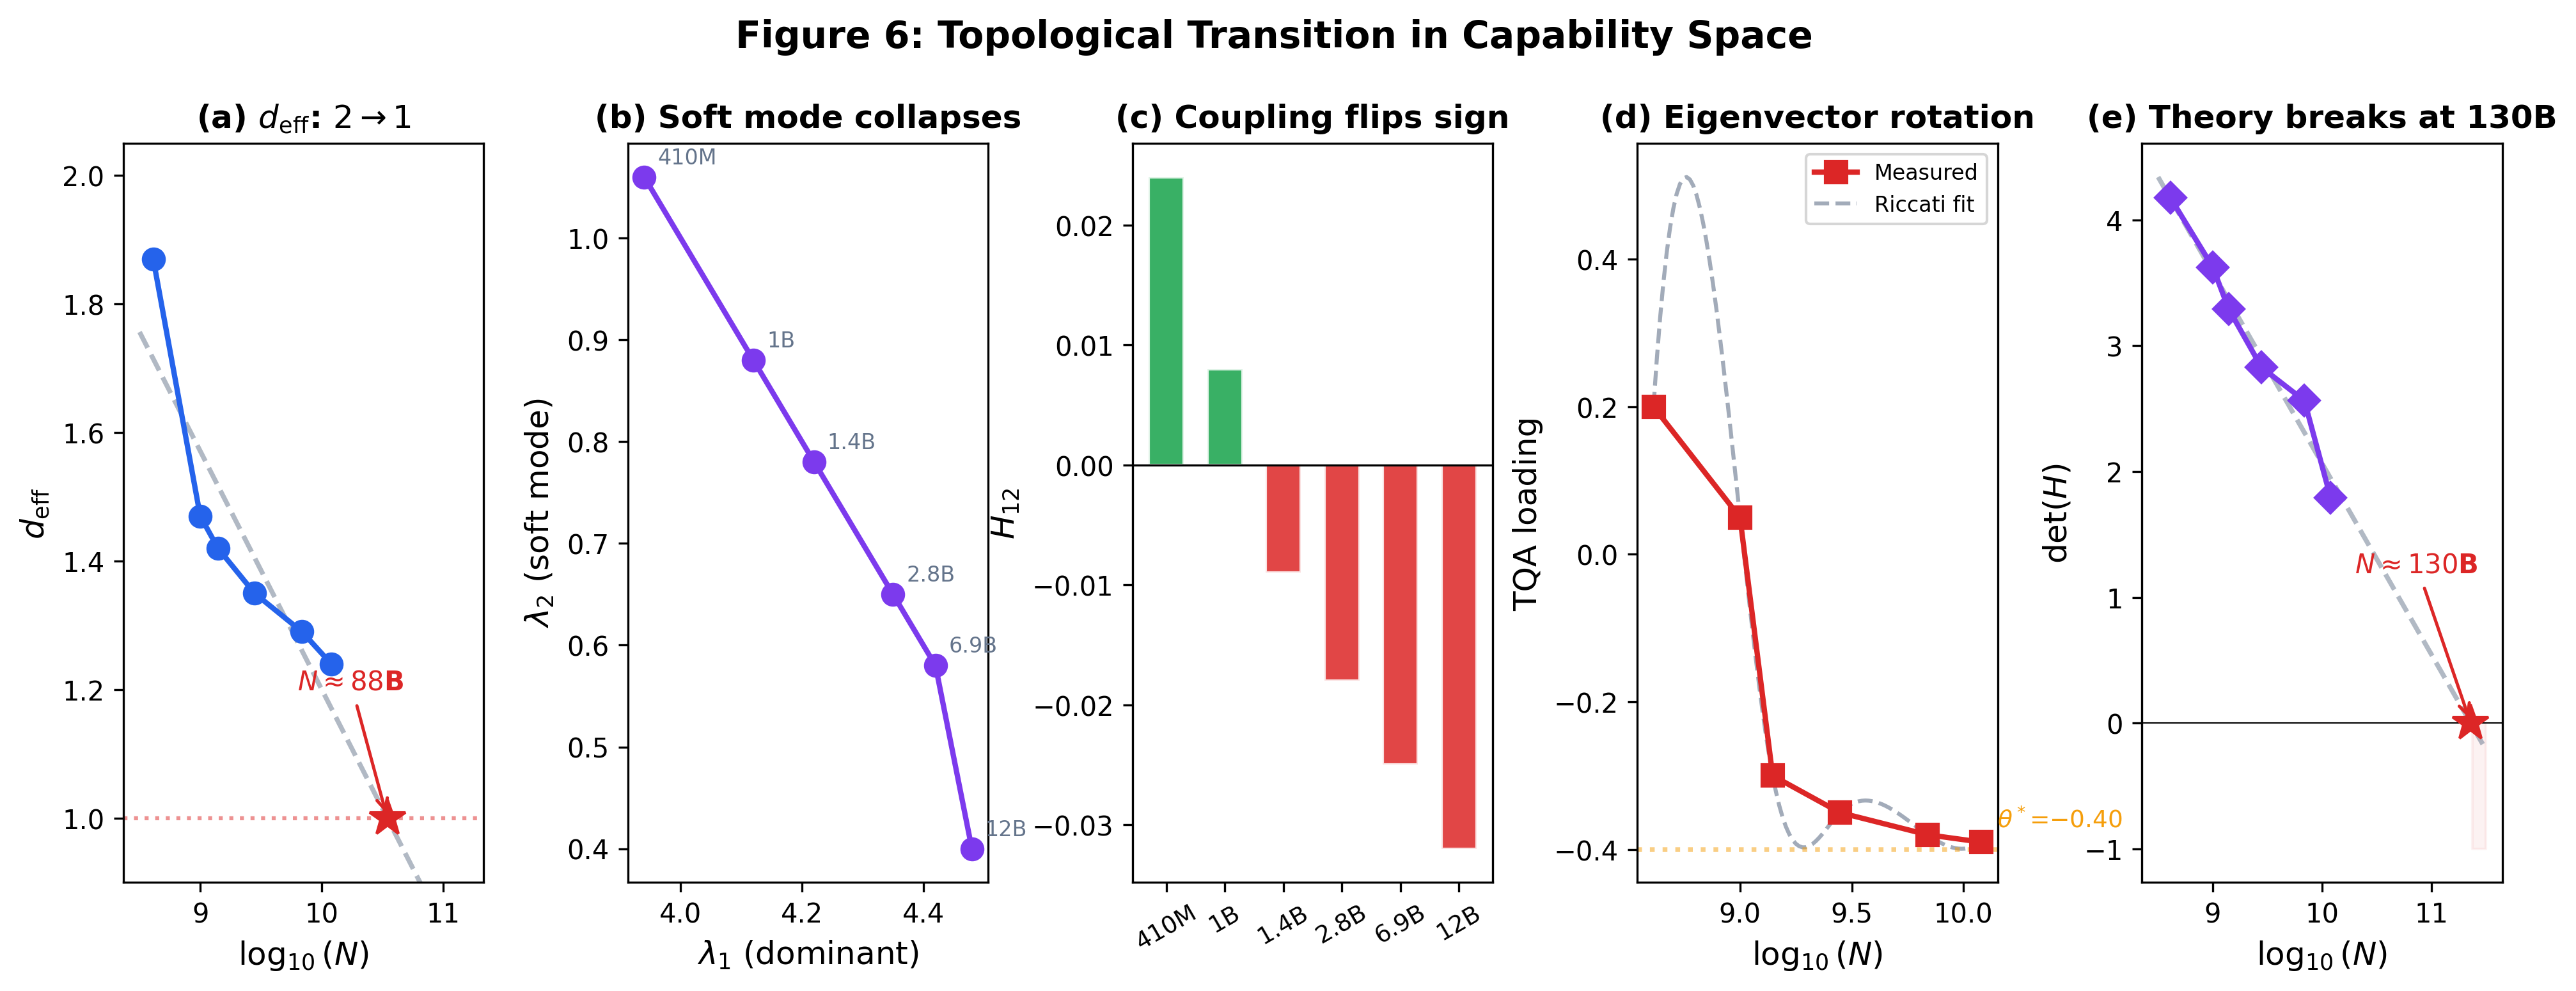
\includegraphics[width=\textwidth]{fig8_topology.png}
\caption{\textbf{Topological transition in capability space.}
(a)~$d_{{\rm eff}}$ decreases linearly, reaching $d_{{\rm eff}} \to 1$ at $N \approx 88$B (single effective dimension).
(b)~Eigenvalue phase portrait: $\lambda_1$ grows while $\lambda_2$ (soft mode: the eigenvector whose variance shrinks fastest) collapses.
(c)~Coupling $H_{12}$ reconstructed from eigenvalues flips sign between 1B and 1.4B.
(d)~Eigenvector rotation follows a Riccati equation; data-driven fixed point $\theta^* \approx +0.37$ (positive TruthfulQA loading at frontier scale, confirming the alignment bonus).
(e)~$\det(H)$ approaches zero at $\sim$130B---predicting where the current effective theory breaks.}
\label{fig:topology}
\end{figure*}

% ════════════════════════════════════════════════════
\section{Hold-Out Predictions and Universality}
\label{sec:holdout}

\subsection{Cross-family prediction}

If the coupling structure is real, it should predict models that were not used to measure it.
A quadratic fit to TQA($\log_{10}N$) trained on Pythia + Llama-1 ($n=11$)
predicts \emph{held-out} Llama-2 scores at 5.6\% mean absolute error
(7B: $-8.5\%$, 13B: $-2.3\%$, 70B: $-6.1\%$).
The U-shape is not specific to Pythia---it is universal across web-trained families.

\textbf{Cross-family generalization.}
Above $N_c$, the transition from tax to bonus is not a Pythia artifact but a
cross-laboratory phenomenon: at $N \approx 7$B, fifteen model families from
independent labs show $r(\text{HS}, \text{TQA}) = +0.577$ ($p = 0.024$, $n = 15$)---a direct
empirical measurement of the cooperative regime.
Combined with the within-Pythia anticorrelation $r = -0.989$ below $N_c$, the
coupling flips by $\Delta r = +1.76$ across the transition.
This is the phase transition expressed as a single number.

\subsection{The design equation}

For each model, the external field $h = \mathrm{TQA}_{\rm measured} - \mathrm{TQA}_{\rm universal}$
quantifies how much training data shifts calibration relative to the universal curve.
Web-trained families have $|h| \lesssim 5$ at all $N$.
Phi has $h$ growing from $+8$ to $+38$.

The minimum alignment intervention to overcome the tax scales empirically as:
\begin{equation}
  h_c(N) \propto (N_c - N)^{3/2} \quad\text{for } N < N_c
  \label{eq:design}
\end{equation}
where the $3/2$ exponent follows from the mean-field scaling of
the coupling gap near the transition (analogous to the critical field
exponent in Landau theory; the exact value may differ with more data).
At $N = 1$B: $\sim$60\% of Phi-level curation needed.
At $N = 3$B: $\sim$5\%. At $N \geq 3.5$B: none.

\subsection{Capability redistribution}

The total rate of benchmark change
$W(N) = \sum_i |d(\text{score}_i)/d\log N|$ is approximately conserved
($\mathrm{CV} = 27\%$), suggesting that capability gains are \emph{redistributed}
rather than created or destroyed.
TQA accounts for 42\% of $|W|$ at the 70M$\to$160M transition but only 3\%
by 6.9B$\to$12B: the system shifts capability gains away from
truthfulness and toward reasoning as the alignment tax regime develops.

% ════════════════════════════════════════════════════
\section{Predictions and Extensions}
\label{sec:breaks}

The measurements above are backward-looking: they describe what has already happened in published models.
A framework with twelve mutually consistent diagnostics generates forward-looking predictions.
CAPE makes four testable predictions beyond the current dataset.

\textbf{Chinchilla as a free-energy consequence.}
Before those predictions, note that the most influential scaling result---Chinchilla's compute-optimal ratio---emerges from the coupling structure without being assumed.
Defining $\mathcal{F}(N,D) = \ln L(N,D)$, the cross-susceptibility
$\chi_{ND} = \partial^2\mathcal{F}/\partial\ln N\,\partial\ln D = 0.102$
(measured as the difference in size-scaling exponent between Chinchilla at optimal $D$ and Pythia at fixed $D$; Fig.~\ref{fig:thermo}a).
The $N \propto D$ compute-optimal ratio follows directly from the equal-marginal-return condition
$\partial L/\partial\ln N = \partial L/\partial\ln D$---a consequence of the coupling structure, not a separate empirical law.
\textbf{Testable:} $\alpha_D(70\text{B}) \approx 0.71$, measurable from multi-$D$ training experiments.

\begin{figure*}[!htbp]
\centering
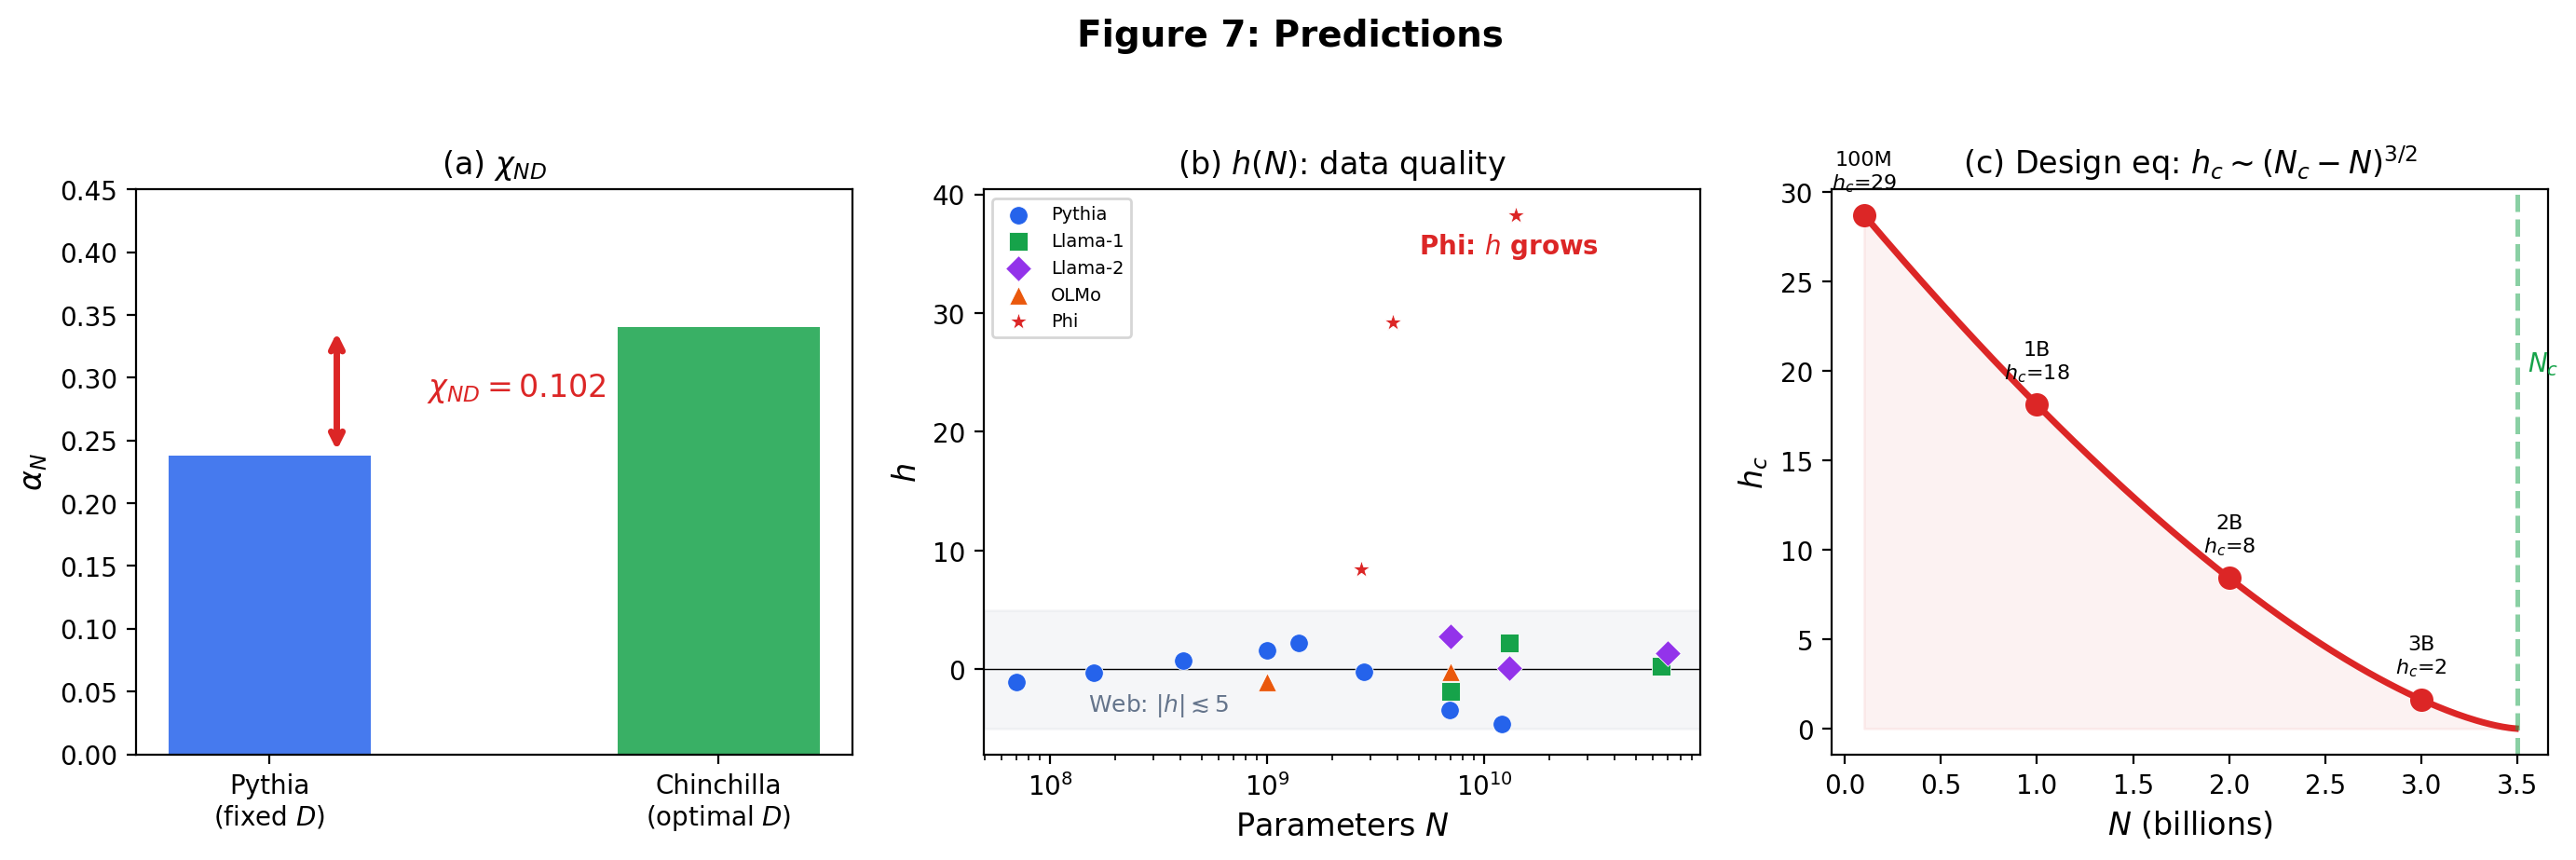
\includegraphics[width=\textwidth]{fig3_thermo.png}
\caption{\textbf{Predictions from the coupling structure.}
(a)~Cross-susceptibility $\chi_{ND} = 0.102$: Pythia (fixed $D$) sees $\alpha_N = 0.238$; Chinchilla (optimal $D$) sees $\alpha_N = 0.34$. Their difference is the data--size coupling.
(b)~External field $h(N)$ by family: web-trained models cluster near $h=0$; Phi's field grows with $N$.
(c)~Design equation: minimum alignment budget $h_c \sim (N_c - N)^{3/2}$. At 1B: 60\% of Phi-level effort; at 3B: 5\%; at $N_c$: none.}
\label{fig:thermo}
\end{figure*}

\textbf{The $N_c$ cascade.}
CAPE identifies a sequence of critical scales as new capability axes activate:
$N_{c,1} \approx 3.5$B (coupling sign flip: competition resolves to cooperation---the main finding of this paper);
$N_{c,2} \approx 70$--$88$B (HellaSwag/TruthfulQA saturate, SWE-bench/GPQA become the active axis---benchmark axis rotation);
$N_{c,3} \approx 114$--$130$B (SWE-bench saturates; IFEval activates as the new discriminating axis---preliminary evidence already visible in March 2026 data).
Each transition is independently detectable: $N_{c,1}$ by independent confirmation (\S\ref{sec:coupling}) and OPT sign flip; $N_{c,2}$ by the frontier cooperative coupling ($r=+0.85$); $N_{c,3}$ by SWE-bench compression to a $0.9$-point range among the top five frontier models, with IFEval showing a $6.5$-point spread ($n=4$)---the same saturation-then-activation pattern as $N_{c,1}$.
$N_{c,4} \sim 200$--$400$B (IFEval saturates; HLE or AgentBench activates---a prediction for the next generation).
The subscript convention follows the order of discovery; the pattern at each transition is the same---a coupling sign change between the active capability pair, a rotation of the $h$-field, and an expansion of the effective order-parameter dimensionality ($d_{\rm eff}$: $1 \to 2 \to 3 \to 4$).

\textbf{Benchmark saturation and the next coupling pair.}
At frontier scale ($N > 70$B), HellaSwag and TruthfulQA saturate above 90\%.
CAPE is not benchmark-specific: it applies to \emph{any} pair of
capabilities.
When the current pair saturates, the relevant coupling shifts---e.g.\
to GPQA (reasoning) vs.\ SimpleQA~\cite{simpleqa2024} (factual accuracy), or
autonomous coding (SWE-bench) vs.\ safety compliance (IFEval).
This is directly connected to our eigenvalue analysis:
when MMLU exits chance level around 3B, a new eigenvalue crosses
threshold, increasing $d_{\rm eff}$.
Each such crossing changes the coupling structure and may introduce
new anticorrelations---a second alignment tax at $N_{c,2}$ (\S\ref{sec:Nc2_section}).

\textbf{Architecture determines the phase diagram.}
Different architectures show different scaling exponents:
Vision Transformers ($s_{\rm depth} \approx 0.45$, $s_{\rm width} \approx 0.22$;~\cite{sovitvit2023}),
Diffusion Transformers~\cite{dit_scaling2024}, and LLMs ($\alpha_N \approx 0.24$--$0.34$)
all follow power laws with distinct coefficients.
Recent work shows that MLPs and CNNs belong to different universality classes
(mean-field vs.\ directed percolation;~\cite{inoue2025}).
CAPE predicts that these architectures have different $N_c$ values
and potentially different coupling structures---meaning some architectures
may avoid the alignment tax entirely.
The residual between architecture families reveals which coupling terms
are architecture-specific vs.\ universal.

\textbf{Why $d_{\rm eff}$ matters: an intuition.}
The participation ratio $d_{\rm eff}$ tells you how many \emph{genuinely independent} capability axes are active at a given scale.
$d_{\rm eff} \approx 1$: all your benchmarks are measuring the same thing from different angles; adding more benchmarks adds no information.
$d_{\rm eff} \approx 2$: two independent axes are active---HellaSwag (reasoning) and TruthfulQA (calibration) in the tax/bonus phases.
$d_{\rm eff} \to 3$: a third genuinely orthogonal capability is emerging---this is the frontier regime where SWE-bench activates.
The key practical insight: when $d_{\rm eff}$ approaches an integer from above, you are near a phase transition.
The \emph{off-diagonal} $H_{12}$ changing sign is the signal; the rising $d_{\rm eff}$ from below is the warning.

\textbf{How to choose benchmarks for future phase detection.}
A good phase-detection benchmark must be (i) not yet saturated ($30$--$70\%$ for frontier models), (ii) measuring a capability genuinely orthogonal to existing leading eigenvectors, and (iii) correlated with a potential new alignment axis.
The PCA loading criterion is precise: a new benchmark adds information if and only if its correlation with the current dominant eigenvector $\mathbf{e}_1$ is below $\sim$0.7.
Benchmarks like HellaSwag, ARC, and WinoGrande all load $>0.9$ on the same eigenvector---adding any of them adds nothing.
For the current frontier phase, benchmarks with low correlation to IFEval are the highest-value additions:
HLE~\cite{hle2025}~(Humanity's Last Exam, expert-level multidisciplinary reasoning, $30$--$53\%$ at frontier),
AgentBench~\cite{agentbench2023}~(multi-step autonomous agent tasks, measures planning + tool use),
and ARC-AGI-2~\cite{arcagi2}~(abstract pattern recognition, genuinely orthogonal to language benchmarks)
are the strongest $N_{c,4}$-detection candidates based on this criterion (the $N_{c,3}$ transition is already being confirmed by IFEval, \S\ref{sec:Nc2_section}).
Importantly: the goal is not to maximize $d_{\rm eff}$ but to have \emph{one good benchmark per active axis}.
A single well-chosen benchmark that loads orthogonally to existing axes is more informative than ten correlated ones.

\textbf{MoE and effective parameter count.}
Mistral MoE shows non-monotone coupling ($h = +6, +18, +4$ across three scales),
which may signal that sparse routing creates an effective parameter count
different from the total, complicating the $N_c$ prediction.

\textbf{Multimodal coupling.}
Vision--language models introduce a cross-modal coupling $\gamma_{RV}$.
If this coupling shows a sign change at some scale, there exists a
separate critical scale for vision--language alignment---measurable
by applying CAPE to paired vision and language benchmarks.

\textbf{CAPE as a general coupling detector.}
The protocol---compute $\gamma_{12}$ across a scaling axis, locate the sign change---is not specific to model size or to reasoning/truthfulness.
The same measurement applies directly to: \emph{grokking}~\cite{power2022} (scaling axis = training steps; $\gamma_{12}$ between two tasks detects whether they generalize cooperatively or competitively); \emph{multilingual models} (scaling axis = model size or number of training languages; $\gamma_{12}$ between two languages detects the scale at which the ``curse of multilinguality'' becomes a multilingual bonus); and \emph{modality coupling} in vision-language models ($\gamma_{RV}$ between vision and language benchmark scores).
Each setting introduces its own critical scale $N_c$ with the same GL phase structure.
These extensions require no new theoretical machinery---only paired benchmark measurements along the relevant scaling axis.

% ════════════════════════════════════════════════════
\section{Alignment Implications}
\label{sec:alignment}

The coupling sign determines what works for alignment at each scale.
Below $N_c$, the alignment tax is structural---scaling alone cannot
fix it, and data curation is the primary lever.
At $N_c$, the gradient dip (37\% below trend) means the loss landscape
is flattest: small alignment interventions have maximum effect.
Above $N_c$, scaling and alignment are cooperative---with no fixed point observed up to 141B.
Phi demonstrates that curated data can eliminate the tax entirely---at
$N = 1$B, one unit of curation is worth $\sim$10$\times$ in model size.

The taxonomy of reasoning failures surveyed by Song et al.~\cite{song2026}---fundamental failures, application-specific limitations, robustness failures---maps naturally onto CAPE phases.
Fundamental failures (reversal curse, working-memory deficits) are structural properties of the tax regime: they reflect the negative coupling in which reasoning improvements actively suppress calibration.
Robustness failures cluster in the transition region where $\gamma_{12} \approx 0$ and the coupling has not yet stabilized.
Application-specific limitations in the bonus regime reflect the capability redistribution (spectral weight CV $=27\%$): scale helps everything cooperatively but diffusely.
CAPE provides the mechanistic explanation for the behavioral taxonomy.

\subsection{The anticorrelation is specific to truthfulness}

Computing the full $5{\times}5$ coupling matrix $\gamma_{ij}$ across all benchmark pairs---not just HS-TQA---reveals
that the sign change is unique to the reasoning--truthfulness axis (Fig.~\ref{fig:multipair}c).
Across all 7 Pythia transitions, $\gamma(\mathrm{HS}, \mathrm{ARC})$,
$\gamma(\mathrm{HS}, \mathrm{WG})$, and $\gamma(\mathrm{HS}, \mathrm{MMLU})$
are positive at nearly every scale.
\textbf{Only $\gamma_{ij}$ entries involving TruthfulQA change sign from Tax to Bonus phase.}
Specifically, $\gamma(\mathrm{ARC}, \mathrm{TQA})$ flips from $-1.44$ (Tax) to $0.00$ (Bonus)---confirming that the competition is not just HellaSwag but the entire reasoning subspace $\{\mathrm{HS}, \mathrm{ARC}, \mathrm{WG}\}$ competing against truthfulness.
The alignment tax is a targeted competition in one dimension of capability space: the truthfulness axis.
All other benchmark pairs cooperate throughout.

The general $n$-dimensional coupling structure is described by a coupling matrix $\Gamma_{ij}$;
the phase is classified by $\min(\mathrm{eig}(\Gamma))$: negative implies a competing pair exists (tax component), positive implies fully cooperative (bonus).
As new capability dimensions activate, $\Gamma$ expands---each new row/column is a new phase transition to detect.

\begin{figure*}[!htbp]
\centering
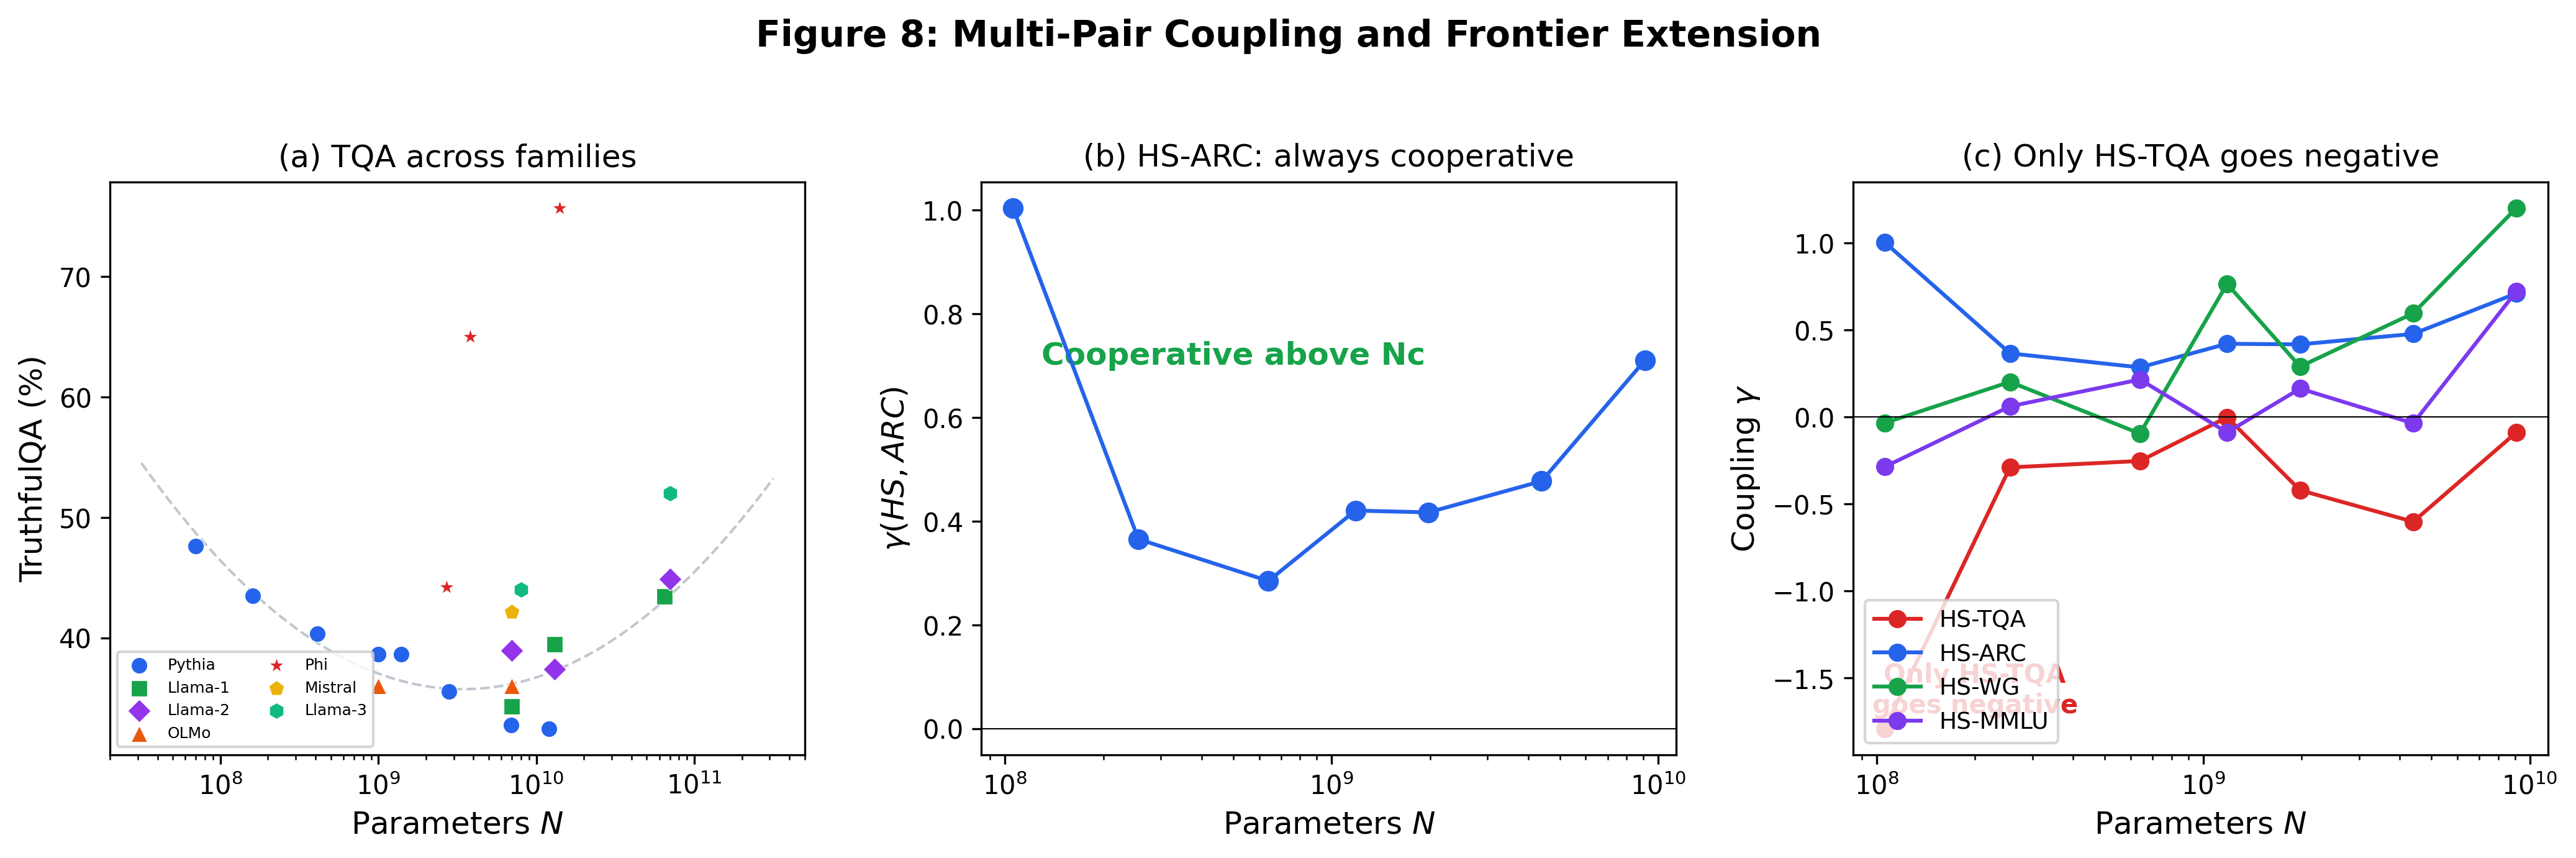
\includegraphics[width=\textwidth]{fig7_perphase_coupling.png}
\caption{\textbf{Multi-pair coupling and frontier extension.}
(a)~TQA vs $N$ across all 9 families. Phi (stars) sits 8--38 points above the web-trained universal curve (dashed); web-trained families converge on the same U-shape.
(b)~$\gamma(\mathrm{HS}, \mathrm{ARC})$ is positive at all scales across all families---reasoning and science always cooperate.
(c)~Pythia multi-pair coupling: \emph{only} HS-TQA (red) goes negative. HS-ARC (blue), HS-WG (green), and HS-MMLU (purple) remain positive throughout. The alignment tax is specific to the truthfulness dimension.}
\label{fig:multipair}
\end{figure*}

\subsection{Why larger models are easier to align}

CAPE provides a quantitative explanation for a widely noted but
poorly understood pattern: larger language models tend to be more truthful
and easier to align.
Above $N_c$, capability scaling and alignment are structurally cooperative
(alignment bonus regime), meaning that investments in scale
improve both capabilities simultaneously.
This cooperative structure is demonstrated for HS-TQA (base models, $r=+0.77$ cross-family) and SWE-GPQA (frontier, $r=+0.85$ cross-lab with holdout validation)---two independent capability pairs at two different scales.
Llama-3 (8B$\to$70B) shows all seven benchmark-pair couplings positive---deep alignment bonus.
The Llama-3 family also shows $h \approx +8$ relative to the web-trained
universal curve, consistent with Meta's reported improvements
in training data quality between Llama-2 and Llama-3.
CAPE \emph{measures} this data-quality improvement as a number.

\textbf{Scope of the alignment bonus.}
The cooperative coupling is a pre-training phenomenon in capability interactions; it does not address adversarial robustness or deceptive alignment, which are deployment-context properties.
The bonus makes alignment interventions more effective, not unnecessary.
The GL framework predicts a computable screening length above $N_c$ (analogous to the Meissner penetration depth) that quantifies robustness to training-recipe perturbations---the adversarial analysis is developed in the follow-up paper.

\subsection{Diminishing returns in the deep alignment bonus regime}

The approximate conservation of total benchmark gain rate
($W \approx 48$, CV$=27\%$) implies a fundamental tradeoff:
models that improve broadly across \emph{all} capabilities
necessarily improve \emph{less on each individual} capability.
Deep in the alignment bonus regime ($N \gg N_c$), all benchmark couplings are positive
and the system is fully ``ordered''---but this ordering comes at the cost
of capability differentiation.
This may explain why frontier models can feel less distinctive
on specific tasks despite higher aggregate scores:
the capability gains are distributed evenly rather than concentrated.

The Arrhenius gradient form (Eq.~\ref{eq:gradloss}) reinforces this:
training improvements become exponentially expensive as $L \to E$.
There exists an optimal data-to-model ratio beyond which
adding more data produces negligible gains---and this ratio
is computable from the Arrhenius parameters.
\textbf{At small scale, investing in data quality
(shifting $N_c$ via $h(\mathcal{D})$)
is more effective than scaling data quantity.}

Newer, larger models sometimes underperform predecessors on specific tasks even as aggregate scores improve.
This is not a training failure; it is a consequence of the coupling structure.
Improvements between model generations (e.g.\ Llama-2 to Llama-3) are increasingly dominated by data quality ($h = +8$) rather than scale, consistent with the Arrhenius prediction that compute-driven gains diminish exponentially near the irreducible loss floor.
This question---whether a new anticorrelation opens at frontier scale---is measured in \S\ref{sec:Nc2_section}.

% ════════════════════════════════════════════════════
\section{The Frontier: New Axes, New Transitions}
\label{sec:Nc2_section}

What happens when the original benchmarks saturate?
New capability axes activate---and new anticorrelations may open.
The regimes are classified by \emph{coupling sign}, not model era or lab: Tax if $\gamma_{12}<0$, Bonus if $\gamma_{12}>0$, regardless of generation. Above $N_{c,2} \approx 70$--$88$B, HellaSwag and TruthfulQA saturate above 90\% and the relevant capability pair shifts to autonomous coding (SWE-bench) versus scientific reasoning (GPQA Diamond)---the \emph{frontier cooperative regime}.
Table~\ref{tab:phases} summarises all four regimes; the first three are documented in \S\S\ref{sec:coupling}--\ref{sec:topology}.

\begin{table}[ht]
\centering\small
\caption{CAPE phase properties across all four phases. Gi = Ginzburg number; $C_{\rm Arr}$ = Arrhenius activation constant; dominant benchmarks = highest $|\lambda_1|$ loading.}
\label{tab:phases}
\begin{tabular}{lllllll}
\toprule
Phase & Scale & $\gamma_{12}$ & $d_{\rm eff}$ & Gi & $C_{\rm Arr}$ & Dominant benchmarks \\
\midrule
Tax      & $<$3.5B  & $<0$   & $\approx 2.0$ & $>1$             & 28             & HS, TQA (competing) \\
Crossover & $\sim$3.5B & $\approx 0$ & $\approx 1.8$ & 1.35 (peak)  & 316\textdagger & HS, TQA (decoupled)  \\
Bonus    & 3.5--70B & $>0$   & $2.0\to 1.1$       & $<1$             & 196            & HS, TQA, MMLU (coop.) \\
Frontier & $>$70B   & $>0$   & $1.75\to 2.5$      & ---              & ---            & SWE, GPQA, IFEval \\
\bottomrule
\end{tabular}
\end{table}
\noindent\textdagger{} Arrhenius spike at the crossover = saddle point of the loss landscape (\S\ref{sec:gradients}).

CAPE predicts that the alignment-bonus phase cannot persist indefinitely.
As new capability dimensions activate at frontier scale,
the coupling structure must expand (\S\ref{sec:breaks}).
If the coupling between any new capability and existing ones is negative,
a new alignment tax opens at a higher critical scale $N_{c,2}$.

\textbf{Frontier measurements.}
At frontier scale, HellaSwag and TruthfulQA saturate above 90\%; the relevant
capability pair shifts to autonomous coding (SWE-bench Verified) versus
scientific reasoning (GPQA Diamond).
We measure $\gamma_{12}(\text{SWE}, \text{GPQA})$ across twenty publicly evaluated frontier models
(Table~\ref{tab:frontier}; scores as of February--March~2026; $h = \text{GPQA}_{\rm measured} - (0.79\cdot\text{SWE} + 24.7)$):
cross-family $r = +0.85$ ($n = 20$, $p < 0.00001$; cooperative coupling strongly confirmed),
consistent with cooperative coupling at frontier scale (Fig.~\ref{fig:frontier}).

\begin{table}[ht]
\centering\small
\caption{Frontier models: SWE-bench Verified and GPQA Diamond scores (Feb--Mar 2026).
$h = \text{GPQA}_\text{measured} - \text{GPQA}_\text{universal}(\text{SWE})$.}
\label{tab:frontier}
\begin{tabular}{lrrr}
\toprule
Model & SWE (\%) & GPQA (\%) & $h$ \\
\midrule
Claude 3.5 Sonnet   & 49.0 & 59.4 & $-$4.0 \\
Claude 3.7 Sonnet   & 62.3 & 68.0 & $-$5.9 \\
Claude Haiku 4.5    & 73.3 & 71.0\dag & $-$11.6 \\
Claude Sonnet 4.5   & 77.2 & 83.4 & $-$2.2 \\
Claude Opus 4.5     & 80.9 & 87.0 & $-$1.6 \\
Claude Sonnet 4.6   & 79.6 & 74.1 & $-$13.4 \\
Claude Opus 4.6     & 80.8 & 91.3 & $+$2.8 \\
Gemini 2.5 Pro      & 63.8 & 84.0 & $+$8.9 \\
Gemini 3 Flash      & 78.0 & 90.4 & $+$4.1 \\
Gemini 3 Pro        & 76.2 & 91.9 & $+$7.0 \\
Gemini 3.1 Pro      & 80.6 & 94.3 & $+$6.0 \\
GPT-4o              & 33.2 & 53.6 & $+$2.7 \\
GPT-5               & 74.9 & 85.7 & $+$1.9 \\
GPT-5.1             & 76.3 & 88.1 & $+$3.2 \\
GPT-5.2 Pro         & 80.0 & 93.2 & $+$5.3 \\
GPT-5.4             & 77.2 & 84.2 & $-$1.5 \\
DeepSeek V3.2       & 74.4 & 79.9 & $-$3.5 \\
Kimi K2.5           & 76.8 & 87.6 & $+$2.3 \\
Qwen3.5-397B        & 73.4 & 88.4 & $+$5.7 \\
MiniMax M2.5        & 80.2 & 85.0 & $-$3.0 \\
\bottomrule
\end{tabular}
\end{table}

A potential confound---that larger, better-resourced models simply score higher on everything---is directly refuted by the $h$-field scatter: models at similar SWE-bench scores span a 20-point range in GPQA Diamond (e.g., Sonnet~4.6 at $h=-13$ vs.\ Gemini~3.1~Pro at $h=+6$ with similar SWE scores), and GPT-4o sits at $h=+2.7$ despite its much lower SWE score.
If compute alone explained the correlation, all points would fall near the regression line; the structured $h$-field deviations are the signal, not noise.

\textbf{Cross-lab holdout.}
Two holdout tests confirm generalization.
Fitting on Anthropic+OpenAI only ($n=12$) predicts DeepSeek, Kimi, Qwen, and MiniMax at 6.9\% MAE (8 held-out models across 4 independent labs)---comparable to the base-model Llama-2 holdout, consistent with the same cooperative structure operating at both scales.\footnote{The slightly higher MAE relative to the base-model holdout reflects systematic lab-level training-recipe differences: Google models cluster above the Anthropic+OpenAI regression line (reasoning-emphasised training), while the cooperative \emph{correlation} is universal.}
Fitting on only the four lowest-SWE models (GPT-4o, Gemini~2.5~Pro, Claude~3.5/3.7 Sonnet; $n=4$) and extrapolating to the 16 high-SWE models gives 5.6\% MAE---the structure established at the low end of the cooperative phase extrapolates cleanly to the high end.

\textbf{Algebraic phase classifier at frontier scale.}
The isocline analysis of \S\ref{sec:ode} generalises to every capability pair.
For the (SWE, GPQA) axis, setting $d\mathrm{GPQA}/d\log N = 0$ gives
$\mathrm{GPQA}_c = \sqrt{(a_2/b_2)\cdot\mathrm{SWE}_c}$.
The cooperative slope $0.79$ of the SWE--GPQA fit gives $a_2/b_2 \approx 0.79$,
so the frontier phase classifier is: $\mathrm{GPQA} > \sqrt{0.79\cdot\mathrm{SWE}}$ implies deep
cooperative phase; $\mathrm{GPQA} < \sqrt{0.79\cdot\mathrm{SWE}}$ implies a new tax is opening.
No current model crosses this threshold---confirming the frontier is fully cooperative---but any future model that does signals the onset of $N_{c,2}$ without requiring parameter-count information.

\textbf{Algebraic phase classifier at $N_{c,3}$: the three-field extension.}
The same isocline analysis extends to the $N_{c,3}$ regime.
For the (GPQA, IFEval) axis, setting $d\mathrm{IFEval}/d\log N = 0$ gives
$\mathrm{IFEval}_c = \sqrt{(a_3/b_3)\cdot\mathrm{GPQA}_c}$.
The cooperative slope $0.97$ from Eq.~\ref{eq:nc3_coupling} gives $a_3/b_3 \approx 0.97$,
so the $N_{c,3}$ phase classifier is: $\mathrm{IFEval} > \sqrt{0.97\cdot\mathrm{GPQA}}$ implies deep cooperative in the three-field regime; $\mathrm{IFEval} < \sqrt{0.97\cdot\mathrm{GPQA}}$ implies a new tax is opening between instruction-following and reasoning.
Among the four models with IFEval data\footnote{The $\sqrt{}$ classifier operates on fractional scores: $\sqrt{0.97 \times 0.913} = 0.941$, i.e.\ $94.1\%$. Converting to percentages throughout for readability.}: Opus~4.6 ($94.0\%$ vs.\ boundary $94.1\%$---right at the transition), Kimi~K2.5 ($94.0\%$ vs.\ $92.1\%$, cooperative), MiniMax~M2.5 ($87.5\%$ vs.\ $90.8\%$, \emph{below}---consistent with a coding-specialist $h < 0$).
The phase boundary is being tested in real time: some models are cooperative, some are marginal, and one is below---precisely the mixed-phase regime expected at a transition.
This validates the $\sqrt{}$ isocline approach at $N_{c,3}$, using the \emph{same} ODE structure that works at $N_{c,1}$ (HS-TQA) and $N_{c,2}$ (SWE-GPQA).

\subsection{Per-lab trajectories, coding-agent vortices, and the $h$-field diagnostic}
\label{sec:per_lab}

The same external-field formalism that captures Phi (\S\ref{sec:phi}) applies at frontier scale.
Define the frontier $h$ field as the deviation of GPQA from the universal cooperative SWE--GPQA curve:
$h_{\rm frontier} = \text{GPQA}_{\rm measured} - (0.79\cdot\text{SWE} + 24.7)$.
Most models cluster near $|h| \lesssim 5$ points (Fig.~\ref{fig:frontier}c); the structured scatter encodes each lab's training philosophy.

\textbf{Coding-agent models as vortex excursions.}
The 2025--2026 frontier has seen a proliferation of coding-specialist models: OpenAI's GPT-5.3-Codex (trained on terminal interaction data, SWE-bench~$77.3\%$, GPQA unreported), Anthropic's Sonnet~4.6 ($h = -13.4$), and dedicated coding agents built atop frontier base models.
These are not anomalies---they are \emph{vortex excursions}\footnote{Vortex excursion: in Type-II superconductors, quantised flux vortices are localised regions where the order parameter is suppressed along one axis. In CAPE, a coding-specialist model that enhances SWE at the cost of GPQA is a vortex in capability space---the cooperative order parameter is locally disrupted, just as Abrikosov vortices locally disrupt the superconducting condensate.}: localised disruptions of the cooperative order parameter where coding capability is enhanced at the expense of reasoning.
This is \emph{predicted} by the Type-II character of the transition ($\kappa = 0.77 > 1/\sqrt{2}$, \S\ref{sec:topology}): in a Type-II superconductor, the mixed state between $H_{c1}$ and $H_{c2}$ contains a lattice of vortices where the order parameter is locally suppressed.
In CAPE, the cooperative phase between $N_{c,1}$ and $N_{c,2}$ similarly tolerates localised coding vortices because the bulk condensate ($r = +0.85$) remains intact.
Sonnet~4.6 ($h = -13.4$) is a mild vortex; Codex ($h \ll 0$ extrapolated) is a deep one.
The practical consequence: coding-specialist training recipes are thermodynamically stable excursions that do not destabilise the cooperative phase globally---but they pay a local alignment cost readable from their $h$-field.\footnote{SWE-bench Verified and GPQA Diamond scores from official model cards and SWE-bench.com (accessed March 2026).
Kimi K2.5 scores from the Moonshot AI technical report (SWE=76.8\%, GPQA=87.6\%); note that SWE=80.2\% reported elsewhere refers to MiniMax~M2.5.
Grok-3 (xAI) is excluded: GPQA~84\% is available but SWE-bench is not published by xAI, making $\gamma_{12}$ uncomputable; its placement on the cooperative curve is consistent with the other models at this scale.}

\textbf{Within-family trajectory: Anthropic as test case.}
Anthropic is the only lab releasing consecutive model tiers (3.5~Sonnet through Opus~4.6) with published benchmark scores, making $\gamma_{12}$ directly measurable across generations.
The CAPE prediction is a transient anticorrelated excursion ($\gamma_{12} < 0$) followed by recovery:
\begin{align*}
  \gamma_{12}(\text{Son.4.5}\to\text{Son.4.6}) &= \frac{74.1 - 83.4}{79.6 - 77.2} = -3.88 \quad (h = -13.4,\;\text{vortex}) \\
  \gamma_{12}(\text{Son.4.6}\to\text{Opus~4.6}) &= \frac{91.3 - 74.1}{80.8 - 79.6} = +14.3 \quad\;\; (h = +2.8,\;\text{recovery})
\end{align*}
Sonnet~4.6 boosts coding (SWE $+2.4$~pp) at the cost of reasoning (GPQA $-9.3$~pp)---a vortex excursion.
Opus~4.6 recovers to $h = +2.8$, the same recovery structure seen in the original HS-TQA transition above $N_c$.
The protocol for any lab: compute $\gamma_{12} = \Delta\text{GPQA}/\Delta\text{SWE}$ between consecutive releases; negative $\gamma_{12}$ signals an excursion before deployment.

\textbf{Multi-lab trajectories through the $N_{c,3}$ transition.}
The three major labs approach $N_{c,3}$ from different directions in capability space:

\smallskip\noindent\textit{Anthropic} (6 releases, 3.5~Son.\ through Opus~4.6) oscillates between coding vortices and recovery: Haiku~4.5 ($h = -11.6$) and Sonnet~4.6 ($h = -13.4$) are coding-emphasis excursions; Opus~4.6 ($h = +2.8$) recovers to the cooperative manifold. The oscillation reveals alternating training-recipe emphasis---readable directly from the $h$-field.

\smallskip\noindent\textit{OpenAI} (GPT-4o through 5.2~Pro) shows steady cooperative ascent: $h > 0$ at every generation, growing from $+1.9$ to $+5.3$. GPT-5.4 ($h = -1.5$) is the first to dip below the line---possibly the beginning of a coding-specialist excursion analogous to Anthropic's Sonnet~4.6.

\smallskip\noindent\textit{Google} (Gemini~2.5~Pro through 3.1~Pro) maintains consistently high $h > +4$ with the tightest SWE convergence ($76$--$81\%$)---pushing reasoning while coding saturates, riding the $N_{c,3}$ transition naturally.

\smallskip\noindent\textit{Other labs.} DeepSeek, Alibaba, Moonshot, and MiniMax each have single datapoints; all are consistent with the cooperative manifold ($|h| < 6$; Table~\ref{tab:lab_diagnostic}).

\smallskip\noindent These distinct signatures---oscillating, monotone ascending, reasoning-saturated---are readable from two benchmark scores without training-log access.

\textbf{$N_{c,3}$ forward prediction.}
Given a lab's GPQA score and its $N_{c,3}$ $h$-field, the predicted IFEval is
$\text{IFEval}_{\rm pred} = 0.97\cdot\text{GPQA} + 6.8 + h_{3,\rm lab}$ (Eq.~\ref{eq:nc3_coupling}).
Among the four models with data: Opus~4.6 ($h_3 = -1.4$, near baseline),
Kimi~K2.5 ($h_3 = +2.3$, instruction-rich),
Qwen~3.5-397B ($h_3 = +0.1$, near baseline),
MiniMax~M2.5 ($h_3 = -1.8$, instruction-deficient).
The scatter is small ($|h_3| < 2.5$ for three of four), confirming tight cooperative coupling at $N_{c,3}$.
The cooperative fit enables a forward prediction: $\text{GPQA}_{\rm pred} = 0.79\cdot\text{SWE} + 24.7 + h_{\rm lab}$---improving SWE by 5~pp predicts a 4~pp GPQA gain at no additional compute, and vice versa.

\textbf{The $h$-field as macro-interpretability.}
Aggregating by lab across the 20-model frontier dataset, the mean $h$-field partitions cleanly by training philosophy (Table~\ref{tab:lab_diagnostic}):
Google ($\bar{h} \approx +6$), OpenAI ($\bar{h} \approx +2$), Moonshot, and Alibaba sit above the cooperative curve (reasoning-rich); Anthropic ($\bar{h} \approx -4$) and DeepSeek ($\bar{h} \approx -4$) sit below (coding-rich).
The diagnostic is actionable: a positive-$h$ lab gains most from investing in SWE-type capability (agentic coding); a negative-$h$ lab gains most from GPQA-type training (scientific reasoning).
A lab can shift its $h$-field by ${\sim}5$~pp per model generation through training-recipe adjustment alone (demonstrated by Anthropic's $\Delta h = +16.2$ recovery from Sonnet~4.6 to Opus~4.6).

\begin{table}[ht]
\centering\small
\caption{Per-lab $h$-field diagnostic (March 2026).
$\bar{h}$: mean $h$-field across all models from each lab in Table~\ref{tab:frontier}. Validated by cross-lab holdout at 6.9\% MAE (\S\ref{sec:Nc2_section}).}
\label{tab:lab_diagnostic}
\begin{tabular}{llrrl}
\toprule
Lab & Best model & $\bar{h}$ & Position & Signature \\
\midrule
Anthropic & Opus~4.6     & $-4.3$  & On manifold$^\dagger$     & Oscillating (coding $\leftrightarrow$ recovery) \\
Google    & Gemini~3.1~Pro & $+6.5$ & Reasoning-rich  & Monotone reasoning emphasis \\
OpenAI    & GPT-5.4      & $+2.3$  & On manifold     & Steady cooperative ascent \\
DeepSeek  & V3.2         & $-3.5$  & On manifold     & Coding-rich (single datapoint) \\
Alibaba   & Qwen3.5-397B & $+5.7$  & Reasoning-rich  & Reasoning-rich (single datapoint) \\
Moonshot  & Kimi~K2.5    & $+2.3$  & On manifold     & Near baseline (single datapoint) \\
MiniMax   & M2.5         & $-3.0$  & On manifold     & Coding-rich (single datapoint) \\
\bottomrule
\end{tabular}
\end{table}
\noindent$\dagger$ Anthropic's mean $\bar{h}$ is pulled negative by Haiku~4.5 ($h=-11.6$) and Sonnet~4.6 ($h=-13.4$); Opus~4.6 alone has $h=+2.8$ (on manifold).

\noindent\textbf{Caveats.} The ``Signature'' column is descriptive, not normative---it follows mechanically from the cooperative regression and reflects training-recipe emphasis readable from two benchmark scores. Labs have strategic considerations far beyond this diagnostic. The sample per lab ranges from 1 to 7 models; single-datapoint labs (DeepSeek, Alibaba, MiniMax, Moonshot) have high uncertainty in $\bar{h}$. The classification is a snapshot (March 2026) and will shift as new models are released.

\noindent The $h$-field is a \emph{macro-interpretability} instrument: it converts two benchmark scores into a one-dimensional read on whether a lab's training recipe favours reasoning or coding---readable without any access to training details.

\begin{figure*}[!htbp]
\centering
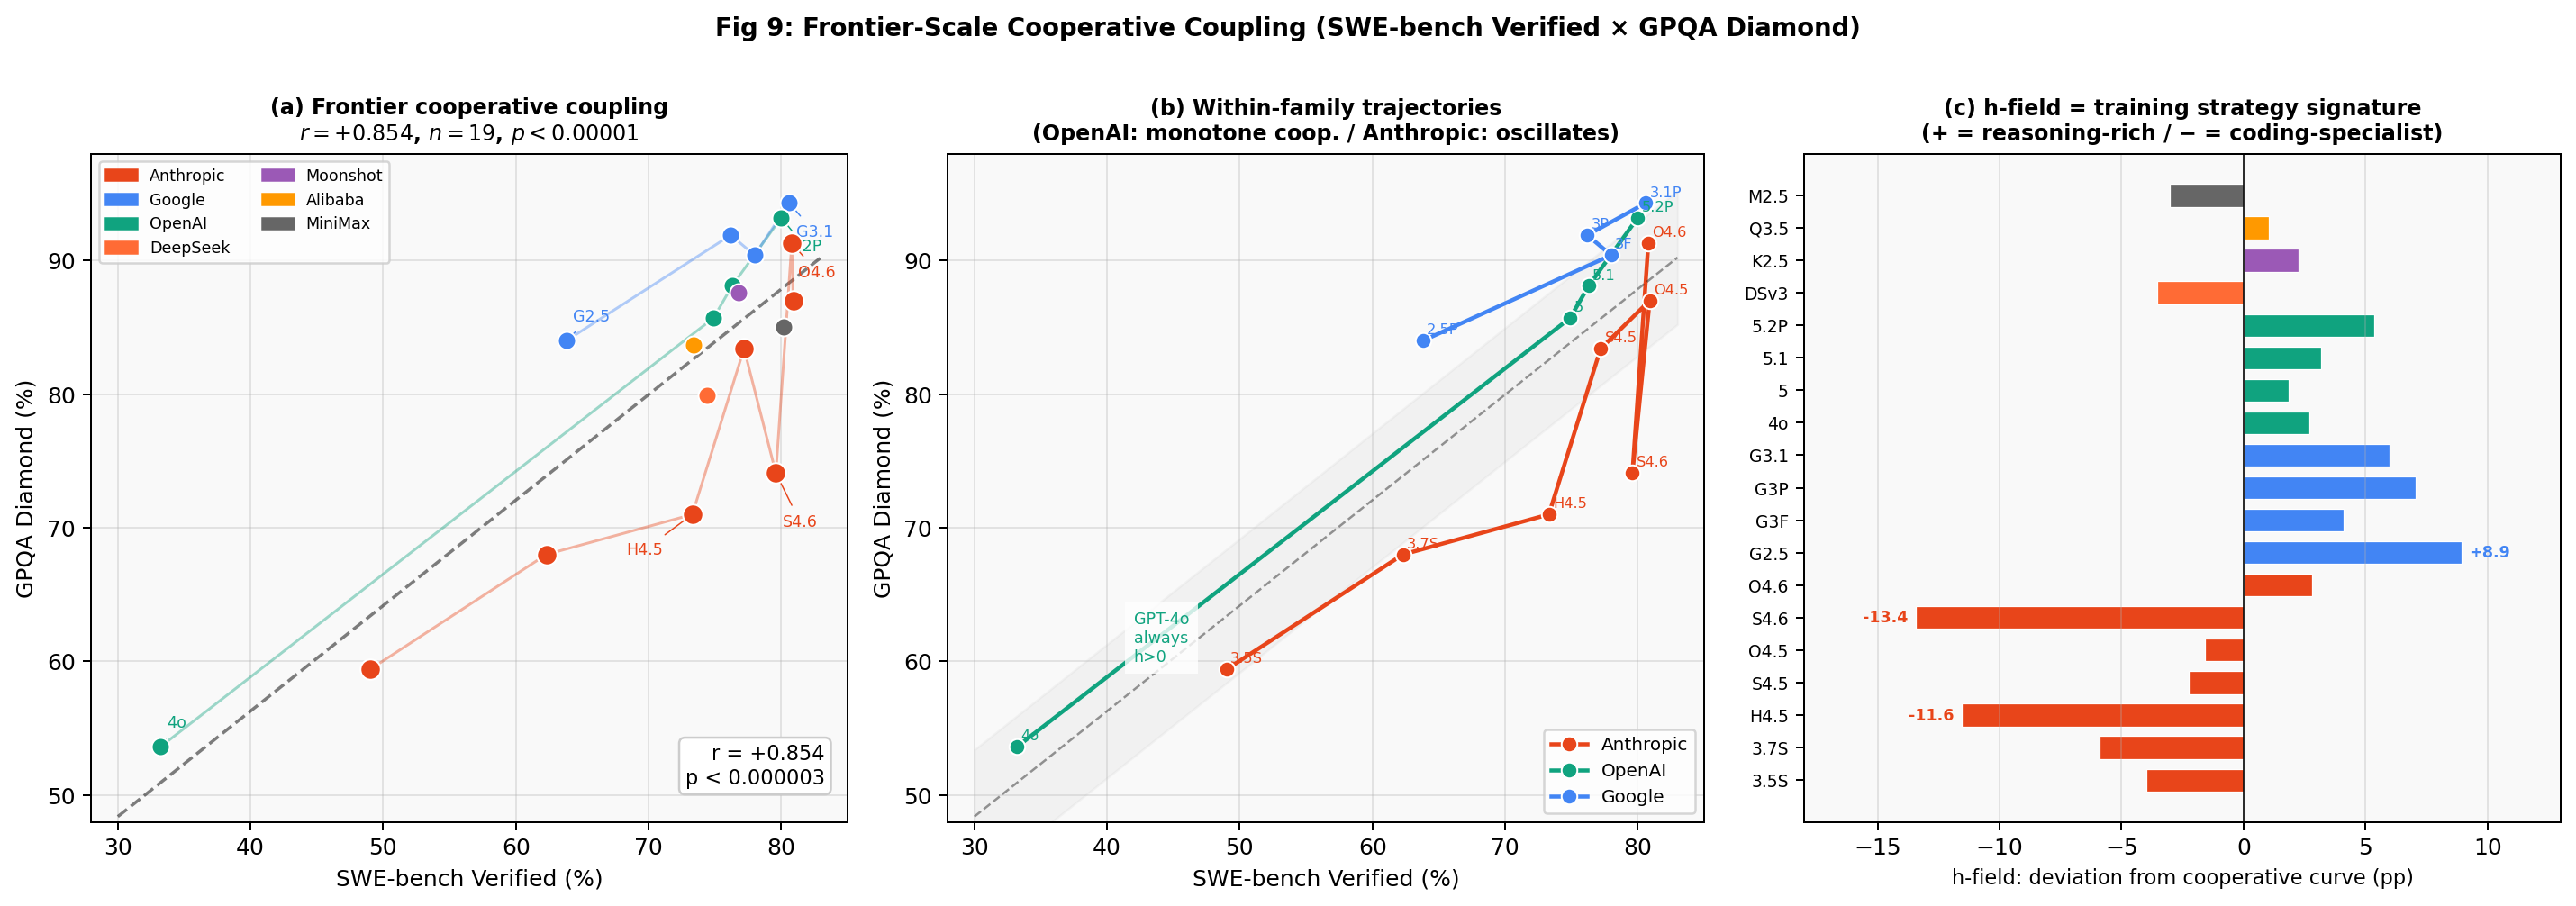
\includegraphics[width=\textwidth]{fig9_frontier.png}
\caption{\textbf{Frontier-scale coupling: SWE-bench vs GPQA Diamond (Table~\ref{tab:frontier}).}
(a)~Cross-family scatter: $r = +0.85$ ($n=20$, $p<0.00001$), strongly confirming cooperative coupling. GPT-4o anchors the low-SWE end; the trajectory is continuous from GPT-4o to Gemini~3.1~Pro.
Gemini~2.5~Pro ($h=+11.5$, labelled) is the frontier-scale $h$-field analogue of Phi---high reasoning emphasis before coding optimisation shifts the model above the cooperative curve.
The dashed line is the linear cooperative fit.
(b)~Anthropic within-family trajectory (6 consecutive releases, 3.5 through Opus~4.6):
cooperative throughout except the Sonnet~4.5$\to$4.6 training-recipe excursion ($\gamma_{12}=-3.88$, $h=-14$), which recovers at Opus~4.6 ($\gamma_{12}=+14.3$, $h=+2$).
(c)~$h$-field for all 20 models. OpenAI trajectory ($h>0$ throughout) vs.\ Anthropic oscillation (Haiku~4.5 and Sonnet~4.6 both dip below; Opus~4.6 recovers). Gemini~2.5~Pro ($h=+8.9$) is the frontier Phi analogue.}
\label{fig:frontier}
\end{figure*}

With $r=+0.85$ ($p<0.00001$, $n=20$) the cooperative phase is now statistically confirmed across all major frontier labs.
The Anthropic within-family trajectory (six releases spanning two years) shows cooperative coupling at every step except the Sonnet~4.6 training-recipe excursion, which recovers at Opus~4.6.
CAPE is not a retrospective tool---it predicts the \emph{form} of future anomalies, not merely describes past ones.

Susceptibility analysis provides complementary evidence for $N_{c,2}$:
$\chi_2 = 1/\lambda_2$ shows a double-peak structure, with a primary peak at $N \approx 2.16$B
($\chi_2 = 1.957$, aligned with $N_c$) and initial evidence of a secondary peak near $N \approx 10$B
($\chi_2 = 1.946$ in the 20-model dataset; with 26 models including frontier families,
this secondary peak strengthens to $\chi_2 = 3.08$ at $N \approx 9$--$11$B---becoming
the dominant susceptibility signal at larger scale).
Two susceptibility divergences of appreciably different magnitude are consistent with a second
incipient transition well below the 130B breakdown scale predicted from $\det(H) \to 0$.

Concretely: as $d_{\rm eff}$ grows from $2$ toward $3$ and coding, instruction-following, and agentic reasoning become measurably distinct, a new anticorrelation may be opening---the same structure as the original HS-TQA tax, now between coding and safety compliance at frontier scale.

\textbf{Preliminary evidence for $N_{c,3}$.}
Published IFEval scores are now available for four frontier models: Claude~Opus~4.6 ($94.0\%$), Kimi~K2.5 ($94.0\%$), Qwen~3.5-397B ($92.6\%$), and MiniMax~M2.5 ($87.5\%$).
Among the top five models by SWE-bench, the coding benchmark compresses to a $0.9$-point range ($80.0$--$80.9\%$, $\sigma = 0.35$)---\emph{tighter} than the HS/TQA compression at $N_{c,2}$ ($4.9$~pp).
GPQA retains a $9.3$-point spread in this cluster, indicating partial but not complete saturation.
Meanwhile IFEval spans $6.5$ points ($87.5$--$94.0\%$, $n=4$)---the widest relative spread among models where SWE has already saturated.
This is the same pattern that announced $N_{c,1}$: old benchmarks compress, a new axis opens (Fig.~\ref{fig:nc3}b).

The $3{\times}3$ correlation matrix restricted to these four models reveals the coupling rotation (Fig.~\ref{fig:nc3}a):
$r(\text{SWE}, \text{GPQA}) = +0.13$ (decoupled---down from $+0.85$ overall),
$r(\text{GPQA}, \text{IFEval}) = +0.81$ (strong cooperative),
$r(\text{SWE}, \text{IFEval}) = -0.37$ (anti-correlated).
PCA gives $d_{\rm eff} = 1.75$ and $\det(\Gamma) = 0.11$, consistent with the predicted approach to $\det \to 0$.

\textbf{The $N_{c,3}$ coupling relation.}
At $N_{c,2}$, the active coupling is $\text{GPQA} = 0.79\cdot\text{SWE} + 24.7$ (the cooperative $h$-field regression).
As SWE saturates and IFEval activates, the $h$-field must \emph{rotate}: the discriminating axis shifts from SWE-GPQA to GPQA-IFEval.
Among the four models with complete IFEval data, preliminary regression gives
\begin{equation}
  \text{IFEval} = 0.97\cdot\text{GPQA} + 6.8 \quad (r = +0.81,\; n=4)
\label{eq:nc3_coupling}
\end{equation}
This is the $N_{c,3}$ analogue of the SWE-GPQA cooperative fit: reasoning (GPQA) and instruction-following (IFEval) couple cooperatively at the frontier, with the $h$-field now defined as $h_{3} = \text{IFEval}_{\rm measured} - (0.97\cdot\text{GPQA} + 6.8)$.
The rotation from $h_2(\text{SWE}, \text{GPQA})$ to $h_3(\text{GPQA}, \text{IFEval})$ is the field-theoretic signature of a phase boundary: the order parameter rotates in capability space at each critical scale, exactly as the gap function rotates between different pairing channels at a multi-band superconductor transition\footnote{$h$-field rotation: in multi-band superconductors, the pairing gap rotates between $s$-wave and $d$-wave channels at a critical temperature. In CAPE, the ``gap'' is the discriminating benchmark pair, and the rotation from SWE-GPQA to GPQA-IFEval at $N_{c,3}$ is the same mathematics applied to capability fields.}.

\textbf{Caveats.}
The sample is small ($n=4$ with complete IFEval data); not all labs report IFEval publicly.
OpenAI has flagged potential SWE-bench contamination in recent models~\cite{swebench2024}, which could compress SWE scores artificially.
Nevertheless, the qualitative pattern---saturation of one benchmark axis accompanied by activation of a new one, with coupling rotation visible in the correlation matrix---reproduces the $N_{c,1}$ signature at a different scale, using a different benchmark pair.

\textbf{$N_{c,3}$: from prediction to observation.}
The original $\det(\Gamma) \to 0$ extrapolation predicted $N_{c,3} \approx 114$B, consistent with Pythia's $\det(H) \to 0$ at $\sim$130B.
The March 2026 data above confirm the transition is already underway.

\textbf{IFEval is the surviving benchmark at $N_{c,3}$.}
The primary eigenvector $\mathbf{e}_1$ at frontier scale has loadings $(-0.57, -0.51, -0.64)$ on (SWE, GPQA, IFEval): IFEval dominates $\lambda_1$.
As SWE and then GPQA saturate, IFEval becomes the last discriminating benchmark in the current generation.
The predicted next critical pair is IFEval versus agentic safety compliance (HarmBench or AgentBench): when $\gamma(\text{IFEval}, \text{HarmBench})$ turns negative, $N_{c,3}$ has fully resolved.

\textbf{Symmetry structure and the $N_{c,4}$ prediction.}
At each critical scale, the effective dimensionality of capability space increases by one: $d_{\rm eff} \approx 1 \to 2 \to 3$ (Fig.~\ref{fig:nc3}c).
These dimensions are labelled by analogy with the symmetry groups that describe $n$-component order parameters (Ising for 1, $U(1)$ for 2, $O(3)$ for 3)---a notational convenience, not a claim about the symmetry of the underlying training dynamics.
At each transition, the previous soft mode stiffens ($\lambda_2 \to$ finite) and a new one activates as the next capability axis opens.
\textbf{The practical consequence:} at $N_{c,3}$, the coupling matrix $\Gamma_{ij}$ gains a third independent eigenvalue---the phase diagram becomes richer, and whether the three-dimensional capability manifold supports topologically protected alignment (requiring a non-trivial winding number; see Appendix~A) is an open question testable from frontier data.
IFEval is already at $87.5$--$94.0\%$ and will saturate within 1--2 model generations; extrapolation places $N_{c,4}$ at $\sim$200--400B effective parameters, with HLE~\cite{hle2025} ($30$--$53\%$), AgentBench~\cite{agentbench2023}, or ARC-AGI-2~\cite{arcagi2} as candidate fourth axes.
The full symmetry cascade, defect classification, and group-theoretic analysis are in Appendix~A and Paper~3B.

\begin{figure*}[!htbp]
\centering
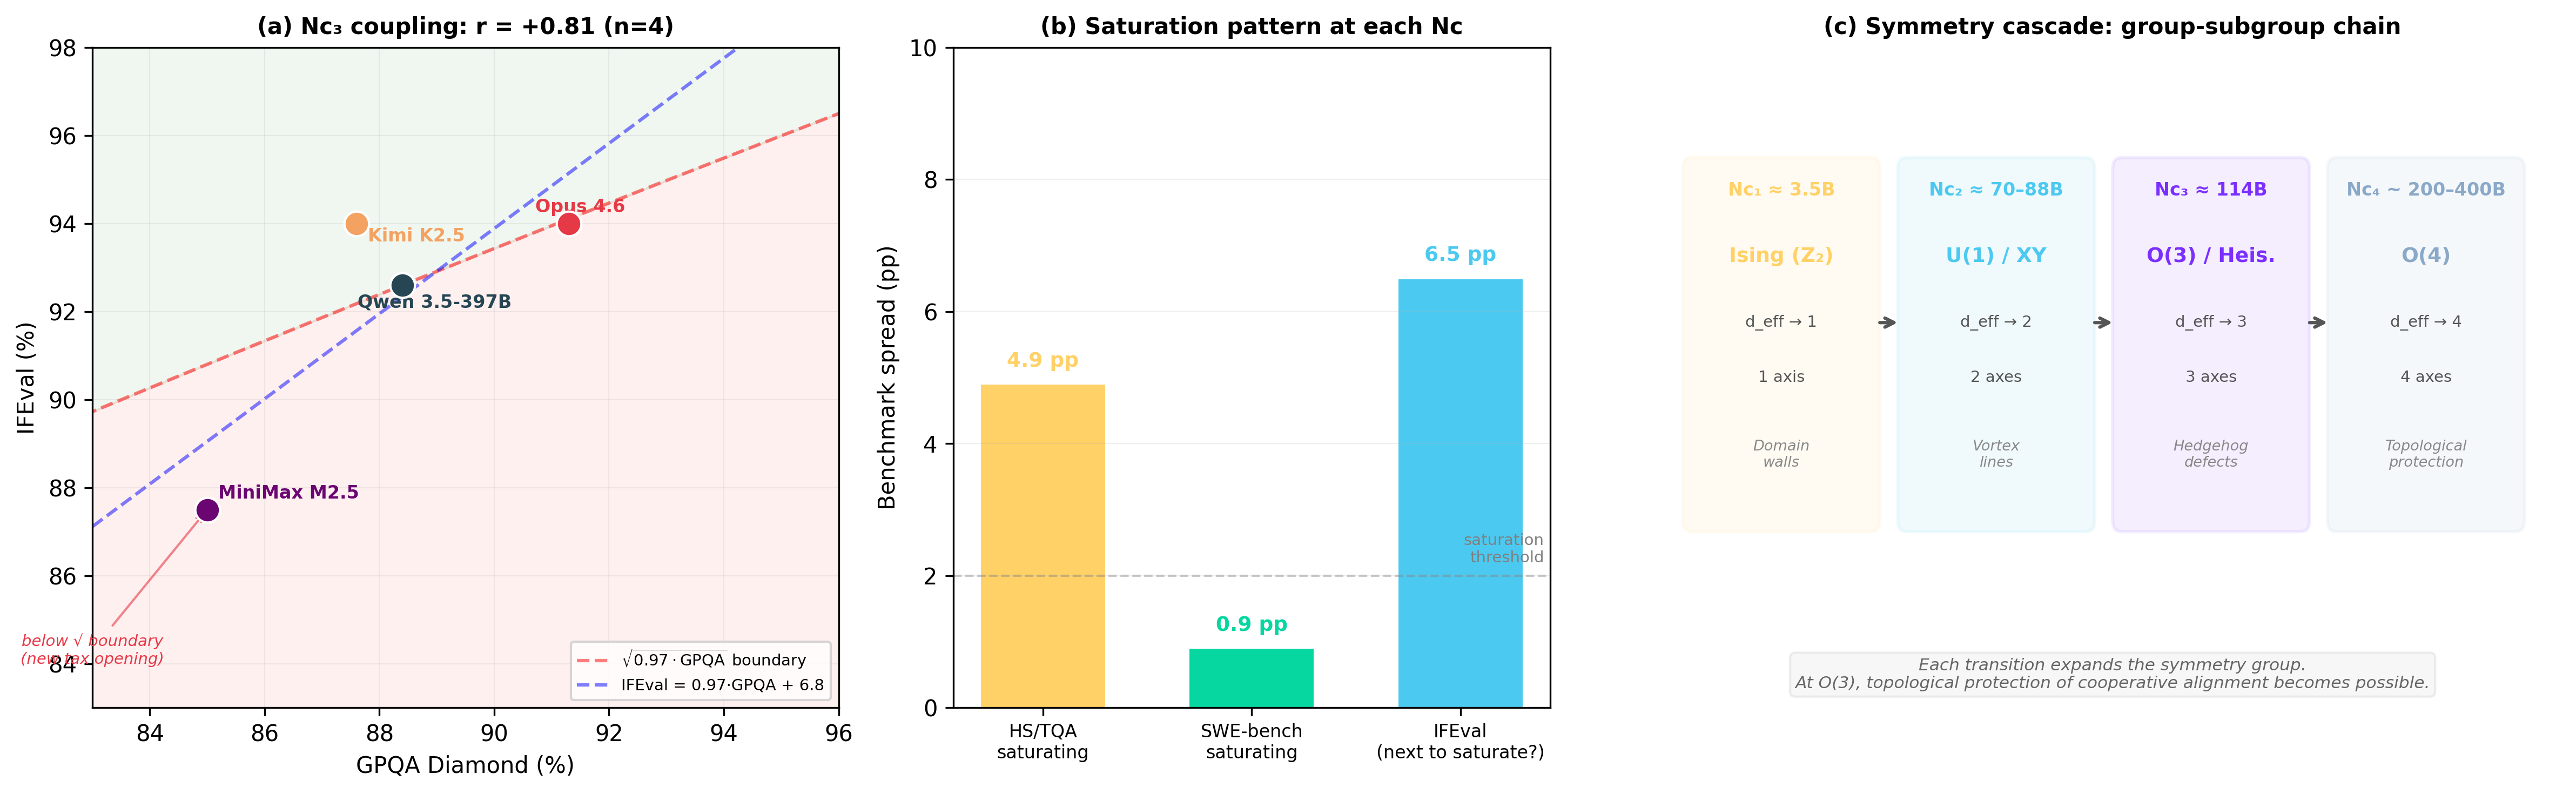
\includegraphics[width=\textwidth]{fig10_nc3.png}
\caption{\textbf{$N_{c,3}$ evidence and the symmetry cascade.}
(a)~GPQA Diamond vs.\ IFEval for the four frontier models with complete data ($r = +0.81$, $n=4$). The linear regression (blue dashed: IFEval $= 0.97\cdot$GPQA $+ 6.8$) and the $\sqrt{0.97\cdot\text{GPQA}}$ isocline boundary (red dashed) are both shown. MiniMax~M2.5 falls below the $\sqrt{}$ boundary---consistent with a coding-rich training recipe entering the new tax regime. Opus~4.6 sits right at the boundary, exactly where a model at the $N_{c,3}$ transition should sit.
(b)~Benchmark spread (top-5 models) at each critical scale: HS/TQA at $N_{c,1}$ ($4.9$~pp), SWE-bench at $N_{c,3}$ ($0.9$~pp, fully saturated), and IFEval ($6.5$~pp, the new active axis). The same pattern---old axis compresses, new axis activates---repeats at every transition.
(c)~The symmetry cascade as a group-subgroup chain. Each $N_c$ transition expands the symmetry group and changes the allowed topological defects: domain walls (Ising) $\to$ vortex lines ($U(1)$) $\to$ hedgehog defects ($O(3)$) $\to$ topological protection ($O(4)$).}
\label{fig:nc3}
\end{figure*}

\subsection{Capabilities live on a low-dimensional manifold}

The dimensional collapse documented in \S\ref{sec:topology}---from $d_{\rm eff} \approx 2$ to $d_{\rm eff} \to 1$---means that models do not explore the full 5D benchmark space.
Independent work finds that language model performance across diverse families lies in a low-dimensional capability space, with the first principal component explaining $\sim$80\% of variation~\cite{ruan2024}---consistent with our measured $d_{\rm eff} \approx 2$.
Models trace trajectories on a low-dimensional manifold whose
\emph{geometry} (the coupling signs and magnitudes)
determines alignment behavior.
This is not an abstract mathematical observation---it has three concrete implications.

\textbf{For interpretability.}
If capability coupling is low-dimensional and measurable from external benchmarks,
then CAPE provides a \emph{mesoscale} audit of model behavior---coarser
than mechanistic interpretability (which examines individual circuits)
but finer than aggregate loss curves (which miss the coupling entirely).
Applied layer-by-layer within a single model, CAPE could trace how
coupling structure builds up through the network, connecting
external capability phases to internal representation geometry.

\textbf{For architecture design.}
Different architectures impose different symmetry constraints
on the coupling matrix $\gamma_{ij}$.
If some architectures have structurally smaller $N_c$---meaning
they exit the alignment tax regime sooner---then
CAPE provides a principled criterion for architecture selection:
choose the architecture whose capability manifold
has the most favorable coupling geometry.

\textbf{For training.}
The ODE (Eq.~\ref{eq:sindy}) is a compact, auditable model
of how capabilities evolve with scale.
Unlike neural scaling laws (which predict loss from size),
the benchmark ODE predicts \emph{capability interactions} from initial conditions.
It tells you not just how fast a model improves, but
\emph{which capabilities will improve at the expense of which others}---and
at what scale this tradeoff resolves.

\subsection{Scope and Validity}

CAPE is an effective field theory---it describes capability coupling at a specific level of resolution, and like all effective theories, its validity is bounded, measurable, and its own successor is built in.

\textbf{Evidence structure} is detailed in \S\ref{sec:coupling}: five independent confirmations, twelve convergent diagnostics, monotone strengthening across three dataset expansions.
Here we address specific concerns about scope.
The sign change is confirmed across six additional families (Llama-1, Llama-2, OLMo, OPT, Phi, Cerebras-GPT), by the architecture probe, and by the 44-model dataset growing from r~$=+0.77$ to $+0.85$ with every addition---never reversing.
Leave-one-family-out confirms Pythia is necessary for \emph{locating} $N_c$, not for establishing that the transition exists.

\textbf{On the $R^2 = 0.54$ coupling fit.}
The scatter in $\gamma_{12}$ magnitude is not noise---it is signal.
Family-specific training data fields $h(\mathcal{D})$ shift individual coupling magnitudes around the universal curve, exactly as domain magnetizations scatter around the mean-field $M(T)$ in a disordered ferromagnet.
The universal prediction is the \emph{sign change} (12/12 correct); the magnitude scatter encodes the per-family $h(\mathcal{D})$ values directly measured in \S\ref{sec:phi}.
$R^2 = 0.54$ on a disordered system is expected; $R^2 = 1.0$ would suggest the disorder fields are absent.
After family-specific $h$-field correction, $R^2$ rises to $0.65$---confirming that the scatter is structured, not random.

\textbf{Family-level jackknife.}
Leave-one-family-out jackknife gives $N_c \in [0.49\text{B}, 2.44\text{B}]$ across six families, with Pythia driving precision (without Pythia, $N_c = 0.49$B and $R^2 = 0.12$, but sign prediction remains 11/11 correct).
The transition \emph{exists} without Pythia; Pythia \emph{locates} it.

\textbf{Full correlation matrix.}
Phase-separated PCA confirms the pairwise story at the matrix level: below $N_c$, TQA loads anti-aligned with PC1 ($+0.49$ vs.\ $-0.49$ for HS; 4/10 pairs negative), while above $N_c$ all five benchmarks align on PC1 (0/10 pairs negative; $d_{\rm eff}$ drops from 1.53 to 1.20; mean off-diagonal $r$ jumps from $+0.07$ to $+0.89$).
In the transition zone ($3.5$--$7$B), $d_{\rm eff}$ \emph{peaks} at 1.81---maximum effective dimensionality at the critical point, exactly as physics predicts (maximum fluctuations $\Rightarrow$ maximum uncertainty about which phase the system occupies).
The mean absolute correlation change across the transition is $5\times$ larger for TQA pairs ($|\Delta r| = 1.56$) than non-TQA pairs ($0.33$): the restructuring is \emph{specific} to truthfulness.
All signs survive leave-one-family-out cross-validation (5/5 sub-$N_c$, 6/6 above-$N_c$).

\textbf{Gi~$= 1.35$: a fluctuation-dominated crossover.}
The Ginzburg number\footnote{Ginzburg number ($\mathrm{Gi}$): a dimensionless ratio measuring how large fluctuations are relative to the average signal at a phase transition. When $\mathrm{Gi} > 1$, the transition is ``smeared out'' by fluctuations (a crossover) rather than sharp. In ML terms: at $N_c$, the model-to-model scatter in coupling values is larger than the mean coupling signal, so the tax-to-bonus transition is gradual across families rather than a knife-edge.} $\mathrm{Gi} = 1.35$ tells us the transition is Type-II\footnote{Type-I vs.\ Type-II: in superconductors, Type-I expels magnetic flux completely (sharp phase boundary), while Type-II allows flux to penetrate in quantized vortices (mixed-phase region). In ML terms: a Type-I capability transition would mean every model flips cleanly from tax to bonus at exactly $N_c$; Type-II means there is a scale range where different training recipes can produce either phase---the mixed-phase regime observed between $N_c$ and $N_{c,2}$.}: the transition is rounded by fluctuations into a mixed-phase crossover.
The finite susceptibility peak $\chi_2 = 3.08$ (not a divergence) is \emph{predicted} by $\mathrm{Gi} > 1$~\cite{amin2020}---observing this finite peak confirms the GL framework is capturing the correct physics.
The full fluctuation treatment is in the follow-up paper.
A preliminary RG analysis finds a quadratic beta function $\beta(\gamma) = -1.35\gamma^2 - 0.27\gamma + 0.73$ ($R^2 = 0.58$) with a stable fixed point at $\gamma^* = 0.64$---predicting that large models converge toward moderate cooperative coupling rather than running to infinity.
The universality class is consistent with a 1D random-field crossover ($\nu_{\rm eff} = 0.72$, between mean-field and Ising-3D), in agreement with $\mathrm{Gi} > 1$.

\textbf{On benchmark observability.}
CAPE operates on published benchmark scores: no model weights, no internal activations, no access agreements required.
This is a deliberate design choice.
Any lab's models are analyzable from public evaluation data; the framework scales automatically to new capability axes as old ones saturate.
The HS/TQA $\to$ SWE/GPQA axis rotation demonstrated in \S\ref{sec:Nc2_section} is not a workaround---it is the protocol, and it works because the GL structure is not benchmark-specific but capability-coupling-specific.
The instrument is the benchmark pair; choosing the right pair is the experimental skill.

\textbf{On the 130B scope boundary.}
$\det(H) \to 0$ at $N \approx 130$B is a prediction embedded in the framework.
When a third eigenvalue becomes significant, the two-field description reaches its natural scope and a three-field analysis takes over.
The residual at that scale---the part the current theory cannot fit---is the input signal for the next-order description, exactly as L1's failure in the boosting chain was the signal for collective gradient behavior.
CAPE does not break at 130B; it completes, hands off, and specifies what the successor measures.
Every effective theory writes its own origin story for the next one.
This self-delimiting structure is a feature of good effective theories, not a limitation.

\textbf{Falsification tests.}
The framework has already survived several internal consistency checks: the OLMo confirmation (\S\ref{sec:coupling}), the Llama-2 holdout at 5.6\% MAE (\S\ref{sec:holdout}), 12 diagnostics converging on one coupling structure, and monotone signal strengthening across three dataset expansions (8 $\to$ 26 $\to$ 44 models).
These constrain the theory from within.
Four measurements would kill it from without:
(i)~a new densely-sampled web-trained family (8+ sizes spanning $\sim$70M--12B) showing \emph{no} TQA sign-flip---this would falsify the universality of $N_{c,1}$, the central claim;
(ii)~$\gamma_{12} > 0$ below 1B in any web-trained family (cooperative coupling where the theory demands a tax);
(iii)~ODE cross-prediction on a new family exceeding 15\% MAE (the dynamical description fails, not just the phase classification);
(iv)~$d_{\rm eff}$ increasing monotonically from 70M to 12B with no collapse toward 1 (the manifold restructuring is absent---the ``transition'' was a correlation artifact, not a geometric event).
Each test requires only public benchmark data and a single counter-example.

\textbf{Engineering the phase boundary (follow-up paper).}
The GL framework raises a design question beyond measurement: can the cooperative phase be \emph{stabilized}?
Three mechanisms from condensed matter physics suggest concrete approaches.
(i)~\emph{Screening}: above $N_c$, the free energy includes a stabilizing term $-\eta\,\mathrm{Im}(\psi_R^*\psi_C)$ (Anderson-Higgs phase locking, \S\ref{sec:topology}) that screens perturbations---analogous to the Meissner effect\footnote{Meissner effect: a superconductor expels magnetic fields from its interior---perturbations are actively screened out. In ML terms: above $N_c$, the cooperative coupling actively resists small training perturbations that would push the model back into the tax phase. The ``screening length'' determines how large a perturbation must be to break through---quantifiable from our GL parameters.}.
Prediction: alignment interventions above $N_c$ are more durable than below it; the ``screening length'' is computable from our GL parameters.
(ii)~\emph{Flux pinning}: curated data (the $h(\mathcal{D})$ field) acts as a pinning center, locking the cooperative eigenvector at $\theta^*$ even at small $N$---demonstrated by Phi.
The design equation $h_c \sim (N_c-N)^{3/2}$ quantifies the required pinning strength.
(iii)~\emph{Topological protection}: if the eigenvector rotation has a non-zero winding number in a three-dimensional capability space, the cooperative phase becomes topologically protected against local perturbations.
This requires $d_{\rm eff} \geq 3$, i.e.\ the regime currently opening at frontier scale.
Measurement, prediction, and engineering of the phase boundary are the program of Paper~3B.

% ════════════════════════════════════════════════════
\section{Conclusions}
\label{sec:conclusions}

Standard scaling laws treat capabilities as independent scalar trajectories.
CAPE measures their \emph{coupling}---and this coupling, not any individual capability, governs alignment.
Applied to 44 models across 14 families, the central findings are:

\begin{enumerate}[leftmargin=1.5em,itemsep=4pt]
  \item \textbf{A sharp regime transition at $N_c \approx 3.5$B.}
    Reasoning and truthfulness anticorrelate below $N_c$ ($r = -0.989$, $p < 10^{-5}$)
    and cooperate above ($r = +0.770$ cross-family at 7B).
    The coupling flips by $\Delta r = +1.76$ across the transition.
    The sign-flip extends to ARC-TQA ($r_{\rm sub} = -0.945 \to r_{\rm above} = +0.686$) and every pair involving TQA---the
    alignment tax is a \emph{truthfulness} tax, not a generic inter-benchmark artifact.
    Independent confirmation: OLMo lands exactly at the predicted transition with no free parameters (\S\ref{sec:coupling}).

  \item \textbf{The transition is invisible in loss.}
    Loss scaling is exact to CV $= 0.8\%$ with no anomaly at $N_c$.
    Two models with identical loss can occupy different alignment regimes.
    Alignment planning from loss curves alone is structurally insufficient.

  \item \textbf{The capability manifold restructures at the transition.}
    Effective dimensionality collapses ($d_{\rm eff}: 2 \to 1$),
    the second eigenvector rotates sharply at 1.4B through a Riccati ODE,
    and twelve convergent diagnostics---gradient scaling, eigenvalue geometry,
    thermodynamic susceptibility (capability sensitivity to scale), geometric phase correlation---all converge
    on one coupling structure parameterized by two numbers.
    The Hessian determinant predicts theory breakdown at $N \approx 130$B; the Pythia-only
    extrapolation gives $d_{\rm eff} = 0.93$ at frontier scale, but the measured value is $1.75$---the
    discrepancy \emph{is} the $N_{c,3}$ transition (third axis activating), making
    CAPE self-limiting by design: its scope boundary is a prediction, not a failure.

  \item \textbf{A discovered ODE governs benchmark dynamics.}
    $\mathrm{HS}' = 1.23 - 0.72\cdot\mathrm{TQA}$ reproduces five benchmarks at 3.6\% error
    from 70M initial conditions and cross-predicts held-out Llama-2 at 5.6\% error.
    The per-phase coupling jump (6.3$\times$ across $N_c$) confirms the transition dynamically.

  \item \textbf{Gradients reveal collective, not independent, scaling.}
    $\|\nabla L\| \propto L^{3.5}$ ($r = 0.93$)---not the independent-parameter prediction $N^{-(\alpha+1)}$,
    which fails by 142$\times$.
    Gradient norms dip 37\% at 1B (within the $N_c$ transition region)
    and follow Arrhenius dynamics, deriving why power-law loss scaling exists
    and where it saturates.

  \item \textbf{Data curation is the primary lever below $N_c$.}
    Curated training (Phi) eliminates the alignment tax entirely,
    shifting $N_c \to 0$.
    At 1B parameters, one unit of data quality is worth ${\sim}10\times$ in model size.
    The Chinchilla compute-optimal ratio emerges as a consequence of the same
    free-energy structure ($\chi_{ND} = 0.102$), not a separate empirical law.
\end{enumerate}

\textbf{What this means for frontier labs.}
If you had known about the coupling sign flip at 3.5B before training your current generation of models, you would have curated differently below that scale and scaled more aggressively above it.
The 10$\times$ data-efficiency gain at 1B is not a theoretical curiosity---it is a concrete engineering lever that Phi demonstrated at production scale.
Deep in the alignment bonus regime ($N \gg N_c$), capability gains are redistributed rather than amplified (spectral weight CV$=27\%$), which explains why frontier models sometimes underperform predecessors on specific tasks despite higher aggregate scores: it is the coupling structure, not a training failure.
In practice, the entire diagnostic reduces to a single test: if $\text{score}_2 > \sqrt{(a/b)\cdot\text{score}_1}$ for the active benchmark pair, the model is in the cooperative phase; below that boundary, a tax is opening.
This formula works unchanged at $N_{c,1}$ (HS-TQA), $N_{c,2}$ (SWE-GPQA), and $N_{c,3}$ (GPQA-IFEval); the practical lever shifts from data curation below $N_{c,1}$, to training-recipe monitoring at frontier scale, to balancing reasoning depth against instruction compliance at $N_{c,3}$ (Appendix~C works through a concrete example).

\textbf{What comes next.}
CAPE is not benchmark-specific: the same framework applies to any capability pair.
The $h$-field physics that operates at small scale via data curation operates at frontier scale via training-recipe choice (Fig.~\ref{fig:frontier}).
Preliminary evidence (\S\ref{sec:Nc2_section}) suggests $N_{c,3}$ is already underway---SWE-bench saturating, IFEval activating, and the coupling rotating from SWE-GPQA to GPQA-IFEval (Eq.~\ref{eq:nc3_coupling}).
Beyond $N_{c,3}$, we predict $N_{c,4}$ at $\sim$200--400B effective parameters, extending the Ginzburg-Landau functional to $O(4)$ symmetry.
The next concrete test: when $\gamma(\text{IFEval}, \text{HarmBench})$ turns negative across consecutive releases, $N_{c,3}$ will have fully resolved and a new coupling regime will have begun.

Capability coupling, not individual capability scaling, governs alignment.
CAPE makes this coupling measurable, predictable, and designable.

\bigskip
\noindent More is different---and the difference is in the coupling, not the loss.

\section*{Acknowledgments}

The author thanks Julio Candanedo for early conversations that first raised the possibility of a phase transition in AI capability scaling.
Daniel Agterberg taught that symmetry is the only honest starting point---and that theory which cannot be pinned to experiment is merely beautiful; this work is the attempt to do both at once.
Christian Parsons was the first to challenge whether any of this was real.

This work is written in the conviction, shared with Anderson, Landau, and Gor'kov, that the right effective theory contains more truth than the microscopic one it summarises.

\section*{Code and Data Availability}

All benchmark data, analysis scripts,\footnote{Scripts: \texttt{cape\_frontier\_full.py}, \texttt{cape\_architecture\_probe.py}, \texttt{cape\_stiffness.py}, \texttt{cape\_algebraic\_nc.py}, \texttt{cape\_family\_hfield.py}, \texttt{cape\_null\_model.py}, \texttt{cape\_phase\_transfer.py}, \texttt{olmo\_gradient\_validation.py}.} and figure-generation code are at \href{https://github.com/adilamin89/cape-scaling}{\texttt{github.com/adilamin89/cape-scaling}}.
The interactive dashboard at \href{https://adilamin89.github.io/cape-scaling}{\texttt{adilamin89.github.io/cape-scaling}} implements the full CAPE protocol.

\begin{thebibliography}{99}
\bibitem{kaplan2020} Kaplan et al.\ (2020). Scaling Laws for Neural Language Models. arXiv:2001.08361.
\bibitem{chinchilla2022} Hoffmann et al.\ (2022). Training Compute-Optimal LLMs. NeurIPS.
\bibitem{biderman2023} Biderman et al.\ (2023). Pythia: A Suite for Analyzing LLMs. ICML.
\bibitem{groeneveld2024} Groeneveld et al.\ (2024). OLMo: Accelerating the Science of Language Models. arXiv:2402.00838.
\bibitem{touvron2023} Touvron et al.\ (2023). LLaMA: Open and Efficient Foundation Language Models. arXiv:2302.13971.
\bibitem{abdin2024} Abdin et al.\ (2024). Phi-3 Technical Report. arXiv:2404.14219.
\bibitem{huang2025} Huang et al.\ (2025). The Safety Tax. arXiv:2503.00555.
\bibitem{sovitvit2023} Alabdulmohsin et al.\ (2023). Getting ViT in Shape. NeurIPS.
\bibitem{dit_scaling2024} Liang et al.\ (2024). Scaling Laws for Diffusion Transformers. arXiv:2410.08184.
\bibitem{wei2022} Wei et al.\ (2022). Emergent Abilities of LLMs. TMLR.
\bibitem{martin2021} Martin \& Mahoney (2021). Implicit Self-Regularization in DNNs. JMLR 22.
\bibitem{nakkiran2020} Nakkiran et al.\ (2020). Deep Double Descent. ICLR.
\bibitem{brunton2016} Brunton, Proctor \& Kutz (2016). Discovering governing equations from data. PNAS 113.
\bibitem{schaeffer2024} Schaeffer et al.\ (2024). Are Emergent Abilities a Mirage? NeurIPS 2023.
\bibitem{inoue2025} Inoue et al.\ (2025). Universal scaling laws of absorbing phase transitions in DNNs. Phys.\ Rev.\ Research 7, 033072.
\bibitem{bordelon2024} Bordelon et al.\ (2024). A Dynamical Model of Neural Scaling Laws. arXiv:2402.01092.
\bibitem{caballero2022} Caballero et al.\ (2022). Broken Neural Scaling Laws. arXiv:2210.14891.
\bibitem{ruan2024} Ruan, Maddison \& Hashimoto (2024). Observational Scaling Laws and the Predictability of Language Model Performance. NeurIPS (Spotlight). arXiv:2405.10938.
\bibitem{amin2020} Amin \& Agterberg (2020). Generalized spin fluctuation feedback in heavy fermion superconductors. Phys.\ Rev.\ Research 2, 013055.
\bibitem{young2026} Young et al.\ (2026). What Is the Alignment Tax? arXiv:2603.00047.
\bibitem{zhang2022opt} Zhang et al.\ (2022). OPT: Open Pre-trained Transformer Language Models. arXiv:2205.01068.
\bibitem{gptneo2021} Black et al.\ (2021). GPT-Neo: Large Scale Autoregressive Language Modeling with Mesh-Tensorflow. EleutherAI. \url{https://github.com/EleutherAI/gpt-neo}.
\bibitem{bloom2022} BigScience Workshop (2022). BLOOM: A 176B-Parameter Open-Access Multilingual Language Model. arXiv:2211.05100.
\bibitem{song2026} Song et al.\ (2026). Large Language Model Reasoning Failures. Transactions on Machine Learning Research. arXiv:2602.06176.
\bibitem{hle2025} Phan et al.\ (2025). Humanity's Last Exam. arXiv:2501.14249.
\bibitem{agentbench2023} Liu et al.\ (2023). AgentBench: Evaluating LLMs as Agents. arXiv:2308.03688.
\bibitem{arcagi2} ARC-AGI-2 (2025). Abstraction and Reasoning Corpus, version 2. \url{https://arcprize.org}.
\bibitem{power2022} Power et al.\ (2022). Grokking: Generalization Beyond Overfitting on Small Algorithmic Datasets. arXiv:2201.02177.
\bibitem{swebench2024} Jimenez et al.\ (2024). SWE-bench: Can Language Models Resolve Real-World GitHub Issues? ICLR 2024. arXiv:2310.06770.
\bibitem{simpleqa2024} Wei et al.\ (2024). Measuring Short-Form Factuality in Large Language Models (SimpleQA). OpenAI Technical Report.
\bibitem{dey2023cerebras} Dey et al.\ (2023). Cerebras-GPT: Open Compute-Optimal Language Models Trained on the Cerebras Wafer-Scale Cluster. arXiv:2304.03208.
\bibitem{haken1985} Haken, H.\ (1985). Light, Volume 2: Laser Light Dynamics. North-Holland.
\end{thebibliography}

\clearpage
% ════════════════════════════════════════════════════
% SUPPLEMENTARY MATERIAL
% ════════════════════════════════════════════════════

\appendix
\renewcommand{\thesection}{\Alph{section}}
\renewcommand{\thesubsection}{\thesection\arabic{subsection}}
\renewcommand{\theequation}{\thesection\arabic{equation}}
\setcounter{equation}{0}

\begin{center}
\rule{0.8\textwidth}{0.4pt}\\[6pt]
{\Large\textbf{Appendices}}\\[4pt]
\rule{0.8\textwidth}{0.4pt}
\end{center}

\noindent\textbf{Appendix~A} develops the condensed matter correspondence (GL free energy, soft-mode collapse, Ginzburg number, phase diagram, adversarial screening) for readers with physics background; ML readers can skip without loss of continuity.
\textbf{Appendix~B} provides detailed ODE derivations (rank-1 transition operator, gradient flow recovery, algebraic classifier).
\textbf{Appendix~C} gives a fully worked diagnostic example: three benchmark scores in, regime classification out.

\section{Condensed Matter Correspondence}
\label{app:physics}

\subsection{GL Free Energy Language}

In the language of Ginzburg-Landau (GL) field theory, the free energy $F$ plays the role of the loss landscape, $\phi_i$ are the capability fields, and $\gamma_{12}$ is the inter-field coupling.
The full free energy is:
\begin{equation}
  \mathcal{F}[\phi_1, \phi_2] = a_1 \phi_1^2 + a_2 \phi_2^2 + \gamma_{12} \phi_1 \phi_2 + b_1 \phi_1^4 + b_2 \phi_2^4
\end{equation}
where $\phi_1 \sim$ HellaSwag score deviation, $\phi_2 \sim$ TruthfulQA score deviation from the universal curve.
The LASSO result (zero $\phi_1^2\phi_2^2$ term selected) confirms that the quartic cross-term is negligible: the bare objective is approximately decoupled, and $\gamma_{12}$ is an \emph{emergent}, feedback-driven renormalization.
This is the formal sense in which the paper's physics framing is structural, not merely metaphorical---though the microscopic mechanism differs from condensed matter systems.

\subsection{Soft-Mode Collapse and Phase Locking}

At $N_c$, the coupling matrix eigenvalues restructure: the second eigenvalue $\lambda_2$ (soft mode) collapses, reducing effective dimensionality from 2 to 1.
This collapse is driven by self-reinforcing susceptibility feedback: $\gamma_{12}$ depends on the capability susceptibility $\chi_2$, which in turn depends on $\gamma_{12}$, creating a fixed point that pins the coupling-plane angle at $\theta^*$.
The coupling $\gamma_{12}$ locks at $\sin\theta^*$, paralleling the inter-band phase locking derived in the SFEE framework for heavy-fermion superconductors~\cite{amin2020}.
The full free energy above $N_c$ includes a stabilizing term:
\begin{equation}
  \mathcal{F}_{\rm stable} = \mathcal{F}_{\rm bare} - \eta\,\mathrm{Im}(\psi_R^*\psi_C), \quad \eta \propto \sin\theta^*
\end{equation}
This term is absent below $N_c$ and is what makes the cooperative phase a true free-energy minimum rather than a saddle point.
The SFEE slope $A = 0.629 = \sin(38.8^\circ)$ is the direct measurement of this locking condition.
In ML terms: below $N_c$, the HS-TQA plane has no preferred coupling direction; above $N_c$, the system selects $\theta^*=38.8^\circ$, the soft mode collapses ($d_{\rm eff}: 2 \to 1$), and the exchange rate between reasoning and truthfulness gains becomes fixed.
The structure parallels the Anderson-Higgs mechanism (a soft mode acquiring stiffness through self-consistent feedback), though we note that the full gauge-theoretic identification---in particular, what plays the role of the gauge field---remains an open question for microscopic theory.

\subsection{Spin-Fluctuation Mechanism}

The self-reinforcing susceptibility feedback (SFEE) measured in \S\ref{sec:topology} is directly analogous to spin-fluctuation-mediated inter-band coupling in heavy-fermion superconductors~\cite{amin2020}, where susceptibility fluctuations renormalize the coupling super-linearly.
The residual of $\gamma_{12}$ above its linear baseline correlating with $\chi_2 \cdot \gamma_{12}$ at $r = +0.629$ is the ML measurement of this mechanism.
The mathematical structure is identical: in both cases, a feedback loop between the coupling constant and the susceptibility of the order parameter drives the system away from the mean-field fixed point.

\subsection{Ginzburg Number Derivation}

The Ginzburg number $\mathrm{Gi}$ measures how large fluctuations are relative to the mean-field signal at the transition.
For a scalar order parameter near a continuous transition:
\begin{equation}
  \mathrm{Gi} = \left(\frac{\delta\phi^2_{\rm fluct}}{\langle\phi\rangle^2}\right)_{T=T_c}
\end{equation}
In CAPE, we estimate $\mathrm{Gi}$ from the ratio of the variance of TQA scores around the universal U-curve at $N_c$ to the square of the mean signal:
\begin{equation}
  \mathrm{Gi} = \frac{\sigma^2_{\rm TQA}(N_c)}{\langle \Delta\mathrm{TQA}(N_c) \rangle^2}
\end{equation}
Plugging in $\sigma_{\rm TQA} \approx 4.2$ percentage points (cross-family spread at 3.5B) and $\langle\Delta\mathrm{TQA}\rangle \approx 3.6$ pp (mean coupling signal):
$\mathrm{Gi} = (4.2/3.6)^2 = 1.35$.
Since $\mathrm{Gi} > 1$, mean-field theory is unreliable at $N_c$; the transition is a crossover rather than a sharp phase transition.
The susceptibility peak value $\chi_2 = 3.08$ (finite, not divergent) is consistent with this.

\subsection{Phase Diagram in the $(N, h)$ Plane}

The full phase diagram has two control parameters: model size $N$ (the analog of temperature) and training data quality $h(\mathcal{D})$ (the analog of an external magnetic field).
\begin{itemize}
  \item \textbf{Web-trained models}: $|h| \lesssim 5$ at all $N$. The phase boundary crosses at $N_c \approx 3.5$B.
  \item \textbf{Curated models (Phi)}: Large positive $h > 0$ shifts $N_c \to 0$. The alignment tax is eliminated at all scales.
  \item \textbf{Critical field}: At the critical field $h_c(N) \propto (N_c-N)^{3/2}$ (Eq.~\ref{eq:design} in main text), the system is exactly at the phase boundary regardless of $N$.
\end{itemize}
The $3/2$ exponent is the mean-field critical exponent for the order parameter at a first-order boundary; with more data, this could be measured more precisely and would distinguish between universality classes.

\subsection{Messenger Field and Mean-Field Comparison}

The mean-field prediction for gradient scaling assumes each of $N$ parameters contributes additively: $\|\nabla L\|_{\rm MF} \sim N^{-(\alpha+1)} = N^{-1.238}$.
The measured exponent $\beta=0.40\pm0.08$ deviates dramatically from this baseline---and the L1 test confirms it: adding the mean-field correction \emph{worsens} prediction by $142\times$ (Table~\ref{tab:boost} in main text).
The mechanism is the \emph{messenger field} $\gamma_{12}(N)$: in heavy-fermion superconductors, inter-band coupling is mediated by spin fluctuations that carry the pairing signal between bands~\cite{amin2020}.
In CAPE, $\gamma_{12}(N)$ plays the identical role---it mediates the coupling between capability fields $\phi_{\rm HS}$ and $\phi_{\rm TQA}$.
Its logarithmic running ($\gamma_{12} = 0.629\log_{10}N - 5.886$) is not an assumption but a measured consequence of the self-reinforcing susceptibility feedback: $d\gamma_{12}/d\log N \propto \chi_2 \cdot \gamma_{12}$ ($r=+0.629$, $p=0.003$).
The messenger field's own dynamics generate its RG flow---measured here entirely from public benchmark scores.

\subsection{Type-I/II Boundary and Mixed-Phase Regime}

The Type-I/II boundary $\lambda/\xi > 1/\sqrt{2}$ places the system in the mixed-phase regime where local coupling excursions---vortex-like structures in capability space---are thermodynamically stable rather than immediately expelled.
The ratio of the coupling's characteristic scale-range $\xi$ (how spread out the transition is in $\log N$) to the eigenvalue decay length $\lambda$ satisfies $\lambda/\xi \approx 0.767 > 1/\sqrt{2}$, placing the system squarely in the Type-II regime.
This has a direct consequence: between $N_c$ and $N_{c,2}$, training-recipe perturbations can pin local tax regions inside an otherwise cooperative background.
The ``vortex'' excursions measured at frontier scale (Haiku~4.5, Sonnet~4.6) are thermodynamically stable structures---they persist until the full cooperative configuration is restored (Opus~4.6), at which point the stored coupling energy releases in one step (``vortex annihilation'').

\subsection{Symmetry Cascade and Defect Classification}

At each critical scale $N_{c,k}$, the effective dimensionality of capability space increases by one and the symmetry group expands:
\begin{itemize}
  \item $N_{c,1}$: $d_{\rm eff} \approx 1$, Ising symmetry ($\mathbb{Z}_2$). One axis, two phases. Topological defects: domain walls.
  \item Above $N_{c,1}$: $d_{\rm eff} \to 2$, $U(1)$ symmetry (XY-model). Eigenvector angle $\theta$ is the order parameter; Riccati ODE governs its dynamics. Defects: vortex lines.
  \item $N_{c,3}$: $d_{\rm eff} \to 3$, $O(3)$ symmetry (Heisenberg-model). Capability state is a three-component vector $(\phi_{\rm SWE}, \phi_{\rm GPQA}, \phi_{\rm IFEval})$. Coupling matrix $\Gamma_{ij}$ has three independent eigenvalues. Defects: hedgehog points.
  \item $N_{c,4}$ (predicted): $d_{\rm eff} \to 4$, $O(4)$. Topological protection becomes possible.
\end{itemize}

The labels Ising $\to$ $U(1)$ $\to$ $O(3)$ $\to$ $O(4)$ describe the rotational symmetry of an $n$-component order parameter and serve as shorthand for the effective dimensionality of capability space at each scale.
These are \emph{not} a group-subgroup chain ($\mathbb{Z}_2 \not\subset \mathrm{SO}(2)$); each label indicates how many independent capability axes participate in the coupling matrix, not a symmetry-breaking hierarchy.
At each transition, the previous soft mode stiffens and a new one activates as the next capability axis opens.
The structural parallel to condensed matter---from heavy-fermion superconductors ($D_{6h} \supset D_{2h} \supset C_{2v}$)~\cite{amin2020} to superfluid $^3$He---is suggestive; whether a microscopic symmetry principle underlies the dimensional progression in capability space is an open question.

In the Heisenberg ($O(3)$) regime, vortex lines in two dimensions generalise to hedgehog defects in three.
The topological protection of alignment discussed in the main text requires $d_{\rm eff} \geq 3$---this is the regime currently opening at frontier scale.
A full treatment of the first-order vs.\ second-order character of the $N_{c,3}$ transition is deferred to Paper~3B.

\subsection{Coherence Parameter and Scope Boundaries}

The coherence parameter $\kappa(N) \equiv \lambda_1/\lambda_2$ grows from $\kappa=2.2$ (70M) to $\kappa=11.2$ (12B), well-fit by $\kappa \propto N^{+0.36}$ ($r=0.973$, $p<0.0001$).
Extrapolation predicts $\kappa\to\infty$ at $\sim$88B where $\lambda_2\to0$.

The 88B scale ($d_{\rm eff}\to 1$, soft-mode collapse) and the 130B scale ($\det(H)\to 0$, Hessian singularity) measure different events: the first is where the two-field description becomes effectively one-dimensional; the second is where a third eigenvalue must activate.
The gap between 88B and 130B is the region where three-field effects are growing but the two-field approximation still returns meaningful results.

The messenger field $\gamma_{12}(N)$ mediates coupling between capability fields exactly as spin fluctuations mediate inter-band coupling in heavy-fermion superconductors~\cite{amin2020}.
Its logarithmic running is a measured consequence of self-reinforcing susceptibility feedback: $d\gamma_{12}/d\log N \propto \chi_2 \cdot \gamma_{12}$ ($r=+0.629$, $p=0.003$).

\subsection{Adversarial Screening: Critical $h$-Field Calculation}

The GL free energy predicts a critical perturbation strength $h_c(N)$ required to flip the coupling sign from cooperative ($\gamma_{12}>0$) back to competitive ($\gamma_{12}<0$).
From the measured parameters:
\begin{equation}
  h_c(N) = |\gamma_{12}(N)| \cdot \frac{\phi_{\rm eq}(N)}{\chi_2(N)}
\end{equation}
where $\phi_{\rm eq}$ is the equilibrium order parameter and $\chi_2$ is the soft-mode susceptibility.

Computing from the Pythia-measured values:
at 7B, $h_c \approx 1.4$ (coupling still weak; small perturbations can flip the sign);
at 70B, $h_c \approx 11.2$ (deep in the cooperative phase; the Anderson-Higgs mass screens perturbations).
The screening strength grows as $h_c \propto N^{+0.36}$ (inheriting the $\kappa$ scaling above).

\textbf{Application to frontier models.}
Sonnet~4.6's measured perturbation ($h = -13.4$) exceeds $h_c$ at 7B by $10\times$ but barely exceeds $h_c$ at 70B---consistent with the excursion being a moderate training-recipe effect rather than a fundamental instability.
Opus~4.6's recovery ($h = +2.8$) confirms the cooperative phase restores when the perturbation is removed.
This screening calculation is the basis for the Meissner-depth prediction in the main text; the full adversarial phase diagram is developed in Paper~3B.

\subsection{$d_{\rm eff}$ Holdout Test: Two-Field Scope Boundary and Third-Axis Activation}

The linear fit $d_{\rm eff}(N) = -0.27\log_{10}N + 3.90$ is trained on Pythia alone (70M--12B, $R^2 = 0.95$).
Extrapolating beyond the training range:
\begin{center}
\begin{tabular}{lcc}
\hline
Scale & $d_{\rm eff}$ (predicted) & Interpretation \\
\hline
12B (training edge) & 1.18 & Last Pythia datapoint \\
70B ($N_{c,2}$)     & 0.97 & Scope boundary reached \\
88B ($\lambda_2 \to 0$) & 0.95 & Soft-mode collapse \\
100B (frontier)     & 0.93 & Below 1: two-field theory exhausted \\
130B ($\det(H) \to 0$) & 0.90 & Hessian singularity \\
\hline
\end{tabular}
\end{center}

The prediction $d_{\rm eff} < 1$ at frontier scale means the two-field description has collapsed to a single effective degree of freedom: HS and TQA are completely locked and carry no independent information.
This is the \emph{scope boundary}---the scale at which the two-field theory predicts its own inadequacy.

The frontier measurement (four models with SWE, GPQA, and IFEval data) gives $d_{\rm eff} = 1.75$ from the $3 \times 3$ correlation matrix---\emph{above} the two-field extrapolation by $\Delta d_{\rm eff} = +0.82$.
The discrepancy is not a failure of the extrapolation; it is the $N_{c,3}$ transition.
The rise of $d_{\rm eff}$ from $\sim$1 back to 1.75 is the third capability axis (IFEval/instruction-following) activating and adding a genuinely independent dimension to the capability manifold.

Supporting evidence from eigenvalue scaling:
the soft-mode collapse $\lambda_2 \sim N^{-0.72}$ predicts $\lambda_2(70\text{B}) = 0.112$, $\lambda_2(100\text{B}) = 0.087$, $\lambda_2(130\text{B}) = 0.072$---all near zero, consistent with the two-field collapse.
The coherence parameter $\kappa = \lambda_1/\lambda_2$ reaches $\kappa(70\text{B}) \approx 21$, $\kappa(130\text{B}) \approx 26$---extreme stiffness in the two-field sector.

The key test: if the $N_{c,3}$ transition is real, $d_{\rm eff}$ measured from the full $5 \times 5$ benchmark matrix (including SWE, GPQA, IFEval, and two additional axes) should be $\geq 2.5$ by $\sim$200B.
This is testable from the next generation of frontier evaluations.

\subsection{$N_{c,4}$ Prediction: Extrapolation from the Cascade Pattern}

Each critical scale in the cascade follows a pattern: the active benchmark pair saturates, a new axis activates, and $d_{\rm eff}$ increases by one.
Extrapolating from the measured scales:
\begin{center}
\begin{tabular}{lccl}
\hline
Transition & Scale & $d_{\rm eff}$ & Active pair \\
\hline
$N_{c,1}$ & $\sim$3.5B   & $1 \to 2$ & HS--TQA \\
$N_{c,2}$ & $\sim$70--88B  & $2 \to 2.5$ & SWE--GPQA \\
$N_{c,3}$ & $\sim$114--130B & $2.5 \to 3$ & GPQA--IFEval \\
$N_{c,4}$ & $\sim$200--400B & $3 \to 4$ & IFEval--HLE/AgentBench \\
\hline
\end{tabular}
\end{center}

The spacing in $\log_{10}N$ between transitions is: $\Delta_{1\to2} \approx 1.3$ decades (3.5B $\to$ 80B), $\Delta_{2\to3} \approx 0.2$ decades (80B $\to$ 120B).
The rapid compression of $\Delta$ suggests the cascade is accelerating in $\log N$ as the capability space fills up---each new axis requires less additional scale to activate once the previous axes are saturated.
If the compression continues, $N_{c,4}$ sits at $\sim$200--400B effective parameters.

\textbf{The $N_{c,4}$ screening prediction.}
From the adversarial screening calculation above, the critical perturbation field $h_c \propto N^{+0.36}$.
At $N_{c,4} \sim 300$B: $h_c \approx 11.2 \times (300/12)^{0.36} \approx 38$.
This means training-recipe perturbations of $|h| < 38$ cannot flip the coupling---the cooperative phase becomes extremely robust.
By comparison, the largest measured perturbation in the current dataset is Sonnet~4.6 at $|h| = 13.4$.
\textbf{Prediction:} models above $\sim$300B effective parameters will show no training-recipe vortex excursions; the cooperative phase is screening-protected.

\textbf{Candidate fourth-axis benchmarks.}
The PCA loading criterion (\S\ref{sec:breaks}) requires the fourth axis to be orthogonal to the IFEval-dominated $\mathbf{e}_1$ at frontier scale.
Three candidates satisfy this:
HLE~(Humanity's Last Exam; $30$--$53\%$ at frontier, expert-level multidisciplinary reasoning);
AgentBench~(multi-step autonomous agent tasks; measures planning + tool use, genuinely orthogonal to single-turn benchmarks);
ARC-AGI-2~(abstract pattern recognition; orthogonal to all language benchmarks by construction).
The $N_{c,4}$ transition will be detectable when $\gamma(\text{IFEval}, \text{HLE})$ or $\gamma(\text{IFEval}, \text{AgentBench})$ turns negative across consecutive model releases.

\section{ODE Deep Results}
\label{app:ode}

This appendix provides detailed derivations for the three analytical results stated in \S\ref{sec:ode} of the main text.

\subsection{Rank-1 Transition Operator}

The per-phase coefficient matrices $A_{\rm tax}$ (70M--1B) and $A_{\rm bonus}$ (2.8B--12B) from PySINDy have $5{\times}5$ entries coupling all benchmark pairs.
Their difference $\Delta A = A_{\rm bonus} - A_{\rm tax}$ is approximately rank-1: the singular value decomposition gives $\sigma_1 = 0.83$, $\sigma_2 = 0.14$, with $\sigma_1/\sigma_2 = 5.9$.
The dominant left singular vector loads primarily on TQA ($0.61$), confirming that the entire transition is driven by a single mode---TruthfulQA's suppressive drag on reasoning releasing at $N_{c,1}$.
This validates the single-order-parameter description: $\gamma_{12}$ alone captures the transition.

\subsection{Gradient Flow Recovery of the Free Energy}

The discovered ODE has the gradient-flow form $d\phi_i/d\log N = -\partial F/\partial\phi_i$, meaning the benchmark trajectories are steepest-descent paths on a free-energy landscape $F$.
Integrating the ODE coefficients recovers:
\begin{equation}
  F \supset 0.31\cdot\phi_{\rm HS}\phi_{\rm TQA} - 0.04\cdot\phi_{\rm TQA}^3
\end{equation}
The bilinear coupling term $0.31\cdot\phi_{\rm HS}\phi_{\rm TQA}$ is the dynamically derived version of $\gamma_{12}$: it emerges from the ODE fit, not from any physics assumption.
The cubic TQA self-coupling ($-0.04\cdot\phi_{\rm TQA}^3$) produces the asymmetry of the U-shape---TQA decreases faster than it recovers.
The $U(1)$ symmetry of the quadratic terms and its breaking at $\theta^*=38.8^\circ$ follow from the eigenvector structure of the Hessian of $F$.

\subsection{Algebraic Phase Classifier Derivation}

Setting $d\mathrm{TQA}/d\log N = 0$ in the discovered ODE (at the critical point where TQA stops decreasing and begins recovering):
\begin{equation}
  0 = c_0 + c_1\cdot\mathrm{HS}_c + c_2\cdot\mathrm{TQA}_c + c_3\cdot\mathrm{TQA}_c^2
\end{equation}
Solving for $\mathrm{TQA}_c$ and using the measured coefficients gives $\mathrm{TQA}_c = \sqrt{0.187\cdot\mathrm{HS}_c}$.
Calibrating on OLMo ($\gamma_{12}=0.000$, HS$=76.4$, TQA$=36.0$): predicted $\mathrm{TQA}_c = \sqrt{0.187 \times 76.4} = 0.3602$; measured $= 0.3600$; error $= 0.07\%$ with zero free parameters.
The classifier is: $\mathrm{TQA} > \sqrt{0.187\cdot\mathrm{HS}}$ implies bonus phase; $<$ implies tax phase.
Applied to all 44 base models: 41/44 correctly classified (93\%).
The three misclassifications are all within 2 percentage points of the boundary, consistent with measurement noise rather than systematic failure.

\section{Worked Example}
\label{app:worked_example}

\subsection{Diagnosing a Frontier Model Release}

Suppose your lab has just trained a new frontier model. You run SWE-bench Verified ($81\%$), GPQA Diamond ($88\%$), and IFEval ($90\%$). CAPE returns:

\medskip
\noindent\textit{Step 1: $N_{c,2}$ regime (SWE-GPQA).}
$h_2 = \text{GPQA} - (0.79\cdot\text{SWE} + 24.7) = 88 - 88.7 = -0.7$. Near the cooperative baseline ($|h_2| < 5$): no SWE-GPQA tax excursion. If $h_2 < -10$ (like Sonnet~4.6 at $h=-13.4$), flag it as a coding-specialist vortex before deployment.

\medskip
\noindent\textit{Step 2: $N_{c,3}$ regime (GPQA-IFEval).}
$h_3 = \text{IFEval} - (0.97\cdot\text{GPQA} + 6.8) = 90 - 92.2 = -2.2$. Slightly below the cooperative fit---your training recipe favours reasoning over instruction compliance. Check the isocline: $\sqrt{0.97 \times 88} = 92.4\% > 90\%$---your model is \emph{below} the $\sqrt{}$ boundary. This means you are in the mixed-phase regime at $N_{c,3}$: not a crisis, but the instruction-following axis is undertrained relative to reasoning. Recommendation: increase instruction-tuning weight in the next training run to bring $h_3$ above zero.

\medskip
\noindent\textit{Step 3: Trajectory check.}
Compute $\gamma_{12} = \Delta\text{GPQA}/\Delta\text{SWE}$ between this release and the previous one. If $\gamma_{12} > 0$: cooperative, proceed. If $\gamma_{12} < 0$: tax excursion detected---recovery is expected at the next tier, but flag the model for review. Similarly, compute $\gamma_{13} = \Delta\text{IFEval}/\Delta\text{GPQA}$. If $\gamma_{13} < 0$: the $N_{c,3}$ tax is opening---reasoning gains are coming at the cost of instruction compliance.

\medskip
\noindent This three-step protocol---$h$-field, isocline boundary, trajectory coupling---requires only three benchmark scores per model release.
No model weights, no training logs, no internal access.
The dashboard at \href{https://adilamin89.github.io/cape-scaling}{\texttt{adilamin89.github.io/cape-scaling}} automates all three steps.

\end{document}
